%! TEX root = /home/user/Documents/KTH/notes/SF1626/main.tex
\documentclass{report}

%%%%%%%%%%%%%%%%%%%%%%%%%%%%%%%%%
% PACKAGE IMPORTS
%%%%%%%%%%%%%%%%%%%%%%%%%%%%%%%%%


\usepackage[tmargin=2cm,rmargin=1in,lmargin=1in,margin=0.85in,bmargin=2cm,footskip=.2in]{geometry}
\usepackage{amsmath,amsfonts,amsthm,amssymb,mathtools}
\usepackage[varbb]{newpxmath}
\usepackage{xfrac}
\usepackage[makeroom]{cancel}
\usepackage{mathtools}
\usepackage{bookmark}
\usepackage{enumitem}
\usepackage{hyperref,theoremref}
\hypersetup{
	pdftitle={Assignment},
	colorlinks=true, linkcolor=doc!90,
	bookmarksnumbered=true,
	bookmarksopen=true
}
\usepackage[most,many,breakable]{tcolorbox}
\usepackage{xcolor}
\usepackage{varwidth}
\usepackage{varwidth}
\usepackage{etoolbox}
%\usepackage{authblk}
\usepackage{nameref}
\usepackage{multicol,array}
\usepackage{tikz-cd}
\usepackage[ruled,vlined,linesnumbered]{algorithm2e}
\usepackage{comment} % enables the use of multi-line comments (\ifx \fi) 
\usepackage{import}
\usepackage{xifthen}
\usepackage{pdfpages}
\usepackage{transparent}

\newcommand\mycommfont[1]{\footnotesize\ttfamily\textcolor{blue}{#1}}
\SetCommentSty{mycommfont}
\newcommand{\incfig}[1]{%
    \def\svgwidth{\columnwidth}
    \import{./figures/}{#1.pdf_tex}
}

\usepackage{tikzsymbols}
\renewcommand\qedsymbol{$\Laughey$}


%\usepackage{import}
%\usepackage{xifthen}
%\usepackage{pdfpages}
%\usepackage{transparent}


%%%%%%%%%%%%%%%%%%%%%%%%%%%%%%
% SELF MADE COLORS
%%%%%%%%%%%%%%%%%%%%%%%%%%%%%%



\definecolor{myg}{RGB}{56, 140, 70}
\definecolor{myb}{RGB}{45, 111, 177}
\definecolor{myr}{RGB}{199, 68, 64}
\definecolor{mytheorembg}{HTML}{F2F2F9}
\definecolor{mytheoremfr}{HTML}{00007B}
\definecolor{mylenmabg}{HTML}{FFFAF8}
\definecolor{mylenmafr}{HTML}{983b0f}
\definecolor{mypropbg}{HTML}{f2fbfc}
\definecolor{mypropfr}{HTML}{191971}
\definecolor{myexamplebg}{HTML}{F2FBF8}
\definecolor{myexamplefr}{HTML}{88D6D1}
\definecolor{myexampleti}{HTML}{2A7F7F}
\definecolor{mydefinitbg}{HTML}{E5E5FF}
\definecolor{mydefinitfr}{HTML}{3F3FA3}
\definecolor{notesgreen}{RGB}{0,162,0}
\definecolor{myp}{RGB}{197, 92, 212}
\definecolor{mygr}{HTML}{2C3338}
\definecolor{myred}{RGB}{127,0,0}
\definecolor{myyellow}{RGB}{169,121,69}
\definecolor{myexercisebg}{HTML}{F2FBF8}
\definecolor{myexercisefg}{HTML}{88D6D1}


%%%%%%%%%%%%%%%%%%%%%%%%%%%%
% TCOLORBOX SETUPS
%%%%%%%%%%%%%%%%%%%%%%%%%%%%

\setlength{\parindent}{1cm}
%================================
% THEOREM BOX
%================================

\tcbuselibrary{theorems,skins,hooks}
\newtcbtheorem[number within=section]{Theorem}{Sats}
{%
	enhanced,
	breakable,
	colback = mytheorembg,
	frame hidden,
	boxrule = 0sp,
	borderline west = {2pt}{0pt}{mytheoremfr},
	sharp corners,
	detach title,
	before upper = \tcbtitle\par\smallskip,
	coltitle = mytheoremfr,
	fonttitle = \bfseries\sffamily,
	description font = \mdseries,
	separator sign none,
	segmentation style={solid, mytheoremfr},
}
{th}

\tcbuselibrary{theorems,skins,hooks}
\newtcbtheorem[number within=chapter]{theorem}{Sats}
{%
	enhanced,
	breakable,
	colback = mytheorembg,
	frame hidden,
	boxrule = 0sp,
	borderline west = {2pt}{0pt}{mytheoremfr},
	sharp corners,
	detach title,
	before upper = \tcbtitle\par\smallskip,
	coltitle = mytheoremfr,
	fonttitle = \bfseries\sffamily,
	description font = \mdseries,
	separator sign none,
	segmentation style={solid, mytheoremfr},
}
{th}


\tcbuselibrary{theorems,skins,hooks}
\newtcolorbox{Theoremcon}
{%
	enhanced
	,breakable
	,colback = mytheorembg
	,frame hidden
	,boxrule = 0sp
	,borderline west = {2pt}{0pt}{mytheoremfr}
	,sharp corners
	,description font = \mdseries
	,separator sign none
}

%================================
% Corollery
%================================
\tcbuselibrary{theorems,skins,hooks}
\newtcbtheorem[number within=section]{Corollary}{Corollary}
{%
	enhanced
	,breakable
	,colback = myp!10
	,frame hidden
	,boxrule = 0sp
	,borderline west = {2pt}{0pt}{myp!85!black}
	,sharp corners
	,detach title
	,before upper = \tcbtitle\par\smallskip
	,coltitle = myp!85!black
	,fonttitle = \bfseries\sffamily
	,description font = \mdseries
	,separator sign none
	,segmentation style={solid, myp!85!black}
}
{th}
\tcbuselibrary{theorems,skins,hooks}
\newtcbtheorem[number within=chapter]{corollary}{Corollary}
{%
	enhanced
	,breakable
	,colback = myp!10
	,frame hidden
	,boxrule = 0sp
	,borderline west = {2pt}{0pt}{myp!85!black}
	,sharp corners
	,detach title
	,before upper = \tcbtitle\par\smallskip
	,coltitle = myp!85!black
	,fonttitle = \bfseries\sffamily
	,description font = \mdseries
	,separator sign none
	,segmentation style={solid, myp!85!black}
}
{th}


%================================
% LENMA
%================================

\tcbuselibrary{theorems,skins,hooks}
\newtcbtheorem[number within=section]{Lenma}{Lenma}
{%
	enhanced,
	breakable,
	colback = mylenmabg,
	frame hidden,
	boxrule = 0sp,
	borderline west = {2pt}{0pt}{mylenmafr},
	sharp corners,
	detach title,
	before upper = \tcbtitle\par\smallskip,
	coltitle = mylenmafr,
	fonttitle = \bfseries\sffamily,
	description font = \mdseries,
	separator sign none,
	segmentation style={solid, mylenmafr},
}
{th}

\tcbuselibrary{theorems,skins,hooks}
\newtcbtheorem[number within=chapter]{lenma}{Lenma}
{%
	enhanced,
	breakable,
	colback = mylenmabg,
	frame hidden,
	boxrule = 0sp,
	borderline west = {2pt}{0pt}{mylenmafr},
	sharp corners,
	detach title,
	before upper = \tcbtitle\par\smallskip,
	coltitle = mylenmafr,
	fonttitle = \bfseries\sffamily,
	description font = \mdseries,
	separator sign none,
	segmentation style={solid, mylenmafr},
}
{th}


%================================
% PROPOSITION
%================================

\tcbuselibrary{theorems,skins,hooks}
\newtcbtheorem[number within=section]{Prop}{Proposition}
{%
	enhanced,
	breakable,
	colback = mypropbg,
	frame hidden,
	boxrule = 0sp,
	borderline west = {2pt}{0pt}{mypropfr},
	sharp corners,
	detach title,
	before upper = \tcbtitle\par\smallskip,
	coltitle = mypropfr,
	fonttitle = \bfseries\sffamily,
	description font = \mdseries,
	separator sign none,
	segmentation style={solid, mypropfr},
}
{th}

\tcbuselibrary{theorems,skins,hooks}
\newtcbtheorem[number within=chapter]{prop}{Proposition}
{%
	enhanced,
	breakable,
	colback = mypropbg,
	frame hidden,
	boxrule = 0sp,
	borderline west = {2pt}{0pt}{mypropfr},
	sharp corners,
	detach title,
	before upper = \tcbtitle\par\smallskip,
	coltitle = mypropfr,
	fonttitle = \bfseries\sffamily,
	description font = \mdseries,
	separator sign none,
	segmentation style={solid, mypropfr},
}
{th}


%================================
% CLAIM
%================================

\tcbuselibrary{theorems,skins,hooks}
\newtcbtheorem[number within=section]{claim}{Claim}
{%
	enhanced
	,breakable
	,colback = myg!10
	,frame hidden
	,boxrule = 0sp
	,borderline west = {2pt}{0pt}{myg}
	,sharp corners
	,detach title
	,before upper = \tcbtitle\par\smallskip
	,coltitle = myg!85!black
	,fonttitle = \bfseries\sffamily
	,description font = \mdseries
	,separator sign none
	,segmentation style={solid, myg!85!black}
}
{th}



%================================
% Exercise
%================================

\tcbuselibrary{theorems,skins,hooks}
\newtcbtheorem[number within=section]{Exercise}{Exercise}
{%
	enhanced,
	breakable,
	colback = myexercisebg,
	frame hidden,
	boxrule = 0sp,
	borderline west = {2pt}{0pt}{myexercisefg},
	sharp corners,
	detach title,
	before upper = \tcbtitle\par\smallskip,
	coltitle = myexercisefg,
	fonttitle = \bfseries\sffamily,
	description font = \mdseries,
	separator sign none,
	segmentation style={solid, myexercisefg},
}
{th}

\tcbuselibrary{theorems,skins,hooks}
\newtcbtheorem[number within=chapter]{exercise}{Exercise}
{%
	enhanced,
	breakable,
	colback = myexercisebg,
	frame hidden,
	boxrule = 0sp,
	borderline west = {2pt}{0pt}{myexercisefg},
	sharp corners,
	detach title,
	before upper = \tcbtitle\par\smallskip,
	coltitle = myexercisefg,
	fonttitle = \bfseries\sffamily,
	description font = \mdseries,
	separator sign none,
	segmentation style={solid, myexercisefg},
}
{th}

%================================
% EXAMPLE BOX
%================================

\newtcbtheorem[number within=section]{Example}{Exempel}
{%
	colback = myexamplebg
	,breakable
	,colframe = myexamplefr
	,coltitle = myexampleti
	,boxrule = 1pt
	,sharp corners
	,detach title
	,before upper=\tcbtitle\par\smallskip
	,fonttitle = \bfseries
	,description font = \mdseries
	,separator sign none
	,description delimiters parenthesis
}
{ex}

\newtcbtheorem[number within=chapter]{example}{Example}
{%
	colback = myexamplebg
	,breakable
	,colframe = myexamplefr
	,coltitle = myexampleti
	,boxrule = 1pt
	,sharp corners
	,detach title
	,before upper=\tcbtitle\par\smallskip
	,fonttitle = \bfseries
	,description font = \mdseries
	,separator sign none
	,description delimiters parenthesis
}
{ex}

%================================
% DEFINITION BOX
%================================

\newtcbtheorem[number within=section]{Definition}{Definition}{enhanced,
	before skip=2mm,after skip=2mm, colback=red!5,colframe=red!80!black,boxrule=0.5mm,
	attach boxed title to top left={xshift=1cm,yshift*=1mm-\tcboxedtitleheight}, varwidth boxed title*=-3cm,
	boxed title style={frame code={
					\path[fill=tcbcolback]
					([yshift=-1mm,xshift=-1mm]frame.north west)
					arc[start angle=0,end angle=180,radius=1mm]
					([yshift=-1mm,xshift=1mm]frame.north east)
					arc[start angle=180,end angle=0,radius=1mm];
					\path[left color=tcbcolback!60!black,right color=tcbcolback!60!black,
						middle color=tcbcolback!80!black]
					([xshift=-2mm]frame.north west) -- ([xshift=2mm]frame.north east)
					[rounded corners=1mm]-- ([xshift=1mm,yshift=-1mm]frame.north east)
					-- (frame.south east) -- (frame.south west)
					-- ([xshift=-1mm,yshift=-1mm]frame.north west)
					[sharp corners]-- cycle;
				},interior engine=empty,
		},
	fonttitle=\bfseries,
	title={#2},#1}{def}
\newtcbtheorem[number within=chapter]{definition}{Definition}{enhanced,
	before skip=2mm,after skip=2mm, colback=red!5,colframe=red!80!black,boxrule=0.5mm,
	attach boxed title to top left={xshift=1cm,yshift*=1mm-\tcboxedtitleheight}, varwidth boxed title*=-3cm,
	boxed title style={frame code={
					\path[fill=tcbcolback]
					([yshift=-1mm,xshift=-1mm]frame.north west)
					arc[start angle=0,end angle=180,radius=1mm]
					([yshift=-1mm,xshift=1mm]frame.north east)
					arc[start angle=180,end angle=0,radius=1mm];
					\path[left color=tcbcolback!60!black,right color=tcbcolback!60!black,
						middle color=tcbcolback!80!black]
					([xshift=-2mm]frame.north west) -- ([xshift=2mm]frame.north east)
					[rounded corners=1mm]-- ([xshift=1mm,yshift=-1mm]frame.north east)
					-- (frame.south east) -- (frame.south west)
					-- ([xshift=-1mm,yshift=-1mm]frame.north west)
					[sharp corners]-- cycle;
				},interior engine=empty,
		},
	fonttitle=\bfseries,
	title={#2},#1}{def}



%================================
% Solution BOX
%================================

\makeatletter
\newtcbtheorem{question}{Fråga}{enhanced,
	breakable,
	colback=white,
	colframe=myb!80!black,
	attach boxed title to top left={yshift*=-\tcboxedtitleheight},
	fonttitle=\bfseries,
	title={#2},
	boxed title size=title,
	boxed title style={%
			sharp corners,
			rounded corners=northwest,
			colback=tcbcolframe,
			boxrule=0pt,
		},
	underlay boxed title={%
			\path[fill=tcbcolframe] (title.south west)--(title.south east)
			to[out=0, in=180] ([xshift=5mm]title.east)--
			(title.center-|frame.east)
			[rounded corners=\kvtcb@arc] |-
			(frame.north) -| cycle;
		},
	#1
}{def}
\makeatother

%================================
% SOLUTION BOX
%================================

\makeatletter
\newtcolorbox{solution}{enhanced,
	breakable,
	colback=white,
	colframe=myg!80!black,
	attach boxed title to top left={yshift*=-\tcboxedtitleheight},
	title=Lösning,
	boxed title size=title,
	boxed title style={%
			sharp corners,
			rounded corners=northwest,
			colback=tcbcolframe,
			boxrule=0pt,
		},
	underlay boxed title={%
			\path[fill=tcbcolframe] (title.south west)--(title.south east)
			to[out=0, in=180] ([xshift=5mm]title.east)--
			(title.center-|frame.east)
			[rounded corners=\kvtcb@arc] |-
			(frame.north) -| cycle;
		},
}
\makeatother

%================================
% Question BOX
%================================

\makeatletter
\newtcbtheorem{qstion}{Question}{enhanced,
	breakable,
	colback=white,
	colframe=mygr,
	attach boxed title to top left={yshift*=-\tcboxedtitleheight},
	fonttitle=\bfseries,
	title={#2},
	boxed title size=title,
	boxed title style={%
			sharp corners,
			rounded corners=northwest,
			colback=tcbcolframe,
			boxrule=0pt,
		},
	underlay boxed title={%
			\path[fill=tcbcolframe] (title.south west)--(title.south east)
			to[out=0, in=180] ([xshift=5mm]title.east)--
			(title.center-|frame.east)
			[rounded corners=\kvtcb@arc] |-
			(frame.north) -| cycle;
		},
	#1
}{def}
\makeatother

\newtcbtheorem[number within=chapter]{wconc}{Wrong Concept}{
	breakable,
	enhanced,
	colback=white,
	colframe=myr,
	arc=0pt,
	outer arc=0pt,
	fonttitle=\bfseries\sffamily\large,
	colbacktitle=myr,
	attach boxed title to top left={},
	boxed title style={
			enhanced,
			skin=enhancedfirst jigsaw,
			arc=3pt,
			bottom=0pt,
			interior style={fill=myr}
		},
	#1
}{def}



%================================
% NOTE BOX
%================================

\usetikzlibrary{arrows,calc,shadows.blur}
\tcbuselibrary{skins}
\newtcolorbox{note}[1][]{%
	enhanced jigsaw,
	colback=gray!20!white,%
	colframe=gray!80!black,
	size=small,
	boxrule=1pt,
	title=\textbf{OBS},
	halign title=flush center,
	coltitle=black,
	breakable,
	drop shadow=black!50!white,
	attach boxed title to top left={xshift=1cm,yshift=-\tcboxedtitleheight/2,yshifttext=-\tcboxedtitleheight/2},
	minipage boxed title=1.5cm,
	boxed title style={%
			colback=white,
			size=fbox,
			boxrule=1pt,
			boxsep=2pt,
			underlay={%
					\coordinate (dotA) at ($(interior.west) + (-0.5pt,0)$);
					\coordinate (dotB) at ($(interior.east) + (0.5pt,0)$);
					\begin{scope}
						\clip (interior.north west) rectangle ([xshift=3ex]interior.east);
						\filldraw [white, blur shadow={shadow opacity=60, shadow yshift=-.75ex}, rounded corners=2pt] (interior.north west) rectangle (interior.south east);
					\end{scope}
					\begin{scope}[gray!80!black]
						\fill (dotA) circle (2pt);
						\fill (dotB) circle (2pt);
					\end{scope}
				},
		},
	#1,
}

%%%%%%%%%%%%%%%%%%%%%%%%%%%%%%
% SELF MADE COMMANDS
%%%%%%%%%%%%%%%%%%%%%%%%%%%%%%


\newcommand{\thm}[2]{\begin{Theorem}{#1}{}#2\end{Theorem}}
\newcommand{\cor}[2]{\begin{Corollary}{#1}{}#2\end{Corollary}}
\newcommand{\mlenma}[2]{\begin{Lenma}{#1}{}#2\end{Lenma}}
\newcommand{\mprop}[2]{\begin{Prop}{#1}{}#2\end{Prop}}
\newcommand{\clm}[3]{\begin{claim}{#1}{#2}#3\end{claim}}
\newcommand{\wc}[2]{\begin{wconc}{#1}{}\setlength{\parindent}{1cm}#2\end{wconc}}
\newcommand{\thmcon}[1]{\begin{Theoremcon}{#1}\end{Theoremcon}}
\newcommand{\ex}[2]{\begin{Example}{#1}{}#2\end{Example}}
\newcommand{\dfn}[2]{\begin{Definition}[colbacktitle=red!75!black]{#1}{}#2\end{Definition}}
\newcommand{\dfnc}[2]{\begin{definition}[colbacktitle=red!75!black]{#1}{}#2\end{definition}}
\newcommand{\qs}[2]{\begin{question}{#1}{}#2\end{question}}
\newcommand{\pf}[2]{\begin{myproof}[#1]#2\end{myproof}}
\newcommand{\nt}[1]{\begin{note}#1\end{note}}

\newcommand*\circled[1]{\tikz[baseline=(char.base)]{
		\node[shape=circle,draw,inner sep=1pt] (char) {#1};}}
\newcommand\getcurrentref[1]{%
	\ifnumequal{\value{#1}}{0}
	{??}
	{\the\value{#1}}%
}
\newcommand{\getCurrentSectionNumber}{\getcurrentref{section}}
\newenvironment{myproof}[1][\proofname]{%
	\proof[\bfseries #1: ]%
}{\endproof}

\newcommand{\mclm}[2]{\begin{myclaim}[#1]#2\end{myclaim}}
\newenvironment{myclaim}[1][\claimname]{\proof[\bfseries #1: ]}{}

\newcounter{mylabelcounter}

\makeatletter
\newcommand{\setword}[2]{%
	\phantomsection
	#1\def\@currentlabel{\unexpanded{#1}}\label{#2}%
}
\makeatother




\tikzset{
	symbol/.style={
			draw=none,
			every to/.append style={
					edge node={node [sloped, allow upside down, auto=false]{$#1$}}}
		}
}


% deliminators
\DeclarePairedDelimiter{\abs}{\lvert}{\rvert}
\DeclarePairedDelimiter{\norm}{\lVert}{\rVert}

\DeclarePairedDelimiter{\ceil}{\lceil}{\rceil}
\DeclarePairedDelimiter{\floor}{\lfloor}{\rfloor}
\DeclarePairedDelimiter{\round}{\lfloor}{\rceil}

\newsavebox\diffdbox
\newcommand{\slantedromand}{{\mathpalette\makesl{d}}}
\newcommand{\makesl}[2]{%
\begingroup
\sbox{\diffdbox}{$\mathsurround=0pt#1\mathrm{#2}$}%
\pdfsave
\pdfsetmatrix{1 0 0.2 1}%
\rlap{\usebox{\diffdbox}}%
\pdfrestore
\hskip\wd\diffdbox
\endgroup
}
\newcommand{\dd}[1][]{\ensuremath{\mathop{}\!\ifstrempty{#1}{%
\slantedromand\@ifnextchar^{\hspace{0.2ex}}{\hspace{0.1ex}}}%
{\slantedromand\hspace{0.2ex}^{#1}}}}
\ProvideDocumentCommand\dv{o m g}{%
  \ensuremath{%
    \IfValueTF{#3}{%
      \IfNoValueTF{#1}{%
        \frac{\dd #2}{\dd #3}%
      }{%
        \frac{\dd^{#1} #2}{\dd #3^{#1}}%
      }%
    }{%
      \IfNoValueTF{#1}{%
        \frac{\dd}{\dd #2}%
      }{%
        \frac{\dd^{#1}}{\dd #2^{#1}}%
      }%
    }%
  }%
}
\providecommand*{\pdv}[3][]{\frac{\partial^{#1}#2}{\partial#3^{#1}}}
%  - others
\DeclareMathOperator{\Lap}{\mathcal{L}}
\DeclareMathOperator{\Var}{Var} % varience
\DeclareMathOperator{\Cov}{Cov} % covarience
\DeclareMathOperator{\E}{E} % expected

% Since the amsthm package isn't loaded

% I prefer the slanted \leq
\let\oldleq\leq % save them in case they're every wanted
\let\oldgeq\geq
\renewcommand{\leq}{\leqslant}
\renewcommand{\geq}{\geqslant}

% % redefine matrix env to allow for alignment, use r as default
% \renewcommand*\env@matrix[1][r]{\hskip -\arraycolsep
%     \let\@ifnextchar\new@ifnextchar
%     \array{*\c@MaxMatrixCols #1}}


%\usepackage{framed}
%\usepackage{titletoc}
%\usepackage{etoolbox}
%\usepackage{lmodern}


%\patchcmd{\tableofcontents}{\contentsname}{\sffamily\contentsname}{}{}

%\renewenvironment{leftbar}
%{\def\FrameCommand{\hspace{6em}%
%		{\color{myyellow}\vrule width 2pt depth 6pt}\hspace{1em}}%
%	\MakeFramed{\parshape 1 0cm \dimexpr\textwidth-6em\relax\FrameRestore}\vskip2pt%
%}
%{\endMakeFramed}

%\titlecontents{chapter}
%[0em]{\vspace*{2\baselineskip}}
%{\parbox{4.5em}{%
%		\hfill\Huge\sffamily\bfseries\color{myred}\thecontentspage}%
%	\vspace*{-2.3\baselineskip}\leftbar\textsc{\small\chaptername~\thecontentslabel}\\\sffamily}
%{}{\endleftbar}
%\titlecontents{section}
%[8.4em]
%{\sffamily\contentslabel{3em}}{}{}
%{\hspace{0.5em}\nobreak\itshape\color{myred}\contentspage}
%\titlecontents{subsection}
%[8.4em]
%{\sffamily\contentslabel{3em}}{}{}  
%{\hspace{0.5em}\nobreak\itshape\color{myred}\contentspage}



%%%%%%%%%%%%%%%%%%%%%%%%%%%%%%%%%%%%%%%%%%%
% TABLE OF CONTENTS
%%%%%%%%%%%%%%%%%%%%%%%%%%%%%%%%%%%%%%%%%%%

\usepackage{tikz}
\definecolor{doc}{RGB}{0,60,110}
\usepackage{titletoc}
\contentsmargin{0cm}
\titlecontents{chapter}[3.7pc]
{\addvspace{30pt}%
	\begin{tikzpicture}[remember picture, overlay]%
		\draw[fill=doc!60,draw=doc!60] (-7,-.1) rectangle (-0.9,.5);%
		\pgftext[left,x=-3.5cm,y=0.2cm]{\color{white}\Large\sc\bfseries Chapter\ \thecontentslabel};%
	\end{tikzpicture}\color{doc!60}\large\sc\bfseries}%
{}
{}
{\;\titlerule\;\large\sc\bfseries Page \thecontentspage
	\begin{tikzpicture}[remember picture, overlay]
		\draw[fill=doc!60,draw=doc!60] (2pt,0) rectangle (4,0.1pt);
	\end{tikzpicture}}%
\titlecontents{section}[3.7pc]
{\addvspace{2pt}}
{\contentslabel[\thecontentslabel]{2pc}}
{}
{\hfill\small \thecontentspage}
[]
\titlecontents*{subsection}[3.7pc]
{\addvspace{-1pt}\small}
{}
{}
{\ --- \small\thecontentspage}
[ \textbullet\ ][]

\makeatletter
\renewcommand{\tableofcontents}{%
	\chapter*{%
	  \vspace*{-20\p@}%
	  \begin{tikzpicture}[remember picture, overlay]%
		  \pgftext[right,x=15cm,y=0.2cm]{\color{doc!60}\Huge\sc\bfseries \contentsname};%
		  \draw[fill=doc!60,draw=doc!60] (13,-.75) rectangle (20,1);%
		  \clip (13,-.75) rectangle (20,1);
		  \pgftext[right,x=15cm,y=0.2cm]{\color{white}\Huge\sc\bfseries \contentsname};%
	  \end{tikzpicture}}%
	\@starttoc{toc}}
\makeatother


%From M275 "Topology" at SJSU
\newcommand{\id}{\mathrm{id}}
\newcommand{\taking}[1]{\xrightarrow{#1}}
\newcommand{\inv}{^{-1}}

%From M170 "Introduction to Graph Theory" at SJSU
\DeclareMathOperator{\diam}{diam}
\DeclareMathOperator{\ord}{ord}
\newcommand{\defeq}{\overset{\mathrm{def}}{=}}

%From the USAMO .tex files
\newcommand{\ts}{\textsuperscript}
\newcommand{\dg}{^\circ}
\newcommand{\ii}{\item}

% % From Math 55 and Math 145 at Harvard
% \newenvironment{subproof}[1][Proof]{%
% \begin{proof}[#1] \renewcommand{\qedsymbol}{$\blacksquare$}}%
% {\end{proof}}

\newcommand{\liff}{\leftrightarrow}
\newcommand{\lthen}{\rightarrow}
\newcommand{\opname}{\operatorname}
\newcommand{\surjto}{\twoheadrightarrow}
\newcommand{\injto}{\hookrightarrow}
\newcommand{\On}{\mathrm{On}} % ordinals
\DeclareMathOperator{\img}{im} % Image
\DeclareMathOperator{\Img}{Im} % Image
\DeclareMathOperator{\coker}{coker} % Cokernel
\DeclareMathOperator{\Coker}{Coker} % Cokernel
\DeclareMathOperator{\Ker}{Ker} % Kernel
\DeclareMathOperator{\rank}{rank}
\DeclareMathOperator{\Spec}{Spec} % spectrum
\DeclareMathOperator{\Tr}{Tr} % trace
\DeclareMathOperator{\pr}{pr} % projection
\DeclareMathOperator{\ext}{ext} % extension
\DeclareMathOperator{\pred}{pred} % predecessor
\DeclareMathOperator{\dom}{dom} % domain
\DeclareMathOperator{\ran}{ran} % range
\DeclareMathOperator{\Hom}{Hom} % homomorphism
\DeclareMathOperator{\Mor}{Mor} % morphisms
\DeclareMathOperator{\End}{End} % endomorphism

\newcommand{\eps}{\epsilon}
\newcommand{\veps}{\varepsilon}
\newcommand{\ol}{\overline}
\newcommand{\ul}{\underline}
\newcommand{\wt}{\widetilde}
\newcommand{\wh}{\widehat}
\newcommand{\vocab}[1]{\textbf{\color{blue} #1}}
\providecommand{\half}{\frac{1}{2}}
\newcommand{\dang}{\measuredangle} %% Directed angle
\newcommand{\ray}[1]{\overrightarrow{#1}}
\newcommand{\seg}[1]{\overline{#1}}
\newcommand{\arc}[1]{\wideparen{#1}}
\DeclareMathOperator{\cis}{cis}
\DeclareMathOperator*{\lcm}{lcm}
\DeclareMathOperator*{\argmin}{arg min}
\DeclareMathOperator*{\argmax}{arg max}
\newcommand{\cycsum}{\sum_{\mathrm{cyc}}}
\newcommand{\symsum}{\sum_{\mathrm{sym}}}
\newcommand{\cycprod}{\prod_{\mathrm{cyc}}}
\newcommand{\symprod}{\prod_{\mathrm{sym}}}
\newcommand{\Qed}{\begin{flushright}\qed\end{flushright}}
\newcommand{\parinn}{\setlength{\parindent}{1cm}}
\newcommand{\parinf}{\setlength{\parindent}{0cm}}
% \newcommand{\norm}{\|\cdot\|}
\newcommand{\inorm}{\norm_{\infty}}
\newcommand{\opensets}{\{V_{\alpha}\}_{\alpha\in I}}
\newcommand{\oset}{V_{\alpha}}
\newcommand{\opset}[1]{V_{\alpha_{#1}}}
\newcommand{\lub}{\text{lub}}
\newcommand{\del}[2]{\frac{\partial #1}{\partial #2}}
\newcommand{\Del}[3]{\frac{\partial^{#1} #2}{\partial^{#1} #3}}
\newcommand{\deld}[2]{\dfrac{\partial #1}{\partial #2}}
\newcommand{\Deld}[3]{\dfrac{\partial^{#1} #2}{\partial^{#1} #3}}
\newcommand{\lm}{\lambda}
\newcommand{\uin}{\mathbin{\rotatebox[origin=c]{90}{$\in$}}}
\newcommand{\usubset}{\mathbin{\rotatebox[origin=c]{90}{$\subset$}}}
\newcommand{\lt}{\left}
\newcommand{\rt}{\right}
\newcommand{\bs}[1]{\boldsymbol{#1}}
\newcommand{\exs}{\exists}
\newcommand{\st}{\strut}
\newcommand{\dps}[1]{\displaystyle{#1}}

\newcommand{\sol}{\setlength{\parindent}{0cm}\textbf{\textit{Solution:}}\setlength{\parindent}{1cm} }
\newcommand{\solve}[1]{\setlength{\parindent}{0cm}\textbf{\textit{Solution: }}\setlength{\parindent}{1cm}#1 \Qed}

% Things Lie
\newcommand{\kb}{\mathfrak b}
\newcommand{\kg}{\mathfrak g}
\newcommand{\kh}{\mathfrak h}
\newcommand{\kn}{\mathfrak n}
\newcommand{\ku}{\mathfrak u}
\newcommand{\kz}{\mathfrak z}
\DeclareMathOperator{\Ext}{Ext} % Ext functor
\DeclareMathOperator{\Tor}{Tor} % Tor functor
\newcommand{\gl}{\opname{\mathfrak{gl}}} % frak gl group
\renewcommand{\sl}{\opname{\mathfrak{sl}}} % frak sl group chktex 6

% More script letters etc.
\newcommand{\SA}{\mathcal A}
\newcommand{\SB}{\mathcal B}
\newcommand{\SC}{\mathcal C}
\newcommand{\SF}{\mathcal F}
\newcommand{\SG}{\mathcal G}
\newcommand{\SH}{\mathcal H}
\newcommand{\OO}{\mathcal O}

\newcommand{\SCA}{\mathscr A}
\newcommand{\SCB}{\mathscr B}
\newcommand{\SCC}{\mathscr C}
\newcommand{\SCD}{\mathscr D}
\newcommand{\SCE}{\mathscr E}
\newcommand{\SCF}{\mathscr F}
\newcommand{\SCG}{\mathscr G}
\newcommand{\SCH}{\mathscr H}

% Mathfrak primes
\newcommand{\km}{\mathfrak m}
\newcommand{\kp}{\mathfrak p}
\newcommand{\kq}{\mathfrak q}

% number sets
\newcommand{\RR}[1][]{\ensuremath{\ifstrempty{#1}{\mathbb{R}}{\mathbb{R}^{#1}}}}
\newcommand{\NN}[1][]{\ensuremath{\ifstrempty{#1}{\mathbb{N}}{\mathbb{N}^{#1}}}}
\newcommand{\ZZ}[1][]{\ensuremath{\ifstrempty{#1}{\mathbb{Z}}{\mathbb{Z}^{#1}}}}
\newcommand{\QQ}[1][]{\ensuremath{\ifstrempty{#1}{\mathbb{Q}}{\mathbb{Q}^{#1}}}}
\newcommand{\CC}[1][]{\ensuremath{\ifstrempty{#1}{\mathbb{C}}{\mathbb{C}^{#1}}}}
\newcommand{\PP}[1][]{\ensuremath{\ifstrempty{#1}{\mathbb{P}}{\mathbb{P}^{#1}}}}
\newcommand{\HH}[1][]{\ensuremath{\ifstrempty{#1}{\mathbb{H}}{\mathbb{H}^{#1}}}}
\newcommand{\FF}[1][]{\ensuremath{\ifstrempty{#1}{\mathbb{F}}{\mathbb{F}^{#1}}}}
% expected value
\newcommand{\EE}{\ensuremath{\mathbb{E}}}
\newcommand{\charin}{\text{ char }}
\DeclareMathOperator{\sign}{sign}
\DeclareMathOperator{\Aut}{Aut}
\DeclareMathOperator{\Inn}{Inn}
\DeclareMathOperator{\Syl}{Syl}
\DeclareMathOperator{\Gal}{Gal}
\DeclareMathOperator{\GL}{GL} % General linear group
\DeclareMathOperator{\SL}{SL} % Special linear group

%---------------------------------------
% BlackBoard Math Fonts :-
%---------------------------------------

%Captital Letters
\newcommand{\bbA}{\mathbb{A}}	\newcommand{\bbB}{\mathbb{B}}
\newcommand{\bbC}{\mathbb{C}}	\newcommand{\bbD}{\mathbb{D}}
\newcommand{\bbE}{\mathbb{E}}	\newcommand{\bbF}{\mathbb{F}}
\newcommand{\bbG}{\mathbb{G}}	\newcommand{\bbH}{\mathbb{H}}
\newcommand{\bbI}{\mathbb{I}}	\newcommand{\bbJ}{\mathbb{J}}
\newcommand{\bbK}{\mathbb{K}}	\newcommand{\bbL}{\mathbb{L}}
\newcommand{\bbM}{\mathbb{M}}	\newcommand{\bbN}{\mathbb{N}}
\newcommand{\bbO}{\mathbb{O}}	\newcommand{\bbP}{\mathbb{P}}
\newcommand{\bbQ}{\mathbb{Q}}	\newcommand{\bbR}{\mathbb{R}}
\newcommand{\bbS}{\mathbb{S}}	\newcommand{\bbT}{\mathbb{T}}
\newcommand{\bbU}{\mathbb{U}}	\newcommand{\bbV}{\mathbb{V}}
\newcommand{\bbW}{\mathbb{W}}	\newcommand{\bbX}{\mathbb{X}}
\newcommand{\bbY}{\mathbb{Y}}	\newcommand{\bbZ}{\mathbb{Z}}

%---------------------------------------
% MathCal Fonts :-
%---------------------------------------

%Captital Letters
\newcommand{\mcA}{\mathcal{A}}	\newcommand{\mcB}{\mathcal{B}}
\newcommand{\mcC}{\mathcal{C}}	\newcommand{\mcD}{\mathcal{D}}
\newcommand{\mcE}{\mathcal{E}}	\newcommand{\mcF}{\mathcal{F}}
\newcommand{\mcG}{\mathcal{G}}	\newcommand{\mcH}{\mathcal{H}}
\newcommand{\mcI}{\mathcal{I}}	\newcommand{\mcJ}{\mathcal{J}}
\newcommand{\mcK}{\mathcal{K}}	\newcommand{\mcL}{\mathcal{L}}
\newcommand{\mcM}{\mathcal{M}}	\newcommand{\mcN}{\mathcal{N}}
\newcommand{\mcO}{\mathcal{O}}	\newcommand{\mcP}{\mathcal{P}}
\newcommand{\mcQ}{\mathcal{Q}}	\newcommand{\mcR}{\mathcal{R}}
\newcommand{\mcS}{\mathcal{S}}	\newcommand{\mcT}{\mathcal{T}}
\newcommand{\mcU}{\mathcal{U}}	\newcommand{\mcV}{\mathcal{V}}
\newcommand{\mcW}{\mathcal{W}}	\newcommand{\mcX}{\mathcal{X}}
\newcommand{\mcY}{\mathcal{Y}}	\newcommand{\mcZ}{\mathcal{Z}}


%---------------------------------------
% Bold Math Fonts :-
%---------------------------------------

%Captital Letters
\newcommand{\bmA}{\boldsymbol{A}}	\newcommand{\bmB}{\boldsymbol{B}}
\newcommand{\bmC}{\boldsymbol{C}}	\newcommand{\bmD}{\boldsymbol{D}}
\newcommand{\bmE}{\boldsymbol{E}}	\newcommand{\bmF}{\boldsymbol{F}}
\newcommand{\bmG}{\boldsymbol{G}}	\newcommand{\bmH}{\boldsymbol{H}}
\newcommand{\bmI}{\boldsymbol{I}}	\newcommand{\bmJ}{\boldsymbol{J}}
\newcommand{\bmK}{\boldsymbol{K}}	\newcommand{\bmL}{\boldsymbol{L}}
\newcommand{\bmM}{\boldsymbol{M}}	\newcommand{\bmN}{\boldsymbol{N}}
\newcommand{\bmO}{\boldsymbol{O}}	\newcommand{\bmP}{\boldsymbol{P}}
\newcommand{\bmQ}{\boldsymbol{Q}}	\newcommand{\bmR}{\boldsymbol{R}}
\newcommand{\bmS}{\boldsymbol{S}}	\newcommand{\bmT}{\boldsymbol{T}}
\newcommand{\bmU}{\boldsymbol{U}}	\newcommand{\bmV}{\boldsymbol{V}}
\newcommand{\bmW}{\boldsymbol{W}}	\newcommand{\bmX}{\boldsymbol{X}}
\newcommand{\bmY}{\boldsymbol{Y}}	\newcommand{\bmZ}{\boldsymbol{Z}}
%Small Letters
\newcommand{\bma}{\boldsymbol{a}}	\newcommand{\bmb}{\boldsymbol{b}}
\newcommand{\bmc}{\boldsymbol{c}}	\newcommand{\bmd}{\boldsymbol{d}}
\newcommand{\bme}{\boldsymbol{e}}	\newcommand{\bmf}{\boldsymbol{f}}
\newcommand{\bmg}{\boldsymbol{g}}	\newcommand{\bmh}{\boldsymbol{h}}
\newcommand{\bmi}{\boldsymbol{i}}	\newcommand{\bmj}{\boldsymbol{j}}
\newcommand{\bmk}{\boldsymbol{k}}	\newcommand{\bml}{\boldsymbol{l}}
\newcommand{\bmm}{\boldsymbol{m}}	\newcommand{\bmn}{\boldsymbol{n}}
\newcommand{\bmo}{\boldsymbol{o}}	\newcommand{\bmp}{\boldsymbol{p}}
\newcommand{\bmq}{\boldsymbol{q}}	\newcommand{\bmr}{\boldsymbol{r}}
\newcommand{\bms}{\boldsymbol{s}}	\newcommand{\bmt}{\boldsymbol{t}}
\newcommand{\bmu}{\boldsymbol{u}}	\newcommand{\bmv}{\boldsymbol{v}}
\newcommand{\bmw}{\boldsymbol{w}}	\newcommand{\bmx}{\boldsymbol{x}}
\newcommand{\bmy}{\boldsymbol{y}}	\newcommand{\bmz}{\boldsymbol{z}}

%---------------------------------------
% Scr Math Fonts :-
%---------------------------------------

\newcommand{\sA}{{\mathscr{A}}}   \newcommand{\sB}{{\mathscr{B}}}
\newcommand{\sC}{{\mathscr{C}}}   \newcommand{\sD}{{\mathscr{D}}}
\newcommand{\sE}{{\mathscr{E}}}   \newcommand{\sF}{{\mathscr{F}}}
\newcommand{\sG}{{\mathscr{G}}}   \newcommand{\sH}{{\mathscr{H}}}
\newcommand{\sI}{{\mathscr{I}}}   \newcommand{\sJ}{{\mathscr{J}}}
\newcommand{\sK}{{\mathscr{K}}}   \newcommand{\sL}{{\mathscr{L}}}
\newcommand{\sM}{{\mathscr{M}}}   \newcommand{\sN}{{\mathscr{N}}}
\newcommand{\sO}{{\mathscr{O}}}   \newcommand{\sP}{{\mathscr{P}}}
\newcommand{\sQ}{{\mathscr{Q}}}   \newcommand{\sR}{{\mathscr{R}}}
\newcommand{\sS}{{\mathscr{S}}}   \newcommand{\sT}{{\mathscr{T}}}
\newcommand{\sU}{{\mathscr{U}}}   \newcommand{\sV}{{\mathscr{V}}}
\newcommand{\sW}{{\mathscr{W}}}   \newcommand{\sX}{{\mathscr{X}}}
\newcommand{\sY}{{\mathscr{Y}}}   \newcommand{\sZ}{{\mathscr{Z}}}


%---------------------------------------
% Math Fraktur Font
%---------------------------------------

%Captital Letters
\newcommand{\mfA}{\mathfrak{A}}	\newcommand{\mfB}{\mathfrak{B}}
\newcommand{\mfC}{\mathfrak{C}}	\newcommand{\mfD}{\mathfrak{D}}
\newcommand{\mfE}{\mathfrak{E}}	\newcommand{\mfF}{\mathfrak{F}}
\newcommand{\mfG}{\mathfrak{G}}	\newcommand{\mfH}{\mathfrak{H}}
\newcommand{\mfI}{\mathfrak{I}}	\newcommand{\mfJ}{\mathfrak{J}}
\newcommand{\mfK}{\mathfrak{K}}	\newcommand{\mfL}{\mathfrak{L}}
\newcommand{\mfM}{\mathfrak{M}}	\newcommand{\mfN}{\mathfrak{N}}
\newcommand{\mfO}{\mathfrak{O}}	\newcommand{\mfP}{\mathfrak{P}}
\newcommand{\mfQ}{\mathfrak{Q}}	\newcommand{\mfR}{\mathfrak{R}}
\newcommand{\mfS}{\mathfrak{S}}	\newcommand{\mfT}{\mathfrak{T}}
\newcommand{\mfU}{\mathfrak{U}}	\newcommand{\mfV}{\mathfrak{V}}
\newcommand{\mfW}{\mathfrak{W}}	\newcommand{\mfX}{\mathfrak{X}}
\newcommand{\mfY}{\mathfrak{Y}}	\newcommand{\mfZ}{\mathfrak{Z}}
%Small Letters
\newcommand{\mfa}{\mathfrak{a}}	\newcommand{\mfb}{\mathfrak{b}}
\newcommand{\mfc}{\mathfrak{c}}	\newcommand{\mfd}{\mathfrak{d}}
\newcommand{\mfe}{\mathfrak{e}}	\newcommand{\mff}{\mathfrak{f}}
\newcommand{\mfg}{\mathfrak{g}}	\newcommand{\mfh}{\mathfrak{h}}
\newcommand{\mfi}{\mathfrak{i}}	\newcommand{\mfj}{\mathfrak{j}}
\newcommand{\mfk}{\mathfrak{k}}	\newcommand{\mfl}{\mathfrak{l}}
\newcommand{\mfm}{\mathfrak{m}}	\newcommand{\mfn}{\mathfrak{n}}
\newcommand{\mfo}{\mathfrak{o}}	\newcommand{\mfp}{\mathfrak{p}}
\newcommand{\mfq}{\mathfrak{q}}	\newcommand{\mfr}{\mathfrak{r}}
\newcommand{\mfs}{\mathfrak{s}}	\newcommand{\mft}{\mathfrak{t}}
\newcommand{\mfu}{\mathfrak{u}}	\newcommand{\mfv}{\mathfrak{v}}
\newcommand{\mfw}{\mathfrak{w}}	\newcommand{\mfx}{\mathfrak{x}}
\newcommand{\mfy}{\mathfrak{y}}	\newcommand{\mfz}{\mathfrak{z}}

\usepackage{graphicx}

\graphicspath{{./img/}}
%\usepackage[Glenn]{fncychap}

\usepackage{pgfplots}
\pgfplotsset{width=10cm,compat=1.9}
\usepgfplotslibrary{fillbetween}

\title{\Huge{SF1626 Flervariabelanalys}}
\author{\huge{}}
\date{}


\begin{document}

\maketitle
\newpage
\pdfbookmark[section]{\contentsname}{toc}
\tableofcontents
\pagebreak

\chapter{Modul 1}
\section{Föreläsning 1 (20/03/2023)}
Analytisk geometri i tre dimensioner, andragradskurvor och cylindriska och sfäriska koordinater.\\\\

Flervariabelanalys handlar om funktioner från $ \mathbb{R}^n $ till $ \mathbb{R}^m $.\\\\

Fundamentala begrepp i $ \mathbb{R}^n $:
\begin{itemize}
	\item Standardbas: Boken använder $ i,j,k $. Här ofta $ e_1, e_2, e_3, \ldots  $ eller $ e_x, e_y, e_z $
	\item Punkter i $ \mathbb{R}^n $
	\item Punkter i $ \mathbb{R}^3 $ 
\end{itemize}
\vspace{20pt}
Saker man bör kunna i $ \mathbb{R}^3 $:
\begin{itemize}
	\item Ekvationen för en plan och för en linje
	\item Ange en parameterform för linjen genom punkterna $ (a_1,b_1,c_1) $ och $ (a_2,b_2,c_2) $
	\item Avgör om en punkt ligger i planet
	\item Ange en normalvektor till planet
	\item Avgör om 2 vektorer är ortogonala
	\item Ange en vektor som är ortogonal mot 2 vektorer
\end{itemize}

\dfn{En linje}
{
\begin{itemize}
	\item $ \mathbb{R}^2 $: $ y = ax=b $ , mer allmän linje $ ax+by+c = 0 $
	\item $ \mathbb{R}^3 $: x-koordinaten är fixerad, y,z-koordinaten går från 0 till 1. Linjen: $ (1,t,t), \: t \in [0,1] $  
\end{itemize}
}

\dfn{Plan}
{
En plan definieras av en punkt som är med i planet och normalen till planen. Punkten i planen kan definieras som $ P = (x_o, y_0, z_0)$ och planens normal som $ \vec{n}  $. Då beskrivs ekvationen för planen nedan:
\begin{equation*}
\vec{n} \cdot (x-x_0,y-y_0,z-z_0) = 0 
\end{equation*}
}

\pagebreak
Topologiska begrepp i $ \mathbb{R}^n $:
\begin{itemize}
	\item Omgivning/Öppen boll. $ B_r(a) = \{ x \: : \: |x-a| < r \} $. $ B_r(a) $ är en boll med radie $ r $ och center i $ a $. I $ \mathbb{R}^2 $: $ a = (a_1, a_2) \: : \: \{ (x-a_1)^2 + (y-a_2)^2 < r^2 \} $ 
	\item En punkt $ a $ sägs vara en \textbf{inre punkt} till en mängd $ M $ om $ a $ har en omgivning som ligger helt i $ M $.
	\item En punkt $ a $ sägs vara en \textbf{yttre punkt} till en mängd $ M $ om $ a $ har en omgivning som ligger helt utanför $ M $.
	\item En punkt $ a $ sägs vara en \textbf{randpunkt} till en mängd $ M $ om varje omgivning till $ a $ både innehåller punkter som ligger i $ M $ och punkter som inte ligger i $ M $.
	\item En mängd $ M $ sägs vara \textbf{öppen} om varje punkt $ a \in M $ har en omgivning som ligger helt i $ M $ (alla punkter i $ M $ är då inre punkter)
	\item En mängd $ M $ är sägs vara en \textbf{sluten} om dess komplement är en öppen mängd (alla randpunkter tillhör då $ M $ )
	\item En mängd $ M $ är sägs vara \textbf{begränsad} om det finns ett $ R > 0 $ så att $ M $ är en delmängd av $ B_R(0) $. Alltså $ M $ liger i bollen av radie $ R $ centrerad i origo.  
\end{itemize}
Vi studerar nedanstående mängder i $ \mathbb{R}^2 $:
\begin{itemize}
	\item $ A = \{ (x,y) \in \mathbb{R}^2 : x^2+y^2 < 1 \} $. $ A $ är en öppen cirkelskiva med radie 1.
	\item $ B = \{ (x,y) \in \mathbb{R}^2 : x < 1 \} $. $ B $ är alla punkter i form $ P = (a, b) $ där $ a < 1 $ och $ b \in \mathbb{R} $. Randpunkterna i $ B $ som är exkluderade ges istället av punkterna i formen $ P = (a,b) $ där $ a = 1 $ och $ b \in \mathbb{R} $   
	\item $ C = \{ (x,y) \in \mathbb{R}^2 : y = x^2 \} $. Det är alla punkter på parabeln $ x^2 $. $ C $ är sluten och rnadpunkterna av $ C $ är $ C $ själv
	\item $ D = \{ (x,y) \in \mathbb{R}^2 : x \ge 0, y \ge 0, y < 1 - x \} $. $ D $ är alla punkter i första kvadranten där koordinataxklarna är inkludera och som ligger under linjen $ y = 1 - x $. Randpunkterna i $ D $ ligger på linjen. $ D $ är varken öppen eller sluten mängd.  
\end{itemize}


\dfn{Polära koordinater}
{
\begin{align*}
x = r cos \theta\\
y = r sin \theta \\
r = \sqrt{x^2+y^2}, \: 0 \le \theta < 2\pi 
\end{align*}
$ r $ är avståndet till origo och $ \theta $ är vinkeln med positiva x-axeln.\\\\

\textbf{Ex}:\\
Punkten $ ( \frac{1}{ \sqrt{2} }, \frac{1}{ \sqrt{2} }   $ i kartesiska koordinaten motsvarar $ r = 1, \: \theta = \frac{\pi}{4}  $ i polära koordinater.
}

\dfn{Cylindriska koordinater}
{
\begin{align*}
x = r cos\theta\\
y = r sin\theta \\
z = z
\end{align*}
$ r = \sqrt{x^2+y^2}  $ avståndet till im z-axeln; $ \theta $ är vinkeln med positiva x-axeln i xy planen. \\\\

\textbf{Ex}:\\
Punkten $ ( \frac{1}{ \sqrt{2} } , \frac{1}{ \sqrt{2} } , 10 $ i kartesiska koordinater ges av $ r = 1, \: \theta = \frac{\pi}{4}, \: z = 10 $.\\\\

En cylinder med basyta $ \{ x^2-y^2 < 4 \} $ och höjd 3 ges i kartesiska koordinater av $ \{ (x,y,z) : x^2+y^2 < 4 \text{ och } z \in  [0,3] \} $. I cylindriska koordinater beskrivs den i: $ \{ (r, \theta, z) : r < 2, \theta \in [0, 2\pi), z \in [0,3] \}$  

}

\dfn{Sfäriska koordinater}
{
\begin{align*}
x = rsin\phi cos\theta\\
y = rsin\phi sin\theta\\
z = rcos\phi
\end{align*}
$ r = \sqrt{x^2+y^2+z^2}, \: 0 \le \theta < 2\pi, \: 0 \le \phi \le \pi  $\\\\

\textbf{Ex}:\\
Ett slutet klot med radie 1 kan skrivas i kartesiska koordinater som $ \{ x^2+y^2+z^2 \le 1 \} $. Men i sfäriska koordinater kan samma klot beskrivas som $ \{ r \le 1	\}  = \{ (r, \theta, \phi) \: : \: 0 \le r \le  1, \: \theta \in [0,2\pi), \: \phi \in [0,\pi] \}$\\\\

\textbf{Ex 2}:\\
Punkten $ ( \frac{1}{ \sqrt{2} } , \frac{1}{ \sqrt{2} } , 1) $ i kartesiska koordinater kan skrivas till sfäriska koordinater på det sättet $ r = \sqrt{\bigl( \frac{1}{ \sqrt{2} }  \bigr)^2 + \bigl( \frac{1}{ \sqrt{2} }  \bigr)^2 + 1^2}  = \sqrt{2} $. Eftersom x och y koordinater är samma och positiva måste $ \theta = \frac{\pi}{4}  $:
\begin{align*}
	x &= rsin\phi cos\theta = \sqrt{2} \cdot sin \phi \cdot \frac{1}{ \sqrt{2} }  = sin \phi\\
	y &= rsin\phi sin\phi = \sqrt{2} \cdot sin\phi \cdot \frac{1}{ \sqrt{2} } = sin \phi\\
	z &= rcos\phi = \sqrt{2} \cdot  cos \phi
\end{align*}
För att $ x = \frac{1}{ \sqrt{2} }  $ måste $ sin\phi = \frac{1}{ \sqrt{2} }  $ och $ \phi = \frac{\pi}{4}  $. Alltså, $ ( \frac{1}{ \sqrt{2} } , \frac{1}{ \sqrt{2} } , 1 ) $ 	i sfäriska koordinater ges av $ (r = \sqrt{2}, \: \theta = \phi = \frac{\pi}{4} ) $ 
}

\qs{}
{
Beskriv i polära koordinater området i planet som ges av:
\begin{equation*}
x^2+y^2 < 1, \: x > 0
\end{equation*}
}
\sol $ r \in (0,1),\: \theta \in [- \frac{\pi}{2} , \frac{\pi}{2} ], \: \theta \in [0, \frac{\pi}{2} ) \cup ( \frac{3\pi}{2} , 2\pi) $ som är en \textbf{öppen} vertikal halvcirkel som täcker första och fjärde kvadranten. y-koordinaten och randpunkterna är exkluderade från halvcirkeln.
\vspace{20pt}

Vi ska kunna parametrisera en cirkel och en ellips.

\pagebreak
\section{Föreläsning 2 (21/03/2023)}

\dfn{Funktioner från $ \mathbb{R} $ till $ \mathbb{R}^n $ }
{
Vi betraktar funktioner $ r: D \to \mathbb{R}^n $, där $ D $ tillhör $ \mathbb{R} $ är ett intervall. Komponentvis:
\begin{equation*}
r(t) = (x_1(t), \ldots , x_n(t))
\end{equation*}
Speciellt i 3 dimensioner:
\begin{equation*}
r(t) = (x(t), y(t), z(t))
\end{equation*}
}

\dfn{Kontinuerlighet för $ r $ i en punkt $ a \in D $ }
{
\begin{equation*}
\lim_{x \to a} r(x) = r(a)
\end{equation*}
Att $ \lim_{x \to a} r(x) = b $ betyder att för varje tal $ \epsilon > 0 $ finns ett tal $ \delta > 0 $ så att:
\begin{equation*}
0 < |x-a| < \delta \implies |r(x) -b | < \epsilon
\end{equation*}
Detta betyder alltså inget annat än att varje komponent är kontinuerlig i envariabelmening. 
}

\ex{}
{
	Linjen $ \vec{r} (t) = (1,t,t), \: t \in [0,1] $.\\\\

	Linjen ovan är kontinuerlig eftersom komponenten $ 1 $ och $ t $ är kontinuerliga $ \implies  $ alla komponenter är kontinuerliga och därmed så är linjen kontinuerlig.
}

\ex{}
{
\begin{align*}
	\vec{r}(t) &= (t, 1), \: t \ge 0\\
	\vec{r} (t) &= (t,-1), \: t < 0
\end{align*}

Denna linje är diskontinuerlig eftersom funktionen hoppar vid $ x = 0 $ och $ x = 0 - \epsilon $  
}

\vspace{20pt}
\textbf{Tolkningar av sådana funktioner}\\
En kontinuerlig funktion $ r $ frän ett intervall i $ \mathbb{R} $ till $ \mathbb{R}^n $ kan ses som en parametrisering av en kurva. Aspekter av detta:
\begin{itemize}
	\item \textbf{Kinematik}: En partikel rör längs kurvan och $ r(t) $ anger partikelns position vid tidspunkten $ t $.\\
	\item \textbf{Geometri}: Kurvan som geometrisk objekt
\end{itemize}


\dfn{Derivata av en funktioner fr[n $ \mathbb{R} $ till $ \mathbb{R}^n$}
{
\begin{equation*}
r'(a) = \lim_{h \to 0} \frac{r(a+h)-r(a)}{h}  
\end{equation*}
Detta är derivatan vid punkt $ a $ om värden existerar. OBS att derivatan är en vektor!\\\\

Om tolkningen är en partikel som rör sig $ r'(a) $ hastigheten i tidspunkten $ a $ och andraderivatan $ r''(a) $ är accelerationen.\\\\

I detta fall skriver man ofta $ r' = v $ och $ r'' = a $. OBS att både hastigheten och accelerationen är \textbf{vektorer}!\\\\

Längden av $ v $ dvs $ |v| $ kallar man farten och det är en tal (skalär).
}

\ex{}
{
Om $ \vec{r} (t) = (1,t,t) $ så är $ \vec{r}' (t) = (0,1,1) $ 
}

\ex{}
{
Om $ \vec{r} (t) = (t, f(t)) $ så är $ \vec{r}'(t) = (1, f'(t)) $ 
}

\dfn{Tangent och tangentlinje}
{
Riktningen för tangenten till kurvan $ r(t) $ i punkten $ t_0 $ ges av $ r'(t_0) $\\\\

Precis som i envariabeln kan vi bestämma tengetlinjen i punkten $ r(t_0) $:
\begin{equation*}
T(t) = r(t_0) + r'(t_0)(t-t_0)
\end{equation*}
Genereallt är kurvan "slät" om farten är nollskild och om den är kontinuerligt deriverbar. 
}

\ex{ $ \vec{r} (t) = ( cos(t), sin(t) ) $ }
{
$ \vec{r}'(t) = (-sin(t), cos(t)) $ 
	Kurvan $ \vec{r} (t) $ är en cirkel med radie 1 och centerpunkt i origo. $ \vec{r}(0) = (1,0),\: \vec{r}'(0) = (0,1) $. Vi ser att $ \vec{r}(t) \cdot \vec{r}'(t) = -cos(t)sin(t) + sin(t)cos(t) = 0 $. Alltså är $ \vec{r} (t) $ och $ \vec{r}' (t)  $ ortogonala.   
}

\qs{}
{
En partikel rör sig längs en kurva i xy-planet så att positionen vid tidpunkten $ t $ sekunden efter starten är:
\begin{equation*}
r(t) = (2cos(\pi t), 3sin(\pi t))
\end{equation*}
Skissa partikelns bana och bestäm riktningen för tangentlinjen i punkten $ r(2) $. Kan banan beskrivas på något annat sätt? Parabel, cirkel, ellips, hyperber?
}

\sol Man kan se direkt att det är en parametrisering av en ellips med centerpunkt i origo och med bredden 4 samt höjden 6. $ r'(t) = (-2\pi sin(\pi t), 3\pi cos(\pi t)) $. $TL = (2,0) + (0, 3\pi)(t-2)$.   

\pagebreak
\ex{}
{
En kurva i xyz-rymden parametriseras av:
\begin{equation*}
\vec{r} (t) = (t,t^2,2)
\end{equation*}
Visa att punkten $ (-1,1,2) $ ligger på kurvan och ange en ekvation för tangentlinjen till kurvan i denna punkt.\\\\

\textbf{Lösning}:\\
Vi ser att $ t = -1 $ ger precis punkten, alltså $ (-1,1,2) $. TL är den linje som går igenom $ (-1,1,2) $ och som har riktningen $ \vec{r}'(-1) $. $ \vec{r} '(t) = (1, 2t, 0) \implies \vec{r}'(-1) = (1, -2, 0)$. Då ges tangentlinjen av $ T(t) = (-1,1,2) + (1,-2,0)(t-(-1)) = (-1,1,2) + (1,-2,0)(t+1) $. 
}

Om $ r' = 0 $ i en punkt är det inte säkert att tangentlinjen är meningsfull. Se t.ex kurvan som ges av:
\begin{equation*}
	\vec{r}(t) = (t^3, t^2), \: t \in [-1,1]
\end{equation*}
Då är $ \vec{r} '(t) = (3t^2, 2t) \implies \vec{r} '(0) = (0,0)$. Men tangetlinjen är inte definierat där eftersom $ \vec{r} '(0 - \epsilon) = (0, <0) $ och $ \vec{r} '(0 + \epsilon) = (0, > 0) $. Alltså ej deriverbar vid $ x = 0 $ även om vektorvärda funktionen består av polynomer!  

\ex{}
{
Låt $ \vec{r} (t) $ vara en positionsvektor om $ \vec{v}  (t) $ dess hastighet (vektor). Vi har dessutom varten $ v(t) = | \vec{v} |(t) $ och accelerationen (vektor) $ \vec{a} (t) $. Efter derivering vi får:
\begin{equation*}
\frac{d}{dt} \vec{v}  ^2 = \frac{d}{dt}( \vec{v}  \cdot \vec{v} ) = 2 \vec{v}  \cdot \vec{v} ' = \vec{v} \cdot \vec{a} 
\end{equation*}
Att farten är konstant betyder det att $ \frac{d}{dt} \vec{v}^2 = 0 $ och från ekvationen ovan är det ekvivalent med att:
\begin{equation*}
\vec{v} \cdot \vec{a} = 0
\end{equation*}
D.v.s. farteb är konstnant om och endast om accelerationen är ortogonal mot hastigheten.
}

\subsection{Längden av en kurva (båglängd)}

\dfn{Båglängd av en kurva}
{
Om $ \vec{r} (t)  $ där $ a \le t \le b $ är en parametrisering av en kurva, så ges längden $ L $ av kurvan av:
\begin{equation*}
L = \int_{a}^{b} | \vec{r} '(t) | \: dt = \int_{a}^{b} \sqrt{(r_1'(t))^2 + (r_2'(t))^2 + \ldots + (r_n'(t))^2}  \: dt  
\end{equation*}
\textbf{Envariabelskoppling}:\\
Speciellt om $ \vec{r} (t) = (t,f(t)) $ så känner vi igen formeln från envariabeln:
\begin{equation*}
L = \int_{a}^{b} \sqrt{1 + |f'(t)|^2}  \: dt 
\end{equation*}
}

\dfn{Båglängdsparametrisering}
{
Vi har alltid möjlighet att parametrisera en kurva så att den är parametriserad med avsende på båglängden. Vi menar med detta att vi har en parameter $ s $ så att farten $  = 1 $:
\begin{equation*}
\int_{a}^{b} | \vec{r} '(s)| \: ds = a-b, \: | \vec{r} ' (s) | = 1 
\end{equation*}
Detta kan inte alltid göras explicit, men om det går så görs det genom att välja $ s $ så att:
\begin{equation*}
s(t) = \int_{t}^{a} | \vec{r} '(\tau)| \: d\tau 
\end{equation*}
}

\ex{}
{
Båglängdsparametrisera $ \vec{r} (t) = (t,t), \: t \ge 0 $.\\\\

\textbf{Lösning}:\\
Vi har att $ \vec{r} '(t) =(1,1) $ så att $ |\vec{r} '(t)| = \sqrt{2}  $. Vi ser att $ p(s) = ( \frac{s}{ \sqrt{2} } , \frac{s}{ \sqrt{2} } ), \: s \ge 0 $ representerar samma kurva och $ p'(s) = ( \frac{1}{ \sqrt{2} } , \frac{1}{ \sqrt{2} }  ) \implies  |p'(s)| = \sqrt{ \frac{1}{2} + \frac{1}{2} } = 1 $. Alltså $ p(s) $ är en båglängdsparametrisering av kurvan. Koppling till formeln?
\begin{equation*}
	s(t) = \int_{t}^{0} | \vec{r} (\tau)|  \: d\tau = \int_{t}^{0} \sqrt{2}  \: dt = t \sqrt{2}  
\end{equation*}
Alltså $ t = \frac{s}{ \sqrt{2} }  $. Vi skriver $ p(s) = \vec{r} (t(s)) = (t(s), t(s)) = ( \frac{s}{ \sqrt{2} } , \frac{s}{ \sqrt{2} }   ) $ 
}

\ex{}
{
Bestäm längden av $ \vec{r} (t) = ( cos(t), sin(t), t ), \: t \in [0,2\pi] $. Båglängdsparametrisera den.\\\\

\textbf{Lösning}:\\
Vi bestämmer $ \vec{r} ' (t) = (-sin(t), cos(t), 1) $. Därmed $ |\vec{r} '(t)|  = \sqrt{sin^2(t) + cos^2(t) + 1} = \sqrt{2}  $. Längden ges då av:
\begin{equation*}
\int_{0}^{ 2 \pi} | \vec{r} '(t)| \: dt = \int_{0}^{ 2 \pi} \sqrt{2}  \: dt = \sqrt{2} \cdot 2\pi   
\end{equation*}
Precis som tidigare så väljer vi $ t = \frac{s}{ \sqrt{2} }  $ och definierar $ p(s) = \vec{r} ( \frac{s}{ \sqrt{2} } ) = ( cos( \frac{s}{ \sqrt{2} } ), sin( \frac{s}{ \sqrt{2} }  ), \frac{s}{ \sqrt{2} }  ) $. Det är en båglängdsparametrisering av kurvan. 
}

\pagebreak

\section{Föreläsning 3 (23/03/2023)}
Funktioner i flera variabler, gränsvärde och kontinuitet.\\\\

\ex{}
{
Temperaturen $ T $ i vår föreläsningssal varierar med tiden och den varierar också beroende på ar i rummet vi är. Den är en \textbf{funktion} av fyra variabler, tre rumsvariabel och en tidsvariabel:
\begin{equation*}
T = T(x,y,z,t)
\end{equation*}
}

\textbf{Linjär algebra}:\\
Matriser representerar \textbf{linjära} funktioner från $ \mathbb{R}^n \to \mathbb{R}^m $. Om $ m = 1 $ får vi funktioner $ \mathbb{R}^n \to \mathbb{R}	 $. \textbf{Ex}: $ f(x,y,z) = 3x+2y-3z $:
\begin{equation*}
\begin{pmatrix}
	3 & 2 & -3 \\
\end{pmatrix}
\begin{pmatrix}
	x \\
	y \\
	z \\
\end{pmatrix}
= (3,2,-3) \cdot (x,y,z)
\end{equation*} 

\dfn{Funktioner från $ \mathbb{R}^n \to \mathbb{R} $ }
{
En reelvärd funktion $ f $ av $ n $ variabler är en regel som ordnar ett entydligt bestämt reelt tal $ f(x_1, x_2, \ldots , x_n) $ till varje punkt $ (x_1, x_2, \ldots ,x_n) $ i någon mängd $ D_f  $ som tillhör $ \mathbb{R}^n $. Mängden $ D_f $ kallas för definitionsmängden (en. Domain) och mängden av alla funktionsvärden kallas värdemängd (en. Range)\\\\

\textbf{Konvetion}: Om inget sägs angående definitionsmängden antar man alltid att den är den största mängd i $ \mathbb{R}^n $ för vilken $ f(x_1, x_2, \ldots , x_n) $ är ett väldefinierat reelt tal. 
}

\ex{}
{
\begin{equation*}
f(x,y) = \sqrt{2x^2+y^2-1} 
\end{equation*}
$ D_f = \{ 2x^2+y^2-1 \ge 0 \} \implies D_f $ är områden utanför ellipsen med breden $ \frac{1}{ \sqrt{2} }  $ och höjden 1. 
}

\ex{}
{
\begin{equation*}
g(x,y) = \frac{x^3+2y+7}{x(y-1)} 
\end{equation*}
$ D_g = \{ x \ne 0, y \ne 1 \} $ 
}

\dfn{Funktionsgrafen för funktioner $ \mathbb{R}^n \to \mathbb{R} $ }
{
Funktionsgrafen till en reelvärd funktion $ f $ av 2 variabler består av alla punkter i $ \mathbb{R}^3 $ sådana att den tredje koordinaten är funktionsvärdet av de både första. D.v.s. alla $ (x,y,z) $ sådana att $ z = f(x,y) $.\\\\

På samma sätt definierar man funktionsgraf för en funktion av $ n $ variabler (fast den är svårare att rita). Den blir då en $ n $-dimensionell hyperyta i $ \mathbb{R}^{n+1} $ 
}

\ex{ $ f(x,y) = x^2+y^2 $ }
{
\textbf{O.B.S}: $ f $ beror bara på avståndet från origo.\\
Hur ser $ f(x,0) $ och $ f(0,y) $ ut?\\
\begin{tikzpicture}
\begin{axis}[
	title=\(f(x 0)\),
	axis lines = left,
	xlabel=\(x\),
	ylabel={\(z\)},
	xmin=-2, xmax=2,
	ymin=-0.5, ymax=5,	
]
\addplot[domain=-2:2, color=red,]{x^2};
\end{axis}
\end{tikzpicture}
\\
\begin{tikzpicture}
\begin{axis}[
	title=\(f(0y)\),
	axis lines = left,
	xlabel=\(y\),
	ylabel={\(z\)},
	xmin=-2, xmax=2,
	ymin=-0.5, ymax=5,	
]
\addplot[domain=-2:2, color=blue,]{x^2};
\end{axis}
\end{tikzpicture}
\\
Så $ f(x,y) $ blir en 3D parabel:
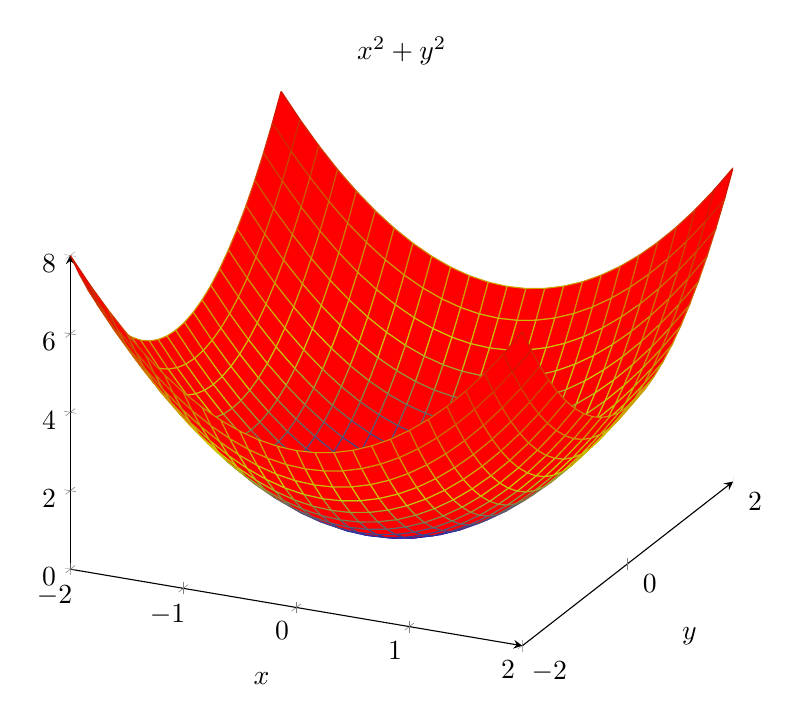
\begin{tikzpicture}
\begin{axis}[
	title=\(x^2+y^2\),
	axis lines = left,
	xlabel=\(x\),
	ylabel={\(y\)},
	xmin=-2, xmax=2,
	ymin=-2, ymax=2,	
]
\addplot3[surf,domain=-2:2, color=red,]{x^2+y^2};

\end{axis}
\end{tikzpicture}
}

\dfn{Nivåkurvor}
{
En nivårkurva till en reellvärd funktion $ f $ av 2 variabler består av alla punkter $ (x,y) $ i definitionsmängden till $ f $ som uppfyller en evkation $ f(x,y) = C $ för något fixt tal $ C $. Detta är i många fall en kurva.\\\\

Tänk på en topografiska kartor! Nivåkurvor är då höjdkurvor, d.v.s. kurvor längs vilka höjden är konstant.\\\\

Vi kan också tänka på en nivåkurva av en funktion av tre variabler: punkter $ (x,y,z) $ så att $ f(x,y,z) = C $ för något fixt tal $ C $. Detta är i många fall en yta.  
}

\ex{}
{
	Om $ f(x,y) = x^2+y^2 $ så ges nivåkurvorna $ \{ (x,y) : x^2+y^2 = C \} $. $ C > 0: $ cirkel med radie $ \sqrt{C}  $. Om $ C = 0: \: (0,0) $. Om $ C < 0: \: $ så finns det inte såna punkter.    
}

\nt{Nivåkurvan är projiceringen till xy-planet av den kurva vi får om vi skär funktionsgrafen med planet $ z = C $ }

\pagebreak
\qs{}
{
Låt $ f(x,y) = x^2y $. Bestäm definitionsmängden till $ f $. Rita nivåkurvorna $ f(x,y) = 1 $ och $ f(x,y) = -1 $.
}
\sol $ D_f $ är $ \mathbb{R}^2 $

\vspace{20pt}
\nt{Samma kurva i $ \mathbb{R}^2 $ kan beskrivas på flera olika sätt: T.ex som nivåkurva, funktionskurva, parameterkurva }
\ex{}
{
Parabel $ y = x^2 $ ges av:
\begin{itemize}
	\item En nivåkurva till funktionen $ f(x,y) = x^2-y $
\end{itemize}
}

\ex{}
{
Paraboloiden kan beskrivas $ z = x^2+y^2 $ t.ex som:
\begin{itemize}
	\item En nivåkurva till funktionen $ f(x,y,z) = x^2+y^2-z^2 $
	\item $ z = r^2 $ i cyllindriska koordinater
	\item Parametriseringarna
\end{itemize}
}

\dfn{Gränsvärdet för funktioner $ \mathbb{R}^n \to \mathbb{R} $ }
{
En reellvärd funktion $ f $ av $ n $ variabler sägs ha gränsvärdet $ L $ när $ x $ går mot $ a $, skrivet:
\begin{equation*}
\lim_{x \to a} f(x) = L
\end{equation*}
Om det för varje tal $ \epsilon > 0 $ finns ett tal $ \delta > 0 $ så att:
\begin{equation*}
0 < |x-a| < \delta \implies  |f(x)-L| < \epsilon
\end{equation*}
Förutsatt att $ x $ tillhör definitionsmängden för $ f $. I ovanstående definition förutsätter vi att varje omgivning av $ a $ innehåller punkter från definitionsmängden till $ f $ (skillda från $ a $)
}

\dfn{Kontinuitet för funktioner $ \mathbb{R}^n \to \mathbb{R} $ }
{
En reelvärd funktion $ f $ av $ n $ variabler är kontinuerlig i en punkt $ a $ om:
\begin{equation*}
\lim_{x \to a} f(x) = f(a)
\end{equation*}
Om detta gäller för alla punkter i definitionsmängden sägs $ f $ vara en \textbf{kontinuerlig funktion}. Detta betyder att man ska få samma gränsvärde oavsett vilken väg man tar till punkten $ a $. \\\\

\textbf{Ex}: Om $ n = 2 $ och punkten har koordinater $ (a,b) $ betyder detta:
\begin{equation*}
	\lim_{(x,y) \to (a,b)} f(x,y) = f(a,b)
\end{equation*}
}

\pagebreak
I \textbf{flervariabeln} är det mer komplicerat när det kommer till kontinuiteten av en funktion. Vi har oändligt många riktningar. Gränsvärdet längs alla kurvor måste sammanfalla och vara lika med funktionsvärdet.

\ex{}
{
\begin{align*}
	f(x,y) &= \frac{x}{ \sqrt{x^2+y^2} }, \: (x,y) \ne (0,0)\\
	f(x,y) &= 0, \: \text{annars} 
\end{align*}
Att $ f $ är kontinuerlig i $ (0,0) $ innebär att funktionsvärdet i $ (x,y) $ närmar sig $ (0,0) $  så fort $ (x,y) $ närmar sig $ (0,0) $.\\\\

Om $ y = 0 $ får vi att:
\begin{equation*}
f(x,0) = \frac{x}{ \sqrt{x^2} } 
\end{equation*}
...som i sin tur ger en värde av +1 om $ x > 0 $ och en värde av -1 om $ x < 0 $. Alltså man kan se redan nu att gränsvärdet existerar ej:
\begin{equation*}
\lim_{(x,y) \to (0,0)} f(x,y)
\end{equation*}
Kraven för kontinuitet är att gränsvärdet ska existera \textbf{och} vara lika med funktionsvärdet. Första kraven på existensen av gränsvärdet misslyckas.
}

\qs{}
{
Funktionen
\begin{align*}
	f(x,y) &= \frac{xy}{x^2+y^4}, \: (x,y) \ne (0,0)\\
	f(x,y) &= 0, \: (x,y) = (0,0)
\end{align*}
...uppfyller:
\begin{align*}
	\lim_{(x,0) \to (0,0)} f(x,0) &= \lim_{(0,y) \to (0,0)} f(0,y) = f(0,0) = 0
\end{align*}
D.v.s., gränsvärdet då $ (x,y) \to (0,0) $ längs linjerna $ y = 0 $ och $ x = 0 $ är 0 som är lika med funktionsvärdet. Är den kontinuerlig? Varför? Varför inte?
}
\sol De givna gränsvärden säger att gränsvärderna längs koordinataxlarna är lika med 0. Men $ f(x,x)  $ då $ x \to 0 $ går mot $ 1 $, alltså funktionen är diskontinuerlig eftersom gränsvärdet stämmer inte överens med funktionens värde.

\vspace{20pt}
\nt{Kontinuitet bevaras av de fyra räknesätten och sammansättning. \textbf{Elementära} utryck (exp, log, sin, cos, tan, cot, arcsin, arccos, arctan, polynom, rationella utrcuk, pot, samt abs).}
Att beräkna gränsvärden (närde existerar) är generellt mycket svårare än att visa att de inte har gränsvärden (när den inte existerar).\\\\

\pagebreak
\ex{Beräkna gränsvärdet}
{
\begin{equation*}
\lim_{(x,y) \to (0,0)} \frac{x^2+y^4}{ \sqrt{4x^2+4y^2}  } 
\end{equation*}
Vi vill undersöka om gränsvärdet existerar. Vi först testar längs axlarna:
\begin{align*}
	f(x,0) &= \frac{x^2}{ \sqrt{4x^2} } = \frac{1}{2} |x| \to 0, \: x \to 0\\
	f(0,y) &= \frac{y^4}{ \sqrt{4y^2} }   \frac{1}{2} |y^3| \to 0, \: y \to 0
\end{align*}
Vi satsar på att gränsvärdet finns. Vi inför $ x = rcos\theta, \: y = rsin\theta \implies \sqrt{4x^2+4y^2} = 2 \sqrt{x^2+y^2} = 2r$. $ x^2+y^2 = r^2 $:
\begin{equation*}
	f(x,y) = \frac{x^2+y^2}{ \sqrt{4x^2+ry^2} } = \frac{r^2cos^2\theta + r^4sin^4\theta}{2r} = \frac{1}{2} ( rcos^2\theta + r^3sin^4\theta ) \to 0, \: r \to 0 
\end{equation*}
Eftersom $ r \to 0 \iff (x,y) \to (0,0) $ betyder det att:
\begin{equation*}
\lim_{(x,y) \to (0,0)} f(x,y) = 0
\end{equation*}
En intuitiv tankesätt med att man byter till polära koordinater är att man kollar att varje punkt i cirkeln med centerpunkten i $ (0,0) $ har samma gränsvärdet medan radien för cirkeln går också mot 0. Alltså på det sättet man bevisar att alla punkter runt (och inte bara koordinataxlarna) går mot 0.
}

\pagebreak
\chapter{Modul 2}
\section{Föreläsning 4 (28/03/2023)}
Partiella derivator,

\dfn{Partiella derivator}
{
Om $ f = f(x,y) $ är en reellvärd funktion av 2 variabler så definieras de partiella derivatorna av $ f $ i punkten $ (a,b) $ i definitionsmängden genom:
\begin{align*}
	\frac{\partial}{\partial x}(a,b) &= \lim_{h \to 0} \frac{f(a+h,b)-f(a,b)}{h}\\
\frac{\partial}{\partial y}(a,b) &= \lim_{k \to 0} \frac{f(a,b+k)-f(a,b)}{k} 
\end{align*}
...under förutsättning att dessa gränsvärden existerar.\\\\

Om funktionen beror på fler än 2 variabler definieras de partiella derivatorna med avseende på alla dessa variabler på liknande sätt. Många olika beteckningar. 
}

\ex{Om $ f(x,y) = x^2+y^2 $ bestäm $ \frac{\partial f}{\partial x} (1,1) $ }
{
Vi inför $ g(x) = f(x,1) = x^2+1 $. Då får vi $ \frac{\partial f}{\partial x} (1,1) = g'(1) = 2x,\: x = 1 \implies 2 $  
}

\dfn{ $ \nabla f $ (nabla av $ f $ )}
{
Det är också praktiskt att införa notationen för $ f $ som beror av $ x $ och $ y $:
\begin{equation*}
\nabla f = \Bigl( \frac{\partial f}{\partial x}, \frac{\partial f}{\partial y} \Bigr)
\end{equation*}
Detta kan tolkas som vektorn som pekar mot punkten i kurvan som håller på att minimeras.
}

\ex{ $ f(x,y) = x^2y+y^3 $ }
{
\begin{itemize}
	\item 1) $ \frac{\partial f}{\partial x} = \frac{\partial}{\partial x}(x^2y) + \frac{\partial}{\partial x}(y^3) = 2xy + 0 = 2xy$
	\item 2) $ \frac{\partial f}{\partial y} = \frac{\partial}{\partial y}(x^2y) + \frac{\partial}{\partial y}(y^3) = x^2+3y^2 $ 
\end{itemize}
}

\ex{ $ g(x,y,z) = x^2yz^3 $  }
{
\begin{itemize}
	\item $ \frac{\partial g}{\partial x} = \frac{\partial}{\partial x} (x^2yz^3) = 2xyz^3 $
	\item $ \frac{\partial g}{\partial y} = \frac{\partial}{\partial y}(x^2yz^3) = x^2z^3 $
	\item $ \frac{\partial g}{\partial z} = \frac{\partial}{\partial z}(x^2yz^3) = 3x^2yz^2$ 
\end{itemize}
}

\qs{}
{
Om $ f(x,y) = \sqrt{1+xy}  $, beräkna $ \frac{\partial f}{\partial y} (2,1) $ 
}

\sol $ \frac{\partial f}{\partial x} = \frac{1}{2 \sqrt{1+xy} } \cdot \frac{\partial}{\partial y}(1+xy) = \frac{1}{2 \sqrt{1+xy} } \cdot x   $. (2,1) $ \implies \frac{1}{ \sqrt{3} }  $  

\vspace{20pt}
\qs{}
{
Om $ h(x,y) = arctan\bigl( \frac{y}{x} \bigr) $, beräkna $ \frac{\partial h}{\partial x} ( \sqrt{3} , 1)$  
}
\sol:
\begin{equation*}
\frac{\partial h }{\partial x} = \frac{1}{ \frac{x^2}{y^2} +1} \cdot - \frac{y}{x^2}   
\end{equation*}
$ (x,y) = ( \sqrt{3} ,1) \implies \frac{1}{4} \cdot - \frac{1}{3} = - \frac{1}{12}  $ 

\vspace{20pt}
\subsection{Inledning till tangentplan}
\ex{}
{
Finn en parametrisering av kurvan som är skärningen av ytan $ z = x^2+y^2 $ med planet $ y = 1, \: x = 2 $. Bestäm en tangentvektor till denna kurva i punkten $ (2,1,5) $. Sen med hjälp av linjär algebra, bestäm ekvationen för det plan genom punkten $ (2,1,5) $ som är parallellt med både tangentvektorerna ovan.\\\\

a) Skärningen av $ z = x^2+y^2 $ med planet $ y = 1 $ ges då av $ \{ y = 1, \: z = x^2+1, \: x \in \mathbb{R} \} $. En parametrisering av kurvan är då $ \vec{r} (x) =  (x,1,x^2+1), \: x \in \mathbb{R} $. Vi ser att $ x = 2 $ svarar mot $ (2,1,5) $. En tangentvektor till kurvan i $ (2,1,5) $ ges av $ \vec{r}' (2) $.
\begin{equation*}
\vec{r} '(x) = (1, 0, 2x),\: \vec{r} ' (2) = (1,0,4)
\end{equation*}
\noindent
b) Skärningen med planet $ x = 2 $, ges av $ \{ x = 2, \: z = 4+y^2, \: y \in \mathbb{R} \} $. Den parametriseras av $ \vec{s} (y) = (2,y,4+y^2), \: y \in \mathbb{R} $. Vi ser att $ \vec{s} (1) = (2,1,5) $. En tangentvektor till kurvan i $ (2,1,5) $ ges av:
\begin{equation*}
\vec{s} ' (y) = (0,1,2y), \: \vec{s} '(1) = (0,1,2)
\end{equation*}
\noindent
c) Vi söker planet som innehåller punkten $ (2,1,5) $ och som är parallelt med $ (1,0,4) $ och $ (0,1,2) $. Alltså har planet en normal som är ortogonal mot de här vektorerna. Normalen tas fram genom kryssprodukten:
\begin{equation*}
\begin{pmatrix}
	1 \\
	0 \\
	4 \\
\end{pmatrix}
\times
\begin{pmatrix}
	0 \\
	1 \\
	2 \\
\end{pmatrix}
=
\begin{pmatrix}
	-4 \\
	-2 \\
	1 \\
\end{pmatrix}
\end{equation*}
Planet ges då av $ (-4,-2,1) \cdot (x-2,y-1,z-5) = 0 $ som kan förlänga om man vill. 
}

Vad gjorde vi? $ f(x,y) = x^2+y^2 $. $ T_x = (1,0,4),\: T_y = (0,1,2) $. Vi bestämmer:
\begin{align*}
	\frac{\partial f}{\partial x} &= 2x, \: (x,y) = (2,1) \implies 4\\
	\frac{\partial f}{\partial y} &= 2y, \: (x,y) = (2,1) \implies 2
\end{align*}
Alltså: $ T_x = (1,0, \frac{\partial f}{\partial x} ), \: T_y = (0,1, \frac{\partial f}{\partial y} )$. En vektor ortogonal mot dessa är: $ ( \frac{\partial f}{\partial x} , \frac{\partial f}{\partial y}, -1) $. Ekvationen för planet ges då av:
\begin{equation*}
	( \frac{\partial f}{\partial x}, \frac{\partial f}{\partial y}, -1 ) \cdot ( x-2,y-1, z-f(2,1) ) = 0 \implies \frac{\partial f}{\partial x} (x-2) + \frac{\partial f}{\partial y} (y-1) - (z - f(2,1)) = 0
\end{equation*}
Tangentlinjen för $ g(x) $ i $ x_0 $:
\begin{equation*}
y = g(x_0) + g'(x_0)( x-x_0 )
\end{equation*}

\dfn{Tangentplan}
{
Om $ f $ uppfyller dessa villkor så ges tangentplan i punkten $ (a,b, f(a,b)) $ till funktionsytan $ z = f(x,y) $ av ekvationen:
\begin{equation*}
z = f(a,b)+ \frac{\partial f}{\partial x}(a,b)(x-a) + \frac{\partial f}{\partial y}(y-b)
\end{equation*}
}

\vspace{20pt}
\qs{}
{
Bestäm en ekvation för tangentplanet i punkten $ (1,2,3) $ till funktionsytan $ z = f(x,y) $ om $ f(x,y) = x^2y+y^3-7 $ 
}
\sol 
\begin{align*}
	\frac{\partial f}{\partial x} &= 2xy, \: \frac{\partial f}{\partial x}(1,2) = 4\\
	\frac{\partial f}{\partial y} &= x^2+3y^2, \: \frac{\partial f}{\partial y}(1,2) = 13
\end{align*}
Planet enligt definition 2.1.3 ges av:
\begin{equation*}
z = 3 + 4(x-1) + 13(y-2)
\end{equation*}

\vspace{20pt}
\noindent
Om $ f = f(x,y) $ är partiellt deriverbar så är de partiela derivatorna nya funktioner av $ x $ och $ y $. Vi kan förstås undra om dessa funktioner är partiellt deriverbara. I så fall får vi andra ordningens partiella derivator till $ f $. Det finns fyra möjligheter:
\begin{equation*}
\frac{\partial^2 f}{\partial x^2}, \: \frac{\partial^2 f}{\partial y \partial x}, \: \frac{\partial^2 f}{\partial x \partial y}, \: \frac{\partial^2 f}{\partial y^2}
\end{equation*}

\pagebreak
\ex{}
{
Vi har $ \frac{\partial f}{\partial x} = 2xy, \: \frac{\partial f}{\partial y} = x^2+3y^2 $:
\begin{align*}
	\frac{\partial^2 f}{\partial x^2} &= \frac{\partial}{\partial x}(2xy) = 2y\\
	\frac{\partial^2 f}{\partial y \partial x} &= \frac{\partial}{\partial y}(2xy) = 2x\\
	\frac{\partial^2 f}{\partial y^2} &= \frac{\partial}{\partial y}(x^2+3y^2) = 6y\\
	\frac{\partial^2 f}{\partial x \partial y} &= \frac{\partial}{\partial x}(x^3+3y^2) = 2x
\end{align*}
}

\ex{}
{
Avgör om ytan $ f(x,y) = z = x^2+4xy-2y^2+12x-12y-1 $ har någon tangentplan som är horisontellt (d.v.s parallelt med xy-planet). Finn i så fall ekvationen för detta tangentplan och den punkt där planet tangerar ytan.\\\\

\textbf{Fråga}: Har funktionsytan något tangentplanet som är parallellt med xy-planet?\\\\

Om ett tangentplan är paralellt med xy-planet så är normalen parallell med z-axeln. Tangentplanet beskrivs av:
\begin{equation*}
\frac{\partial f}{\partial x} \cdot (x-a) + \frac{\partial f}{\partial y} \cdot (y-b) - (z-f(a,b)) = 0
\end{equation*}
Normalen, $ ( \frac{\partial f}{\partial x}, \frac{\partial f}{\partial y}, -1  ) $. Att normalen är parallell med z-axeln betyder att $ \frac{\partial f}{\partial x} = \frac{\partial f}{\partial y} = 0$ i något punkt. Frågan är alltså om det finns $ (a,b) $ så att $ \frac{\partial f}{\partial x}(a,b) = \frac{\partial f}{\partial y}(a,b) = 0 $. Vi räknar:
\begin{align*}
	\frac{\partial f}{\partial x} &= 2x-4y+12, \:\: (1)\\ 
	\frac{\partial f}{\partial y} &= -4x-4y-12 = 0 \:\: (2)
\end{align*}
$ (1)-(2) \implies 2x+12+4x+12 = 0 \iff 6x = -24 \iff x = -4 $. Genom att sätta den i $ (1) $ så får man att $ -8 -4y + 12 = 0 \iff 4y = 4 \iff y = 1 $.\\\\

\textbf{Svar}: Ja en sådan punkt existerar och ges av $ (-4,1,f(-4,1)) = (-4,1,-31) $. Tangentplanen ges alltså då av $ z = -31 $ eftersom andra partiellderivatorna försvinner (= 0) 
}

\vspace{20pt}
\noindent
I envariabeln så kunde vi göra linjär approximation med hjälp av tangentlinjen så fort funktionen var differentierbar (derivatan existerar). Deriverbarhet implicerar också kontinuitet.\\\\

\noindent
I flervariabeln är det lite mer komplicerat. Att en funktion har partiella derivator betyder nödvändigtvis inte att funktionen är kontinuerlig eller att den kan approximieras av tangentplanet. Därmot finns ett begrepp som är differentierbarhet som säger exakt detta. Det räcker också om vi kan säga att de partiella derivatorna är kontinuerliga


\ex{}
{
Om $ f(x,y) $ definieras som följande:
\begin{align*}
	f(x,y) &= \frac{xy}{x^2+y^4}, \: (x,y) \ne (0,0)\\
	f(x,y) = (0,0), \: (x,y) = (0,0)
\end{align*}
$ f(0,y) = f(x,0) = 0 $. Alltså $ \frac{\partial f}{\partial x} (0,0) = \frac{\partial f}{\partial y}(0,0) =  0	$. Men $ f $ var ej kontinuerlig. 
}

\pagebreak
\section{Föreläsning 5 (29/03/2023)}
Vektorfält

\dfn{Vektorfält}
{
	Ett vektorfält är en funktion $ F $ definierad i någon delmängd av $ \mathbb{R}^3 $ med funktionsvärden i $ \mathbb{R}^3 $. Motsvarande i $ \mathbb{R}^2 $ kallas plana vektorsfält. Det är helt enkelt en funktion från $ \mathbb{R}^3 $ till $ \mathbb{R}^3 $, vilket vi då kan se som tre funktioner från $ \mathbb{R}^3 $ till $ \mathbb{R} $.\\\\

\textbf{Tolkning}: I varje punkt $ (x,y,z) $ sitter en vektor $ F(x,y,z) $
}

\ex{Vektorfäktet $ G(x,y) = (-y, 0) $ }
{
Vi tittar på $ G $ i några punkter:
\begin{align*}
	G(0,0) &= (0,0), \: G(1,0) = (0,0), \: G(-1, 0) = (0,0)\\
	G(0,1) &= (-1,0), \: G(1,1) = (-1,0), \: G(-1,1) = (-1,0) \\
	G(0,-1) &= (1,0), \: G(1,01) = (1,0), \: G(-1,-1) = (1,0)
\end{align*}
}

\ex{}
{
Ett annat exempel på vektorfält är:
\begin{equation*}
\nabla f(x,y) = \Bigl( \frac{\partial f}{\partial x}(x,y), \: \frac{\partial f}{\partial y}(x,y)  \Bigr)
\end{equation*}
Om $ f = f(x,y) $ 
}

\noindent
\textbf{Varför vektorfält?}:
\begin{itemize}
	\item Kraftfält: Gravitationsfält, elektriskt kraftfält:
	\begin{equation*}
		F = c\Bigl( -\frac{x}{ \sqrt{x^2+y^2+z^2}  }, \: - \frac{y}{ \sqrt{x^2+y^2+z^2} }, \: - \frac{z}{ \sqrt{x^2+y^2+z^2} }     \Bigr)
	\end{equation*}
	\item Magnetfält kring en ledare
	\begin{equation*}
	F = c \Bigl( - \frac{y}{x^2+y^2}, \: - \frac{x}{x^2+y^2}    \Bigr)
	\end{equation*}
	\item Arbete: Integraler av vektorfält längs kurvor 
\end{itemize}

\dfn{Strömlinjer, Fältlinjer (obs många andra namn finns)}
{
En kurva till vilken vektorfält är tangentiellt i varje punkt kallas en strömlinje (fältlinje, flödeslinje, trajektoria, integralkurva). Om $ F(x,y) = (P, Q) $ är ett plant vektorfält fås fältlinjerna som lösningar till:
\begin{equation*}
\frac{dx}{P} = \frac{dy}{Q} 
\end{equation*}
På liknande sätt fås strömlinjerna i 3D. Om kurvan kan parametriseras som $ r(t) $ så gäller:
\begin{equation*}
r'(t) = \lambda (t) F(r(t)) = \lambda (t) (P(r(t)), Q(r(t)), R(r(t)))
\end{equation*}
En strömlinje är en kurva vars tangent i en punkt $ (x,y) $ är proportionell mot vektorfältet $ F(x,y) $. Om kurvan ges av $ (x, y(x)) $ då ges tangentens riktning av $ (a, \frac{dy}{dx} ) $. Om det är en strömlinje så får vi $ (1, \frac{dy}{dx} ) = \lambda(x) F(x,y) $ 
}

\ex{Hitta strömlinjerna till vektorfältet $ F(x,y) = (-y,1) $ }
{
Vi evaluerar $ F $ i några punkter:
\begin{align*}
F(1,0) = (0,1), \: F(1,1) = (-1,1), \: F(1,-1) = (1,1)
\end{align*}

Här $ P = -y $ och $ Q = 1 $:
\begin{equation*}
\frac{dy}{dx} = - \frac{1}{y} \iff \frac{dx}{dy} = -y \implies x(y) = -\frac{y^2}{2} + C  
\end{equation*}
Alltså detta kan se ut som horisontella parabelkurvor 
}

\qs{}
{
Finns strömlinjerna till hastighetsfältet $ H(x,y) = (-y,x) $
}
\sol 
\begin{equation*}
	-\frac{dx}{y} = \frac{dy}{x} \iff -\int_{}^{} x \: dx = \int_{}^{} y \: dy = -x^2 + C = y^2 \iff x^2+y^2 = C  
\end{equation*}

\vspace{20pt}

\dfn{Konservativa vektorfält}
{
Om det finns en funktion $ \phi $ sådan att $ \nabla\phi = F $ så sägs vektorfältet $ F $ vara konservativt. Funktionen $ \phi $ kallas i så fall för en potentialfunktion till $ F $. 

\begin{itemize}
	\item Om $ F = F(x,y), \: \nabla\phi (x,y) = \Bigl( \frac{\partial \phi}{\partial x}(x,y), \: \frac{\partial \phi(x,y)}{\partial y} \Bigr) = (P,Q)$. Så då är $ F $ konservativ om $ \frac{\partial \phi}{\partial x} = P, \: \frac{\partial \phi}{\partial y} = Q $
	\item Om $ F(P, Q,R)  $ så är $ F $ konservativ om $ \frac{\partial \phi}{\partial x} = P, \: \frac{\partial \phi}{\partial y} = Q, \: \frac{\partial \phi}{\partial z} = R$ 
\end{itemize}
}

\ex{}
{
Är $ \phi = arctan(xy) $ en potential funktion til:
\begin{equation*}
F(x,y) = \Bigl( \frac{x}{1+x^2y^2} , \: \frac{y}{1+x^2y^2}   \Bigr)
\end{equation*}
\begin{equation*}
\frac{\partial \phi}{\partial x} = \frac{1}{1+x^2y^2} \cdot y \ne \frac{x}{1+x^2y^2} 
\end{equation*}
(Förutom i origo). Alltså $ \phi $ kan ej vara en potentialfunktion till $ F $
}

\ex{Är $ F(x,y) = (x,y) $ konservativt?	}
{
	Vi försöker hitta potentiella funktionen $ \phi $, d.v.s. $ \phi $ som uppfyller:
\begin{align}
		\frac{\partial \phi}{\partial x} &= x\\
	\frac{\partial \phi}{\partial y} &= y
\end{align}
(2.1) implicerar att $ \phi (x,y) = \frac{x^2}{2} + h(y) $. $ \frac{\partial \phi}{\partial y} = \frac{\partial}{\partial y} \Bigl( \frac{x^2}{2} + h(y) \Bigr)  = h'(y) = y \implies h(y) = \frac{y^2}{2} + C$. Alltså $ \phi (x,y) = \frac{x^2}{2} + \frac{y^2}{2} +C $ är potentialfunktionen till $ F $. Alltså så är $ F $ \textbf{konservativt}.   
}

\nt{ \textbf{Nödvändig villkor} för att testa för konservatism:
Om $ F = (P,Q) $ är konservativt så:
\begin{equation*}
P = \frac{\partial \phi  }{\partial x } , \: Q = \frac{\partial \phi  }{\partial y }   
\end{equation*}
 Vi vet att $ \frac{\partial^2 \phi  }{\partial xy } = \frac{\partial^2 \phi  }{\partial yx } \implies \frac{\partial Q }{\partial x } = \frac{\partial P }{\partial y }   $ 
}

\ex{}
{
$ F(x,y) = (x,y) $, $ P = x $, $ Q = y $. Vi har att:
\begin{equation*}
\frac{\partial Q }{\partial x } = \frac{\partial P }{\partial y } = 0
\end{equation*}
Det betyder att $ F $ \textbf{kan} vara konservativt
}

\ex{}
{
$ F(x,y) = (-y,1) $, $ P = -y $, $ Q = 1 $. Vi har att:
\begin{equation*}
\frac{\partial P }{\partial y } = -1, \: \frac{\partial Q }{\partial x } = 0 
\end{equation*}
Alltså kan $ F $ \textbf{ej} vara konservativt.
}

\qs{}
{
Är hastighetsfältet $ H(x,y) = (-\omega y, \omega x) $ konservativt?
}

\sol 
1) $  P = -\omega y, \: Q = -\omega x \implies \frac{\partial Q }{\partial x } = \omega, \: \frac{\partial P }{\partial y } = -\omega $. Om $ \omega \ne 0$ så är de inte samma. Det betyder att om $ \omega \ne 0 $ så är $ H $ ej konservativt. Om $ \omega = 0 $ så är $ H $ triviellt konservativt.  \\\\

\noindent
2) \begin{equation*}
\frac{\partial \phi }{\partial  x} = - \omega y, \: \frac{\partial \phi  }{\partial y } = \omega x 
\end{equation*}
$ (1) \implies \phi (x,y) = - \omega xy + h(y) $. Insatt i $ (2) $: $ \frac{\partial \phi  }{\partial y } = - \omega x + h'(y) = \omega x \implies h'(y) = 2\omega x $ som är ej möjligt om $ \omega \ne 0 $. Alltså ej konservativ om $ \omega \ne 0 $ 

\pagebreak
\section{Föreläsning 6 (30/03/2023)}
Kurvintegraler.\\\\

\dfn{Längden av en parametriserad kurva}
{
Längden av en parametriserad kurva $ \gamma $ som ges av $ r(t) $, $ a \le t \le b $ räknade vi ut som:
\begin{equation*}
L = \int_{ \gamma}^{}  \: ds = \int_{a}^{b} |r'(t)| \: dt 
\end{equation*}
Detta definierades som gränsvärdet av Riemannsummor:
\begin{equation*}
\sum_{}^{} |\Delta r_j|
\end{equation*}
Vi ska nu titta mer allmänt på integraler av den här typen där vi även har en integrand.
}
\dfn{Kurvintegraler (linjeintegraler)}
{
Låt $ \gamma $ vara en begränsad, slät kurva i $ \mathbb{R}^3 $ (eller $ \mathbb{R}^2 $ ) och $ f $ någon funktion som är definierad och kontinuerlig på $ \gamma $, Då kan vi definiera kurvintegraler som:
\begin{equation*}
\int_{ \gamma}^{} f(x,y,z) \: ds 
\end{equation*}
...som gränsvärdet av Riemannsummor:
\begin{equation*}
\sum_{}^{} f(x_j*, y_j*, z_j*) | \Delta r_j|
\end{equation*}
\begin{align*}
	x &= x(t)\\
	y &= y(t)\\
	z &= z(t)
\end{align*}
$ t \in I $ medför:
\begin{equation*}
\int_{I}^{} f(x(t),y(t),z(t)) \sqrt{(x')^2+(y')^2+(z')^2}  \: dt 
\end{equation*}
Alltså kurvintegralen kan beräknas genom:
\begin{equation*}
\int_{ \gamma}^{} f(x,y,z) \: ds = \int_{a}^{b} f(r(t)) |r'(t)|\: dt  
\end{equation*}
..där $ r(t) $ , $ a \le t  \le b$ är en parametrisering av $ \gamma $. 
}

\ex{}
{
Beräkna kurvintegralen som begränsas av $ y $ och första delen av halvcirkeln:
\begin{equation*}
\int_{ \gamma}^{} y \: ds 
\end{equation*}

\textbf{Lösning}: Vi kan parametrisera $ \gamma $ (övre delen av halvcirkeln) enligt:
\begin{align*}
x(t) = cos(t)\\
y(t) = sin(t), \:\: t \in [0,\pi)
\end{align*}
Vi har $ x'(t) = -sint, \: y'(t) = cost $:
\begin{equation*}
\implies \sqrt{(x')^2+(y')^2} = \sqrt{sin^2t+cos^2t} = 1
\end{equation*}
Här är $ f(x,y) = y $ och i en punkt $ (x(t), y(t)) $ är detta $ y(t) = sint $. Alltså ges integralen av:
\begin{equation*}
	\int_{0}^{ \pi} sint \: dt = \bigl[ -cost \bigr]_0^{ \pi } = cos0 - cos\pi = 2 
\end{equation*}
}

\dfn{Kurvintegraler av vektorfält}
{
Om $ F = (P,Q) $ är ett kontinuerligt plant vektorfält och $ \gamma $ em orienterad slät kurva så ges kurvintegralen av den tangentiella komponenten av $ F $ längs $ \gamma $ av:
\begin{equation*}
\int_{ \gamma}^{} F \cdot  dr = \int_{ \gamma}^{} P \: dx + \int_{ \gamma}^{} Q \: dy   
\end{equation*}
Om $ r(t) = (x(t), y(t)) $ , $ a \le t \le b $ parametriserar $ \gamma $ så kan kurvintegralen beskrivas genom:
\begin{equation*}
\int_{a}^{b} (P(x(t),y(t))x'(t) + Q(x(t),y(t))y'(t) \: dt 
\end{equation*}
...detta kan göras motsvarande för vektorfält i $ \mathbb{R}^3 $ 
}

\pagebreak
\ex{Exempel på kurvintegraler av vektorfält}
{
Beräkna kurvintegralen:
\begin{equation*}
\int_{ \gamma}^{} F \cdot  dr
\end{equation*}
\begin{itemize}
	\item A) Om $ F(x,y) = (x,-y) $ och $ \gamma $ är den del av kurvan $ y = 1 -x^2 $ som ligger i första kvadranten, genomlöpt från (1,0) till (0,1)
	\item B) Om $ F(x,y) = (x,-y) $ och $ \gamma $ är den del av enhetscirkeln som ligger i första kvadranten, genomlöpt från $ (1,0) $ till $ (0,1) $
\end{itemize}

\textbf{A)}\\
Vi kan parametrisera $ \gamma $ enligt:
\begin{align*}
	x &= x\\
	y &= 1 -x^2,\:\: x : 1 \to 0
\end{align*}
$ \vec{r} (t) = (x,1-x^2) $. TV $ \vec{r} '(t) = (1,-2x), \: F( \vec{r} (t))  = (x,x^2-1) $. Kurvintegralen ges av:
\begin{equation*}
\int_{1}^{0} F( \vec{r} (x)) \cdot \vec{r} '(x) \: dx = \int_{1}^{0} x - 2x^3+2x \: dx  
\end{equation*}
\begin{equation*}
	\int_{0}^{1} 3x-2x^3 \: dx \bigl[ \frac{3x^2}{2} - \frac{2x^4}{4}  =  \bigr]_{1}^{0} = \frac{1}{2} - \frac{3}{2} = -1
\end{equation*}
\textbf{B)} \\
Vi kan parametrisera denna del av enhetscirkeln som:
\begin{align*}
F(t) = (cos(t), sin(t)), \: t : 0 \to \frac{\pi}{2} 
\end{align*}
$ F'(t) = (-sint, cost), \: F( \vec{r} (t)) = (cost, -sint), \: F( \vec{r}(t)) \cdot \vec{r} (t) = -2sintcost = -sin2t  $.
\begin{equation*}
	\int_{0}^{ \frac{\pi}{2} } - sin2t \: dt = \bigl[ \frac{cos2t}{2}   \bigr]_{0}^{ \frac{\pi}{2}  } = -1
\end{equation*}

}

\dfn{Kurvintegraler av konservativa vektorfält}
{
Om $ F $ är ett konservativt vektorfält med potentialfunktionen $ \phi  $ och $ \gamma $ är en orienterad slät kurva som startar i $ (x_0, y_0) $ och slutar i $ (x_1, y_1) $ så gäller att:
\begin{equation*}
\int_{ \gamma}^{} F \cdot dr = \phi ( x_1, y_1 ) - \phi (x_0, y_0) 
\end{equation*}
\textbf{Motivierign}: Om,
\begin{equation*}
	\gamma := (x(t), y(t)), \: t \in [t_0, t_1]
\end{equation*}
$ \phi  $ längs $ \gamma $: $ \phi (x(t), y(t)) $.
\begin{equation*}
\frac{d}{dt} \phi (x(t), y(t)) = \frac{\partial \phi  }{\partial x } x'(t) + \frac{\partial \phi  }{\partial y } y'(t)
\end{equation*}
Alltså är $ \phi (x(t), y(t)) $ en primitiv funktion till $ \nabla \phi \cdot (x'(t),y'(t)) $:
\begin{equation*}
\implies \int_{}^{} \nabla \phi \cdot (x'(t),y'(t)) \: dt = \phi (x(t_1),y(t_1))- \phi (x(t_0), y(t_0)) 
\end{equation*}
}

\qs{}
{
\textbf{Möjligt tentaproblem}:
Betrakta det plana vektorfältet $ F $ som ges av:
\begin{equation*}
F(x,y) = \bigl( x+ \frac{y}{2} +3, \frac{x}{2} +y+5 \bigr)
\end{equation*}
\begin{itemize}
	\item A) Visa att vektorfältet är konservativt
	\item B) Använd vetskapen att vektorfältet är konservativt för att beräkna kurvintegralen
	\begin{equation*}
	\int_{ \gamma}^{} F \cdot dr = \int_{ \gamma}^{} x+  \frac{y}{2} + 3 \: dx + \int_{ \gamma}^{} \frac{x}{2} +y+5 \: dy   
	\end{equation*}
	...där $ \gamma $ är någon slät kurva som börjar i $ (-2,0) $ och slutar i $ (-2,-4) $ 
\end{itemize}
}
\sol A)
\begin{align*}
	\phi &= ( \frac{x^2}{2} + \frac{xy}{2} + 3x + \frac{y^2}{2} +5y)\\
	\nabla \phi &= (x+ \frac{y}{2} +3, \frac{x}{2}  + y + 5)
\end{align*}
V.S.B!

\sol B)
\begin{equation*}
\int_{ \gamma}^{} F \cdot dr = \phi (-2,0) - \phi (-2,-4) = -4-(-12) = 8 
\end{equation*}

\vspace{20pt}

\thm{}
{
Om $ F = (P,Q)	$ är ett glatt plant vektorfält på en öppen enkelt sammanhägande mängd $ D $, så är följande påståenden ekvivalenta:
\begin{itemize}
	\item $ F $ är konservativt i D
	\item $ \int_{ \gamma}^{} F \cdot dr = 0$ för alal styckvis släta slutna kurvor $ \gamma $ i $ D $ 
	\item Alla kurvintegraler av $ F $ är oberoende av vägen i $ D $
	\item
	\begin{equation*}
	\frac{\partial Q }{\partial x } = \frac{\partial P }{\partial y }
	\end{equation*}
	...i $ D $ 
\end{itemize}
}

\pagebreak
\chapter{Modul 3}
\section{Föreläsning 7 (3/04/2023)}
Kedjeregeln, differentierbarhet, linjärisering.\\\\

\dfn{Linjäriseringen}
{
Linjäriseringen av $ f $ eller den linjära approximationen av $ f $ kring punkten $ (a,b) $ ges av:
\begin{equation*}
f(x,y) \approx f(a,b) + \frac{\partial f }{\partial x } (a,b)(x-a) + \frac{\partial f }{\partial y } (a,b)(y-b)
\end{equation*}
}

\ex{Använd linjär approximation kring $ (1,2) $ för att hitta ett närmevärde till $ f(1.2,1.8) $ då $ f(x,y) = yln(xy-1) $ }
{
\begin{equation*}
f(x,y) \approx f(a,b) + \nabla f(a,b)(x-a,y-b)
\end{equation*}
Linjär approximation i $ (1.2;1.8) $ ges av $ a = 1 $, $ b = 2 $; $ x = 1.2 $, $ y = 1.8 $.
\begin{align*}
	f(1,2) &= 0\\
	\frac{\partial f }{\partial x } &= y \frac{1}{xy-1} \cdot y\\
	\frac{\partial f }{\partial y } &= ln(xy-1) + y \frac{1}{xy-1} \cdot x\\
	\frac{\partial f }{\partial x } (1,2) &= 4\\
	\frac{\partial f }{\partial y }(1,2) &= 2
\end{align*}
$ \implies f(1.2;1.8) \approx 0 - (4,2) \cdot (0.2;-0.2) = 0.4 $ 
}

\dfn{Differentierbarhet $ \mathbb{R}^2 \to \mathbb{R} $ }
{
Funktionen $ f = f(x,y) $ sägs vara differentierbar i en punkt $ (a,b) $ om:
\begin{equation*}
\lim_{(x,y) \to (a,b)} \frac{f(x,y)-f(a,b)- \frac{\partial f }{\partial x } (a,b)(x-a) - \frac{\partial f }{\partial y } (a,b)(y-b)}{ \sqrt{(x-a)^2 + (y-b)^2}   } = 0 
\end{equation*}
Jämför med envariabeldefinitionen. Detta kan tolkas som att tangentplan och linjär approximation fungerar!
}

\noindent
\textbf{Hur vet man om en funktion är differentierbar?}\\
Antingen får man kolla gränsvärdet för hand. Kan vara krångligt. Annars är det ofta enklare:\\\\

\noindent
\textbf{Faktum}: Om $ f $ är kontinuerlig vilket betyder att de partiella derivatorna existerar och är kontinuerliga, i en omgivning av $ (a,b) $, så är $ f $ också differentierbar i $ (a,b) $.

\qs{}
{
	Visa att $ f(x,y) = e^{x^2y-1} $ är differentierbar i $ (-1,1) $. Använd linjär approximation kring $ (-1,1) $ för att hitta ett närmevärde till $ f(-0.5;1.3) $.
}

\sol\\ 
\textbf{A)}  Gradienten är kontinuerliga överallt och enligt satsen är $ f $ differentierbar överallt.\\\\

\noindent
\textbf{B)}
\begin{align*}
	f(-1,1) &= e^{1-1} = 1\\
	\frac{\partial f }{\partial x } (-1,1) &= 2\\
	\frac{\partial f }{\partial y } &= (-1,1) = 1
\end{align*}
Med $ a = -1, \: b = 1, \: x = -0.5 $ och $ y = 1.3 $ får vi:
\begin{equation*}
f(-0.5; 1.3) = f(-1,1) + (-2,1) \cdot  (-0.5-(-1)); 1.3-1) = 1 -2 \cdot 0.5 + 0.3 = 0.3
\end{equation*}
Som är vårt närmevärde av $ f(-0.5, 1.3) $

\thm{}
{
Om $ f $ är differentierbar i en punkt $ (a,b) $ så är $ f $ kontinuerlig i $ (a,b) $  
}

\thm{}
{
Om $ f $ är kontinuerlig, vilket betyder att de partiella derivatorna existerar och är kontinuerliga, i en omgivning av $ (a,b) $ så är $ f $ också differentierbara i $ (a,b) $
}

\nt{Att vara differentierbar betyder inte att partiella derivatorna är kontinuerliga}

\nt{Att ha partiella derivator medför inte differentierbarhet}

\thm{Kedjeregeln i fallet $ \mathbb{R} \to \mathbb{R}^2 \to \mathbb{R} $ }
{
Vi vill derivera sammansättningen $ z = f(x(t), y(t)) $ där $ f(x,y) $ är en funktion av två variabler och $ (x(t), y(t)) $ är en kurva i $ \mathbb{R}^2 $. D.v.s hur ändras $ z $ längs kurvan? Då gäller för $ f $ med kontinuerliga partiella derivator (differentierbarhet) att kedjeregeln blir:
\begin{equation*}
\frac{dz}{dt} = \frac{\partial f }{\partial x } \frac{dx}{dt} + \frac{\partial f }{\partial y } \frac{dy}{dt}
\end{equation*}

}

\ex{Hur deriverar vi $ z(t) = f(x(t), y(t)) $ }
{
\begin{equation*}
\Delta f = f(x,y)-f(a,b) = \frac{\partial f }{\partial x } \Delta x + \frac{\partial f }{\partial y } \Delta y 
\end{equation*}
$ \Delta x = \frac{dx}{dt} \Delta t, \: \Delta y = \frac{dy}{dt} \Delta t $. Tillsammans ger det:
\begin{equation*}
\Delta f = \frac{\partial f }{\partial x } \frac{dx}{dt} \Delta t + \frac{\partial f }{\partial y } \frac{dy}{dt} \Delta t
\end{equation*}
Alltså
\begin{equation}
\frac{\Delta f}{\Delta t} = \frac{\partial f }{\partial x } \frac{dx}{dt} + \frac{\partial f }{\partial y } \frac{dy}{dt}
\end{equation}
Kedjeregeln blir då (3.1)
} 

\ex{}
{
Bestäm:
\begin{equation*}
\frac{d}{dt}f(x(t),y(t))
\end{equation*}
då $ f(x,y) = x^2sin(y) $ och $ (x(t), y(t)) = (t^3,t^2+t) $.\\\\

Vi har att:
\begin{equation*}
	z'(t) = 2xsin(y)3t^2+ x^2cos(y)2t = 2t^3sin(t^2+t)3t^2 + t^6cos(t^2+t)2t
\end{equation*}
}

\qs{}
{
Vi har sett att nivåytorna till:
\begin{equation*}
f(x,y) = x^2+y^2
\end{equation*}
beskrivs att cirklar eller tomma mängden eller en punkt. Visa att $ f $ är konstant längs cirkeln med radie ett som parametriseras av:
\begin{equation*}
(x(t), y(t)) = (cos(t), sin(t))
\end{equation*}
D.v.s. visa att $ f(x(t),y(t)) $ är konstant genom att visa att $ \frac{d}{dt} $ av denna är 0.
}
\sol 
\begin{equation*}
\frac{df}{dt} = -2xsin(t) + 2ycos(t) \implies -2sin(t)cos(t) + 2sin(t)cos(t) = 0
\end{equation*}

\vspace{20pt}
\nt{ \begin{equation*}
\frac{\partial f }{\partial x } \frac{dx}{dt} + \frac{\partial f }{\partial y } \frac{dy}{dt} = \nabla f \cdot \bigl( \frac{dx}{dt}, \: \frac{dy}{dt} \bigr)
\end{equation*}
}

\ex{}
{
Anta att $ f $ uppfyller differentialekvationen:
\begin{equation*}
\frac{\partial f }{\partial x } = 3 \frac{\partial f }{\partial y } 
\end{equation*}
i hela planet. Visa att $ f $ är konstant på varje linje som är parallell med linjen $ 3x+y = 1 $\\\\

\textbf{Lösning:} Linjer som är parallela med $ 3x+y = 1 $ beskrivs på $ 3x+y = c $, där $ c $ är en konstant. Alltså linjen kan skrivas som $ (x, c-3x) \implies y = c-3x $ och $ z(x) = f(x,c-3x) $. Om vi kan visa att $ z'(x) = 0 $ så måste $ z $ vara konstant längs linjen.
\begin{equation*}
z'(x) = \frac{\partial f }{\partial x } \frac{dx}{dx} + \frac{\partial f }{\partial y } \frac{d}{dx} (c-3x) = \frac{\partial f }{\partial x } - \frac{\partial f }{\partial x } = 0 
\end{equation*}
Alltså är $ f $ konstant längs linjen. 
}

\thm{Kedjeregeln i fallet $ \mathbb{R}^2 \to \mathbb{R}^2 \to \mathbb{R}$ }
{
Vi vill derivera sammansättningen $ z = f(x(s,t),y(s,t)) $. Då gäller om $ f $ är kontinuerlig och de partiella derivatorna av $ x $ och $ y $ med avseende på $ s $ och $ t $ existerar:
\begin{equation*}
\frac{\partial z }{\partial s } = \frac{\partial f }{\partial x } \frac{\partial x }{\partial s } + \frac{\partial f }{\partial y } \frac{\partial y }{\partial s } \text{ och } \frac{\partial z }{\partial t } = \frac{\partial f }{\partial x } \frac{\partial x }{\partial t } + \frac{\partial f }{\partial y } \frac{\partial y }{\partial t } 
\end{equation*}
Eller alternativt:
\begin{equation*}
\begin{pmatrix}
	\frac{\partial f }{\partial x }  & \frac{\partial f }{\partial y } 
\end{pmatrix}
\begin{pmatrix}
	\frac{\partial x }{\partial s }  & \frac{\partial x }{\partial t }  \\
	\frac{\partial y }{\partial s }  & \frac{\partial y }{\partial t }  \\
\end{pmatrix}
\end{equation*}
}
\pagebreak
\section{Föreläsning 8 (4/04/2023)}

\dfn{Differentierbarhet}
{
$ f : \mathbb{R}^2 \to \mathbb{R} $
\begin{equation*}
f(x,y) \approx f(a,b) + \nabla f (a,b) \cdot (x-a,y-b)
\end{equation*}
$ f : \mathbb{R}^4 \to \mathbb{R} $
\begin{equation*}
f( \vec{x} ) \approx f( \vec{a} ) + \nabla f( \vec{a} ) \cdot ( \vec{x} - \vec{a} )
\end{equation*}
$ f : \mathbb{R}^3 \to \mathbb{R}^2 $, $  n = 3, \: m =2 $
\begin{equation*}
\vec{f} ( \vec{x} ) \approx \vec{f} ( \vec{a} ) + A \cdot ( \vec{x} - \vec{a} )
\end{equation*}

Där $ A $ definieras som:
A =
\begin{equation*}
\begin{pmatrix}
	\frac{\partial f_1 }{\partial x_1 }  & \frac{\partial f_1 }{\partial x_2 }  & \frac{\partial f_1 }{\partial x_3 }  \\
	\frac{\partial f_2 }{\partial x_1 }  & \frac{\partial f_2 }{\partial x_2 }  & \frac{\partial f_2 }{\partial x_3 }  \\
\end{pmatrix}
\begin{pmatrix}
	\vec{a}  \\
\end{pmatrix}
\end{equation*}

}

\dfn{Jacobimatris, funktionalmatris, totala derivata}
{
Om $ f = (f_1, \ldots , f_m) $ är en funktion från $ \mathbb{R}^n $ till $ \mathbb{R}^m $ så kallas matrisen:
\begin{equation*}
\begin{pmatrix}
	\frac{\partial f_1 }{\partial x_1 }  & \frac{\partial f_1 }{\partial x_2 }  & \ldots  & \frac{\partial f_1 }{\partial x_n }  \\
	\frac{\partial f_2 }{\partial x_1 }  & \frac{\partial f_2 }{\partial x_2 }  & \ldots  & \frac{\partial f_2 }{\partial x_n }  \\
	\vdots & \vdots & \ddots & \vdots \\
	\frac{\partial f_m }{\partial x_1 }  & \frac{\partial f_m }{\partial x_2 }  & \ldots  & \frac{\partial f_m }{\partial x_n }  \\
\end{pmatrix}
\end{equation*}
}

\qs{}
{
	Låt $ f(x) = (x^2, 3x^2, x) $. Bestäm $ f'(x) $. Detta är en kolumn vektor!
}

\sol 
\begin{equation*}
f' = 
\begin{pmatrix}
	\frac{\partial f_1 }{\partial x }  \\
	\frac{\partial f_2 }{\partial x }  \\
	\frac{\partial f_3 }{\partial x }  \\
\end{pmatrix}
 = 
\begin{pmatrix}
	2x \\
	6x \\
	1 \\
\end{pmatrix}
\end{equation*}

\vspace{20pt}
\qs{}
{
	Låt $ f(x,y,z) = (x^2+z-y^3) $. Bestäm $ f'(x,y,z) $. Detta är en radmatris!
}
\sol 
\begin{equation*}
f' =
\begin{pmatrix}
	\frac{\partial f_1 }{\partial x }  & \frac{\partial f_1 }{\partial y }  & \frac{\partial f_1 }{\partial z }  \\
\end{pmatrix}
=
\begin{pmatrix}
	2x & -3y^2 & 1 \\
\end{pmatrix}
\end{equation*}

\vspace{20pt}
\qs{}
{
Låt $ f(x,y) = (x^2-y, y^2 + cos(x)) $. Bestäm $ f'(x,y) $. Detta är en matris!
}

\sol 
\begin{equation*}
f' =
\begin{pmatrix}
	\frac{\partial f_1 }{\partial x }  & \frac{\partial f_1 }{\partial y }  \\
	\frac{\partial f_2 }{\partial x }  & \frac{\partial f_2 }{\partial y }  \\
\end{pmatrix}
=
\begin{pmatrix}
	2x & -1 \\
	-sinx & 2y \\
\end{pmatrix}
\end{equation*}
\ex{Om $ f(x,y) = (x^2lny,xy) $, vad är $ f'(2,1) $ }
{
\begin{equation*}
f'(x,y) =
\begin{pmatrix}
	\frac{\partial f_1 }{\partial x_1 }  & \frac{\partial f_1 }{\partial x_2 }  \\
	\frac{\partial f_2 }{\partial x_1 }  & \frac{\partial f_1 }{\partial x_2 }  \\
\end{pmatrix}
=
\begin{pmatrix}
	2xlny & \frac{x^2}{y}  \\
	y & x \\
\end{pmatrix}
\end{equation*}
\begin{equation*}
f'(2,1) =
\begin{pmatrix}
	0 & 4 \\
	1 & 2 \\
\end{pmatrix}
\end{equation*}
För samma $ f $ vad säger linjära approximationen om den här funktionen nära punkten $ (x,y) = (2,1) $? Vad ger den linjära approximationen för närmevärde till $ f(2.1;1.2) $?\\\\

Med $ \vec{x} = (2.1;1.2)^T, \: \vec{a} = (2.1)^T $. Får vi:
\begin{equation*}
\vec{f} (2.1;1.2) \approx \vec{f} (2,1) + A
(
\begin{pmatrix}
	2.1 \\
	1.2 \\
\end{pmatrix}
-
\begin{pmatrix}
	2 \\
	1 \\
\end{pmatrix}
)
\end{equation*}
\begin{equation*}
\vec{f} (2.1;1.2) \approx 
\begin{pmatrix}
	0 \\
	2 \\
\end{pmatrix}
+
\begin{pmatrix}
	0 & 4 \\
	1 & 2 \\
\end{pmatrix}
\begin{pmatrix}
	0.1 \\
	0.2 \\
\end{pmatrix}
=
\begin{pmatrix}
	0.8 \\
	2+0.5 \\
\end{pmatrix}
=
\begin{pmatrix}
	0.8 \\
	2.5 \\
\end{pmatrix}
\end{equation*}
}




\dfn{Generella kedjeregeln}
{
Om $ \vec{y} = \vec{f} ( \vec{g} ( \vec{x} )) $ så är $ \vec{y}' = \vec{f}'( \vec{g} ( \vec{x} )) \vec{g} '( \vec{x} )  $  
}

\ex{}
{
$ f = f(x,y) $
\begin{equation*}
h(r, \theta) :
\begin{pmatrix}
	r \\
	\theta \\
\end{pmatrix}
\mapsto 
\begin{pmatrix}
	x = rcos\theta \\
	y = rsin\theta \\
\end{pmatrix}
\end{equation*}
$ g(r, \theta) = f(rcos\theta, rsin\theta) = f( \vec{h} (r,\theta)) $. Kedjeregeln ger:
\begin{equation*}
\vec{g} '(r, \theta) =
\begin{pmatrix}
	\frac{\partial g }{\partial r }  & \frac{\partial g }{\partial \theta }  \\
\end{pmatrix}
=
\begin{pmatrix}
	\frac{\partial f }{\partial x }  & \frac{\partial f }{\partial y }  \\
\end{pmatrix}
\begin{pmatrix}
	\frac{\partial x }{\partial r }  & \frac{\partial x }{\partial \theta }  \\
	\frac{\partial y }{\partial r }  & \frac{\partial y }{\partial \theta }  \\
\end{pmatrix}
=
\begin{pmatrix}
	\frac{\partial f }{\partial x }  & \frac{\partial f }{\partial y }  \\
\end{pmatrix}
\begin{bmatrix}
	cos\theta & -rsin\theta \\
	sin\theta & rcos\theta \\
\end{bmatrix}
\end{equation*}
\begin{align*}
	\frac{\partial g }{\partial r } &= \frac{\partial f }{\partial x } cos\theta + \frac{\partial f }{\partial y } sin\theta\\
	\frac{\partial g }{\partial \theta } &= - \frac{\partial f }{\partial x } rsin\theta + \frac{\partial f }{\partial y } rcos\theta
\end{align*}
}

\dfn{Riktiningsderivata}
{
Låt $ u $ vara en enhets vektor. \textbf{Riktningsderivata} i riktiningen $ u $ av funktionen $ f $ i punkten $ a $, betecknas som $ D_uf(a) $ och definieras genom:
\begin{equation*}
D_uf(a) = \lim_{t \to 0}  \frac{f(a+tu)-f(a)}{t} 
\end{equation*}
..under förutsättningen att detta gränsvärde existerar.\\\\

\textbf{Tolkning}: $ D_uf(a) $ anger funktionen förändringstakt i punkt $ a $ i riktningen $ \vec{u}  $. 
}

\ex{}
{
Om $ f $ beror på 2 variabler och punkten $ a = f(a_1, a_2) $ och vektorn $ \vec{u} = (u_1, u_2) $, så betyder ovanstående att
\begin{equation*}
D_uf(a) = \lim_{t \to 0} \frac{f(a_1+tu_1, a_2+tu_2)-f(a_1,a_2)}{t} 
\end{equation*}
och $ \vec{u} = (1,0) $ ger $ \frac{\partial f }{\partial x }  $ och $ \vec{u} = (0,1) $ ger $ \frac{\partial f }{\partial y }  $ 
}

\ex{Beräkna riktningsderivatan av $ f $ i punkten $ (2,1) $ i riktning $ u =(5,1) $ om $ f(x,y) = x^2+y^2 $ }
{
	Vi har att $ \hat{u} = \frac{(5,1)}{ \sqrt{26} }  $.
\begin{equation*}
	D_{\hat{u}} f(2,1) = \lim_{t \to 0} \frac{f(2 + t \frac{5}{ \sqrt{26} }, 1 + \frac{t}{ \sqrt{26} } ) - f(2,1)}{t}
\end{equation*}
\begin{equation*}
\implies \frac{22}{ \sqrt{26} } 
\end{equation*}
Istället för det här, kan vi räkna ut då $ D_{\hat{u}} f( \vec{a} ) = \nabla f( \vec{a} ) \cdot \hat{u} $ 
Här blir det med $ \nabla f(x,y) = (2x,2y) $:
\begin{equation*}
	\nabla f(2,1) = (4,2) \implies D_{\hat{u}} f(2,1) = (4,2) \cdot \frac{(5,1)}{ \sqrt{26} } 
\end{equation*}
}

\nt{ $ D_{(1,0)} f( \vec{a} ) = \nabla f( \vec{a} ) \cdot (1,0) = \frac{\partial f }{\partial x } ( \vec{a} ) $ }

\qs{}
{
Använd formeln:
\begin{equation*}
D_uf(a) = u \cdot \nabla f(a)
\end{equation*}
för att beräkna riktningsderivatan av $ f $ i punkten $ (2,3) $ i den riktning som ges av $ (3,1) $ om $ f(x,y) = x^2y $  
}

\sol 
\begin{align*}
	\nabla f &= \Bigl( 2xy, x^2  \Bigr)\\
	\hat{u} &= \frac{(3,1)}{ \sqrt{10} }\\
	D_{\hat{u}}f(a) &= \frac{(3,1)}{ \sqrt{10} }  \cdot (12, 4) = 
\frac{40}{ \sqrt{10} } 
\end{align*}
\noindent
\textbf{O.B.S}: $ \nabla f(2,3) $ och $ \frac{(3,1)}{ \sqrt{10} }  $ är parallella. Det är den största möjliga riktningsderivatan i punkten $ (2,3) $ 

\ex{Tentauppgift}
{
Betrakta funktionen $ f $ som är definierad genom:
\begin{equation*}
f(x,y,z) = x^2+2y^2-4z^2
\end{equation*}
a) Beräkna gradienten $ \nabla f(x,y,z) $\\
b) Bestäm riktningsderivatan av $ f $ i punkten $ (1,-1,1) $ i riktning mot origo\\
c) I vilken riktning växer $ f $ snabbast i punkten $ (1,-1,1) $?\\
d) Finn en ekvation för tangentplanet i punkten $ (1,-1,1) $ till den tvåmantlade hyperboloid som ges av ekvationen:
\begin{equation*}
x^2+2y^2-4z^2 =-1
\end{equation*}\\\\

\textbf{a)}\\
\begin{align*}
	\nabla f &= (2x,4y-8z)\\
	\nabla f(1,-1,1) &= (2,-4,-8)
\end{align*}
\textbf{b)}\\
Riktningen ges av $ \frac{(-1,1-1)}{ \sqrt{3} }  $. Riktningsderivatan ges av:
\begin{equation*}
	(2,-4,-8) \cdot \frac{(-1,1,-1)}{ \sqrt{3} } = \frac{2}{ \sqrt{3} } 
\end{equation*}
\textbf{c)}\\
Det är i gradientens riktning, $ \frac{(2,-4,-8)}{4+16+64} = \frac{(-2,-4,-8)}{84}   $ 
\textbf{d)}\\
Vi vet att $ \nabla f(1,-1,1) $ är ortogonal mot ytan $ f(x,y,z) = -1 $. Alltså äär tangentplanet det plan som innehåller punkten $ (1,-1,1) $ och som har normalen $ (2,-4,-8) $. Alltså tangentplanet ges av:
\begin{equation*}
	(2,-4,-8) \cdot (x-1,y+1,z-1) = 0
\end{equation*}
}

\dfn{Gradient och tangentplan}
{
Hur kan vi ta fram tangentplanet till en yta? Om ytan ges som en nivåyta till en funktion så kan vi använda att gradienten är normal mot ytan.Tangentplanet i punkten $ (a,b,c) $ till ytan
\begin{equation*}
f(x,y,z) = C
\end{equation*}
ges av:
\begin{equation*}
\nabla f(a,b,c) \cdot (x-a,y-b,z-c) = 0
\end{equation*}
}

\pagebreak
\section{Föreläsning 9 (5/04/2023)}
Taylorutveckling\\\\

\ex{}
{
Betrakta funktionen $ f $ som är definierad genom
\begin{equation*}
f(x,y,z) = x^2y^3-z 
\end{equation*}
a) Bestäm tangentplanet för nivåytan $ f(x,y,z) = 3 $ i punkten $ (2,1,1) $\\
b) Jämför detta med vår "gamla" metod för att bestämma tangentplanet till $ z = x^2y^3-1 $ i punkten $ (2,1) $\\\\

\textbf{a)}\\
\begin{equation*}
x^2y^3-z = 3 \iff z^2y^3-3 = z = g(x,y)
\end{equation*}
Tangentplanet i $ (2,1,1) $ ges av planet som har normalen $ \nabla f(2,1,1) $ och innehåller punkten $ (2,1,1) $. Alltså:
\begin{equation*}
\nabla f(2,1,1) \cdot (x-2,y-1,z-1) = 0
\end{equation*}
Vi har $ \nabla f = (2xy^3, 3x^2y^2, -1) $ och då blir gradienten i punkten $ (2,1,1) $, $ \nabla f(2,1,1) = (4,12,-1) $. Alltså tangentplanet ges av:
\begin{equation*}
	(4,12,-1) \cdot (x-2,y-1,z-1) = 0
\end{equation*}
\textbf{b)}\\
Vi ser det som funktionsyta $ z = x^2y^3-3 = g(x,y) $. Tangentplanet idenna fall ges i (2,1), av:
\begin{equation*}
z = g(2,1) + \nabla g(2,1) \cdot (x-2,y-1)
\end{equation*}
Här $ g(2,1) = 1, \: \nabla g = (2xy^3, 3x^2y^2), \: \nabla g(2,1) = (4,12) $. Då ges tangentplanet av:
\begin{equation*}
z = 1 + (4,12) \cdot (x-2,y-1)
\end{equation*}

}

\dfn{Taylorpolynom i flera variabler}
{
Om $ f $ beror på två variabler så ges Taylorpolynomet av \textbf{grad} 2 till $ f $ kring $ (a,b) $ av:
\begin{equation*}
p_2(x,y) = f(a,b) + \frac{\partial f }{\partial x } (a,b)(x-a) + \frac{\partial f }{\partial y } (a,b)(y-b) + \frac{1}{2!} \Bigl( \frac{\partial^2 f }{\partial x^2 } \cdot (x-a)^2 + 2 \frac{\partial^2f }{\partial x \partial y } \cdot (x-a)(y-b) + \frac{\partial^2 f }{\partial^2 y } \cdot (y-b)^2\Bigr)
\end{equation*}
Där andraderivatorna förstås också ska tas i punkten $ (a,b) $.
}

\nt{Detta är inte det samma som det vi får om vi kör envariabel-Taylor på $ f $ i $ x $ och $ y $ separat. Vi har en korsterm!}
\nt{Detta polynom har samma värde, 1:a-derivator och 2.a-derivator som $ f $ }

\dfn{Felet i taylorutveckling för flera variablar}
{
\begin{equation*}
	f(x,y) - p_2(a,b) = \mathcal{O} \Bigl( \sqrt{(x-a)^2+(y-b)^2}^3   \Bigr)
\end{equation*}
Om $ \vec{x} = (x,y) $ och $ \vec{a} = (a,b) \implies \mathcal{O}( || \vec{x} - \vec{a} ||^3 ) $ 
}

\ex{}
{
Hitta $ p_2 $ för $ f(x,y) = 2x^3-6xy+3y^2 $ kring punkten $ (x,y) = (0,0) $.\\\\

Vi har:
\begin{align*}
	\frac{\partial f }{\partial x } &= 6x^2-6y\\
	\frac{\partial f }{\partial y } &= -6x+6y\\
	\frac{\partial^2f }{\partial x^2 } &= 12\\
	\frac{\partial^2f }{\partial y \partial x } &= -6\\
	\frac{\partial^2 f }{\partial y^2 } &= 6
\end{align*}
Detta implicerar följande:
\begin{align*}
	\frac{\partial f }{\partial x } (0,0) &= (0,0)\\
	\frac{\partial f }{\partial y }(0,0) &= (0,0)\\
	\frac{\partial^2 f }{\partial x^2 }(0,0) &= 0\\
	f(0,0) &= 0
\end{align*}
\begin{equation*}
\implies p_2(x,y) = \frac{1}{2} \Bigl( 2 \frac{\partial^2 f }{\partial x \partial y } (0,0)xy + \frac{\partial^2 f }{\partial y^2 } (0,0)y^2  \Bigr) = \frac{1}{2} (-12xy + 6y^2)
\end{equation*}
}

\qs{}
{
	Ta fram Taylorpolynomet av grad 2 kring $ (x,y) = (0,0) $ till $ f(x,y) = e^{x+2y} $ 
}
\sol 
\begin{align*}
	\frac{\partial f }{\partial x } &= e^{x+2y}\\
	\frac{\partial f }{\partial y } &= 2e^{x+2y}\\
	\frac{\partial^2 f }{\partial x^2 } &= e^{x+2y}\\
	\frac{\partial^2 f }{\partial x \partial y } &=2e^{x+2y}\\
	\frac{\partial^2 f }{\partial y^2 } &= 4e^{x+2y}
\end{align*}
\begin{align*}
	f(0,0) &= 1\\
	\frac{\partial f }{\partial x } (0,0) &= 1\\
	\frac{\partial f }{\partial y } (0,0) &= 2\\
	\frac{\partial^2 f }{\partial x^2 } (0,0) &= 1\\
	\frac{\partial^2 f }{\partial x \partial y }(0,0) &= 2\\
	\frac{\partial^2 f }{\partial y^2 }(0,0) &= 4
\end{align*}
\begin{equation*}
p_2(x,y) = 1 + x + 2y + \frac{1}{2!} \Bigl( x^2 + 4xy + 4y^2  \Bigr) 
\end{equation*}

\vspace{20pt}
\ex{}
{
Ta fram Taylorpolynomet av grad 2 till $ f(x,y) = 2x^3-6xy+3y^2 $ (vi har redan gjort i förra exemplet).\\
a) Kring $ (x,y) = (0,0)$\\
b) Kring $ (x,y) = (1,0) $\\
c) Kring $ (x,y) = (1,1) $\\
Kan någon av punkterna vara ett lokalt max eller lokalt min?\\\\

\textbf{c)}\\
\begin{equation*}
\frac{\partial f }{\partial x } (1,1) = \frac{\partial f }{\partial y } (1,1) = 0,\:\: \frac{\partial^2 f }{\partial x^2 } (1,1) = 12,\:\: f(1,1) = -1
\end{equation*}
}

\dfn{Implicita funktioner}
{
Om $ F(x,y) $ är en linjär funktion, alltså $ F(x,y) = ax+by+c $, när definierar $ F(x,y) = 0 $, $ y $ som funktion av $ x $? Ekvivalent definition: en linjär och $ y $ är en funktion av $ x \iff  $ linjen inte är vertikal $ \iff  b \ne 0	\iff \frac{\partial F }{\partial y } \ne 0$  
}

\ex{Enhetscirkeln $ x^2+y^2 = 1 $ }
{
Om $ y = y(x) $ så kan vi derivera implicit och få:
\begin{equation*}
0 = \frac{d}{dx}(x^2+(y(x))^2) = 2x+2y \cdot y' \implies y' = - \frac{x}{y}
\end{equation*}
Det sista endast om $ y \ne 0 $. Cirkeln är $ F(x,y) = 0 \iff F(x,y) = x^2+y^2-1 $. Vad blir villkoret $ \frac{\partial F }{\partial y } \ne 0 $? Jo, $ \frac{\partial f }{\partial y } = 2y $, så villkoret blir precis $ y \ne 0 $. Betrakta $ F(x,y) = 0 $. Antar att $ y = y(x) $ och deriverar med avseende på $ x $:
\begin{equation*}
0 = \frac{d}{dx} F(x,y(x)) = \frac{\partial F }{\partial x } + \frac{\partial F }{\partial y } y' \iff y' = \frac{\partial F }{\partial x } / \frac{\partial F }{\partial y }, \: y \ne 0 
\end{equation*}
}

\pagebreak
\thm{}
{
Antag $ F(a,b) = 0 $ och $ \frac{\partial F }{\partial y }(a,b) \ne 0$. Då gäller att nära $ a $ så finns det en kontinuerlig funktion $ g $ sådan att $ g(a) = b $ och $ F(x, g(x)) = 0 $ för $ x $ nära $ a $.
}

\pagebreak
\chapter{Modul 4}
\section{Föreläsning 10 (17/04/2023)}
Extremvärde\\\\

\nt{Om $ f $ är kontinuerlig på en sluten och begränsad mängd så antar $ f $ max och min. \textbf{Men} det är ej sant i allmänheten, utan det måste motivieras!}

\ex{Antar funktionen $ f(x,y) = 1-x^2-y^2 $ ett största och minsta värde?}
{
Vi har att $ f(x,y) \le 1 $, $ f(x,y) = 1 $, bara i origo $ (0,0) $. Dessutom så:
\begin{equation*}
\lim_{(x,y) \to ( \infty, \infty)} f(x,y) = - \infty
\end{equation*}

Vi kan dra slutsatsen att $ f $ antar ej min, men antar globalt max i punkten $ (0,0) $.
}

\vspace{20pt}
\qs{}
{
Avgör om funktionen $ f $ som ges av:
\begin{equation*}
f(x,y) = ln(1+x^2+y^2)
\end{equation*}
...antar något största eller minsta värde.
}
\sol Minsta värdet som inre funktionen, $ 1+x^2+y^2 $ kan anta är 1, då $ (x,y) = (0,0) $ sen i alla andra punkter, så växer funktionen och kan växa upp till oändligheten. Alltså funktionen $ f $ antar min vid $ (0,0) \implies ln(1) = 0 $, men ej max.
\vspace{20pt}

\dfn{Karaktären av en kritiskt punkt}
{
Genom att ta andra taylorpolynomet för en funktion i 2 variablar $ f(x,y) $  så får vi:
\begin{equation*}
	P_2(x,y) = f(a,b) + \nabla f \cdot (h,k) + \frac{1}{2} ( f_{xx} h^2 + 2f_{xy}hk + f_{yy}k^2) 
\end{equation*}
...som då kan skrivas i matrisform som:
\begin{equation*}
Q(h,k) =
\frac{1}{2} 
\begin{pmatrix}
	h & k \\
\end{pmatrix}
\begin{pmatrix}
	f_{xx} & f_{xy} \\
	f_{xy} & f_{yy} \\
\end{pmatrix}
\begin{pmatrix}
	h \\
	k \\
\end{pmatrix}
\end{equation*}
Om $ (a,b) $ är en kritiskt punkt så tecknet hos $ Q(h,k) $ avgörande för om $ f $ antar max/min.

\begin{itemize}
	\item $ Q(h,k) $ är positivt definit om $ Q(h,k) > 0 $ för alla $ (h,k) \ne (0,0)  \implies $ då antar $ f $ min i $ (a,b) $ (lokalt)
	\item $ Q(h,k) $ är negativ definit om $ Q(h,k) < 0 $ om $ (h,k) \ne (0,0) \implies f $ antar max i $ (a,b) $ (lokalt)
	\item $ Q(h,k) $ växlar tecken så antar $ f $ varken max eller min och sägs ha en sadelpunkt
\end{itemize}

}

\pagebreak
\ex{Avgör om $ f(x,y) = 2x^3-6xy+3y^2 $ har ett lokalt max eller lokalt min i $ (x,y) = (1,1) $ }
{
	Vi har $ \frac{\partial f }{\partial x } = 6x^2-6y, \: \frac{\partial f }{\partial y } = 6y-6x \implies \nabla f(1,1) = (0,0) $. $ f_{xx} = 12x, \: f_{xx}(1,1) = 12 \: f_{yy} = 6, \: f_{xy} = -6 $. Då kan vi skriva om $ Q(h,k) $ som:
	\begin{equation*}
	Q(h,k) = \frac{1}{2} (12h^2-12hk+6k^2) = 6h^2-6hk+3k^2 = 3h^2 + 3(h-k)^2 \ge 0 
	\end{equation*} 
Följande frågan är då om $ Q(h,k) $ är positiv definit..\\\\

Antag att $ Q(h,k) = 0 \implies h^2 = (h-k)^2 = 0 \implies h = k = 0 $. Alltså är $ Q(h,k) $ positiv definit och $ f $ antar ett lokalt min i $ (1,1) $. 

Alternativt kan man determinera om Hessianen är positiv definit genom att ta fram dess egenvärde.
}

\ex{Studera om $ g(x,y) = 1 + x^2-y^2 $ och avgör om $ g $ har största och minsta värde och klassificera extrempunkter.}
{
1)
\begin{align*}
	\lim_{x \to \infty} g(x,0) &= + \infty\\
	\lim_{y \to \infty} g(0,y) &= - \infty
\end{align*}
Alltså antar $ g $ ej största eller minsta värde.\\\\

2) Lokala extrempunkter antas i kritiska punkter:
\begin{equation*}
\nabla f = (2x, -2y)
\end{equation*}
$ (0,0) $ är enda kritiska punkten. $ f_{xx} = 2, \: f_{xy} = 0, \: f_{yy} = -2 $, Hessianen är då:
\begin{equation*}
\begin{pmatrix}
	2 & 0 \\
	0 & -2 \\
\end{pmatrix}
\end{equation*}
Den har $ \lambda = \pm 2 $ som egenvärden $ \implies  g$ har en sadelpunkt i origo.\\\\

\textbf{Slutsats}: $ g $ saknar extrempunkter $ (0,0) $ är en kritisk punkt men en sadelpunkt. 
}

\qs{}
{
Undersök andragradstermen. Avgör om den är positivt definit eller negativt definit eller indefinit eller något annat. Vilka slutsatser skulle man kunna dra om andragradstermen hhar detta utseende?
\begin{itemize}
	\item $ h^2+2k^2 $
	\item $ 3h^2-2k^2 $
	\item $h^2+2k^2+2hk$
	\item $ h^2+k^2+hk $ 
\end{itemize}
}

\sol \\
1) Är positiv definit, eftersom $ h^2+2k^2 > 0, \: \forall (h,k) \in \mathbb{R}^2 \backslash \{(0,0)\} $ och $ h^2+2k^2 = 0 $ när $ (h,k) = (0,0) $.\\
2) Är indefinit, eftersom den antar både positiva och negativa termer\\
3) $ h^2+2k^2+2hk \iff (h+k)^2+k^2  $ är positiv definit av samma anledningar som innan.\\
4) $ h^2+k^2+hk \iff (h+k)^2 -hk  $ som är indefinit eftersom den antar både positiva och negativa termer.


\pagebreak
\section{Föreläsning 11 (18/04/2023)}
Extremvärde i begränsade ormåden, langrangemultiplikatorer.\\\\

\dfn{Matrismetod i $ \mathbb{R}^3 $ }
{
	Låt Hessianen vara:
\begin{equation*}
H =
\begin{pmatrix}
	f_{xx} & f_{xy} & f_{xz} \\
	f{xy} & f{yy} & f_{yz} \\
	f_{xz} & f_{yz} & f_{zz} \\
\end{pmatrix}
\end{equation*}
..till $ f $, och $ D_1 = f_{xx},\: D_2 = f_{xx}f_{yy} - f_{xy}^2 $ och $ D_3 = det(H) $. Då gäller följande:
\begin{itemize}
	\item Om $ D_1, D_2, D_3 > 0 $ så är $ H $ positivt definit (min)
	\item Om $ D_1 < 0, \: D_2 > 0 $ och $ D_3 < 0 $ så är $ H $ negativt definit.
	\item Om $ D_3 \ne 0 $ och varken 1) eller 2) så gäller det att $ H $ är indefinit (sadelpunkt).
	\item Om $ D_3 = 0 $ så kan vi inte dra några slutsatser (då måste vi bestämma manuellt de egenvärden)
\end{itemize}
En minneregel är genom att kolla på $ \lambda I $:
\begin{equation*}
\begin{pmatrix}
	\lambda_1 & 0 & 0 \\
	0 & \lambda_2 & 0 \\
	0 & 0 & \lambda_3 \\
\end{pmatrix}
\end{equation*}
$ D_1 = \lambda_1, \: D_2 = \lambda_1 \lambda_2, \: D_3 = \lambda_1 \lambda_2 \lambda_3 $ 
	}

\ex{Avgör om $ f(x,y,z) = 1+x^2+4y^2+2z^2-2xy+6yz-2xz $ har en lokal extrempunkt i $ (0,0,0) $}
{
Gradienten till $ f $ beskrivs på följande sätt:
\begin{equation*}
\nabla f = (2x-2y-2z, 8y-2x+6z, 4z+6y-2x)
\end{equation*}
$ \nabla f(0,0,0) = (0,0,0) $. Alltså skulle $ (0,0,0) $ kunna vara en extrempunkt. $ f_{xx} = 2, \: f_{xy} = -2, \: f_{xz} = -2, \: f_{yy} = 8, \: f_{yz} = 6, \: f_{zz} = 4 $. Hessianen beskrivs då som:
\begin{equation*}
	H = 
\begin{pmatrix}
	2 & -2 & -2 \\
	-2 & 8 & 6 \\
	-2 & 6 & 4 \\
\end{pmatrix}
\end{equation*}
$ D_1 = 2 > 0, \: D_2 = 16 -4 = 12 > 0, \: D_3 = 64-72 < 0 $.
Detta motsvarar fall 3, det vill säga punkten $ (0,0,0) $ är en sadelpunkt.
}

\nt{Största och minsta värde, om de finns kan bara antas i kritisaka punkter (bara i inre punkter), singulära punkter och randpunkter}

\pagebreak
\ex{}
{
	Avgör om $ f(x,y) = xy $ antar något största och minsta värde för $ (x,y) \in D = \{(x,y) : x^2+y^2 \le 4 \} $ och bestäm i förekommande fall dessa.\\\\

\textbf{Lösning}:\\
1) $ f $ är kontinuerlig och området är slutet och begränsad, därför antar $ f $ största och minsta värde. Dessa kan finnas i inre kritiska punkter eller i randpunkter.\\
2) Gradienten för $ f $ kan beskrivas som:
\begin{equation*}
\nabla f = (y, x)
\end{equation*}
Enda kritiska punkten är då $ (x,y) = (0,0) $. $ f(0,0) = 0 $.\\
3) Randpunkter: vi kan parametrisera randen, genom:
\begin{align*}
	x &= 2cos(t)\\
	y &= 2sin(t)
\end{align*}
Då blir funktionen på randen:
\begin{equation*}
f(x,y) = 4cos(t)sin(t) = 2sin(2t)
\end{equation*}
Vi vet att $ sin(2t) $ har max $ = +1 $ och min $ = -1 $.
\begin{align*}
	sin(2t) &= 1 \text{ då } 2t = \frac{\pi}{2} + 2\pi n \implies t = \frac{\pi}{4} + n \pi, \text{ alltså } t = \frac{\pi}{4} \text{ eller } t = \frac{5\pi}{4}\\
	sin(2t) &= -1 \text{ då } 2t = - \frac{\pi}{2} + 2\pi n \implies t = - \frac{\pi}{4} + n \pi, \text{ alltså } t = - \frac{\pi}{4} \text{ eller } t = \frac{3\pi}{4} 
\end{align*}
Om man sätter in $ t $ i parametriseringen för max så får vi $ (\pm \sqrt{2} , \pm \sqrt{2} ) $, och för min så är det $ (\pm \sqrt{2}, \mp \sqrt{2} ) $. Max och min blir då $ 2 $ och $ -2 $.   
}

\qs{}
{
Bestäm största och minsta värde $ f(x,y) = x^2+x(y^2-1) $ på området som ges av $ 0 \le x \le 2 $ och $ |y| \le 2 $
}

\sol Gradienten för $ f $ ges av:
\begin{equation*}
	\nabla f = (2x+y^2-1,2xy)
\end{equation*}
Enda kritiska punkterna är då: $ (0, \pm 1) $  och $ ( \frac{1}{2}  , 0) $ som ligger inuti den givna domänen.
\begin{align*}
	f(0, \pm 1) &= 0\\
	f( \frac{1}{2} , 0) = - \frac{1}{4} 
\end{align*}

\noindent
När det kommer till randpunkterna så är det bra att illustrera domänen. Det är en rektangel med punkterna $ (0,-2), \: (0, 2), \: (2,2), \: (2,-2) $. För att hitta extrempunkter på randen så delar vi randen i 4 delar:
\begin{itemize}
	\item $ x = 0 $, där är funktionen $ f(0,y) = 0 $
	\item $ x = 2 $, $ f(2,y) = 4 + 2(y^2-1) = 2y^2 + 2= g(y), \: y \in [-2,2]$. $ g $ har max $ = 10 $  i $ y = \pm 2 $, och min $ = 2 $ i $ y = 0 $.
	\item $ y \pm 2 $, $ f(x, \pm 2) = x^2+3x, \: x \in [0,2]$. $ g'(x) = 2x+ 3 > 0 $ då $ x \in [0,2] $. Alltså $ g $ antar min i $ x =0 $ och max i $ x =2 $. $ g(0) = 0, \: g(2) = 10 $ 
\end{itemize}
Vi ser att max $ = 10 $ antas i $ (2, \pm 2) $ och min $ = - \frac{1}{4}  $ antas i $ ( \frac{1}{2}, 0) $ 

\subsection{Lagrange multiplikatorer}

\dfn{Lagrange multiplikationsmetod}
{
Vi vill optimera $ f(x,y) $ under bivillkoret $ g(x,y) = 0 $, där $ f $ och $ g $ är konstanta. Om optimum antas i en punkt $ (a,b) $, som inte är en ändpunkt på kurvan och $ \nabla g(a,b) \ne 0 $ så finns ett tal $ \lambda_0 $ så att $ (a,b, \lambda_0) $ är en kritisk punkt till Lagrange-funktionen.
\begin{equation*}
L(x,y, \lambda) = f(x,y) + \lambda g(x,y)
\end{equation*}

\begin{itemize}
	\item \textbf{OBS 1}: Detta betyder att $ \nabla f(a,b) $ och $ \nabla g(a,b) $ är parallella
	\item \textbf{OBS 2}: Argumentet behövs fortfarande för existens av max och min
	\item \textbf{OBS 3}: Kolla separat ändpunkter och punkter där $ \nabla g = 0 $
	\item \textbf{OBS 4}: Samma sak fungerar för funktioner av tre eller fyra variabler.
\end{itemize}
}

\ex{}
{
	$ f(x,y) = x^2+y^2, \: g(x,y) = y+x^2 - 1 $. Min $ f $  på kurvan $ g(x,y) = 0 $
	Vi observerar att $ f(2,-3) = 4+9 = 13 $ och om $ x^2+y^2 \ge 100 $ så är $ f(x,y) \ge 100 $. Så på $ \{ y+x^2-1 \} \bigcap \{ x^2+y^2 \le 100 \}  $. Så antar $ f $ min, detta är då globalt min.\\\\

	Min antas i en punkt då $ \nabla f $ och $ \nabla g $ är parallella, $ \nabla f = \nabla g $. Detta kan utskrivas som:
\begin{align}
	2x &= \lambda 2x\\
	2y &= \lambda\\
	y+x^2-1 &= 0
\end{align}
(3.2) $ \implies x = 2 $ eller $ \lambda = 1 $
\begin{itemize}
	\item $ \lambda = 1 $ insatt i (3.3) ger $ 2y = 1 \implies y = \frac{1}{2}  $ insatt i (3.3) ger $ \frac{1}{2} + x^2 -1 = 0 \implies x = \pm \frac{1}{ \sqrt{2} }  $  
	\item $ x = 0 $ insatt i (3.3) ger $ y = 1 $. Vi har att $ f(0,1) =1 $ och $ f( \pm\frac{1}{ \sqrt{2} }, \frac{1}{2} ) = \frac{1}{2} + \frac{1}{4} = \frac{3}{4} $. 
\end{itemize}
\textbf{Slutsats}: min antas i $(\pm \frac{1}{ \sqrt{2} }, \frac{1}{2} )$ och är $ \frac{3}{4}  $ 
}

\ex{Optimiera $ f(x,y) = xy $ på $ x^2+y^2 -4 =0 $ }
{
Låt $ L(x,y, \lambda) = f(x,y) = \lambda g(x,y) $ och leta efter kritiska punkter till $ L $. Vi får:
\begin{align}
	y + 2 \lambda &= 0 \implies y = -2 \lambda x\\
	x + \lambda 2y &= 0 \implies  x = -2 \lambda y = 4 \lambda^2 x\\
	x^2+y^2 - 4 &= 0
\end{align}
$ x = 0 $ är ej möjligt och vi får då $ 4 \lambda^2 = 1 \implies \lambda= \pm \frac{1}{2}  $. $ \lambda = \frac{1}{2}  $ insatt i (3.6) ger $ x + y = 0 $. $ \lambda = - \frac{1}{2}  $ insatt i (3.6) ger $ x - y = 0 $. Alltså $ x = \pm y \implies x^2 = y^2 $. Från (3.7) så fås det $ 2x^2-4 = 0 \implies x \pm \sqrt{2}  $ och $ y = \pm x $   
}

\pagebreak
\section{Föreläsning 12 (20/04/2023)}
Dubbelintegralen, itererad integration.\\\\

\noindent
Kom ihåg att vi definierade integralen
\begin{equation*}
\int_{a}^{b} f(x) \: dx
\end{equation*}
..som ett gränsvärde av Riemannsummor:
\begin{equation*}
\sum_{i}^{} f(x_i*) \Delta x_i
\end{equation*}
Integralkalkylens fundamentalsats sa oss sedan att integralen kan räknas ut genom att hitta en primitiv funktion:
\begin{equation*}
\int_{a}^{b} f(x) \: dx = F(a) - F(b), \:\: F'(x) = f(x) 
\end{equation*}
Envariabelintegralen kan användas för att räkna ut arean av området som ligger under en funktionsgraf. Hur räknar vi ut volymen av kroppen som ligger under en funktionsyta? -Jo genom \textbf{dubbelintegraler}.\\\\

\noindent
Integralen definieras som enkelt sagt som ett gränsvärde när uppdelningen blir finare och finare:
\begin{equation*}
	\iint_{D}^{} f(x,y) \: dA = \iint_{D}^{} f(x,y) \: dy  \: dx = \iint_{D}^{} f(x,y) \: dx  \: dy \approx \sum_{i,j}^{} f(x_{ij}*, y_{ij}*)\Delta x \Delta y   
\end{equation*}
Om $ f $ är kontinuerlig på ett slutet begränsad område $ D $ med "snäll" rand så funkar denna konstruktion:
\textbf{Enkla egenskaper hos dubbelintegraler}
\begin{itemize}
	\item Om arean av $ D $ är 0 så är dubbelintegralen inom området också 0
	\item Dubbelintegration är en linjär operation
	\item Triangelolikheten gäller:
	\begin{equation*}
	\Bigl| \iint_D{}^{} f(x,y) \: dx   \: dy  \Bigr| \le \iint_{D}^{} \Bigl|f(x,y)\Bigr| \: dx   \: dy 
	\end{equation*}
\item ... (kolla boken)	
\end{itemize}
\textbf{Hur räknar man ut dubbelintegraler?} - Upprepad enkelintegration!
Vi räknar ut först tvärsnittsarean:
\begin{equation*}
A(x) = \int_{c}^{d} f(x,y) \: dy 
\end{equation*}
...svarade mot ett x-värde och sedan integrerar vi denna med avseende på $ x $:
\begin{equation*}
\iint_{D}^{} f(x,y) \: dx   \: dy = \int_{a}^{b} A(x) \: dx = \int_{a}^{b} \Bigl( \int_{c}^{d} f(x,y) \: dy  \Bigr) \: dx   
\end{equation*}

\pagebreak
\ex{}
{
	Beräkna dubbelintegralen om området $ D = \{ (x,y) \: : \: 1 \le x \le 3 \text{ och } 2 \le y \le 4 \}$:
\begin{equation*}
\iint_{D}^{} x+xy \: dx   \: dy 
\end{equation*}

\textbf{Lösning}:\\
\begin{equation*}
	\int_{1}^{3} \Bigl( \int_{2}^{4} x+xy \: dy   \Bigr) \: dx = \int_{1}^{3} \Bigl( \bigl[ xy+ \frac{xy^2}{2}   \bigr]_{2}^{4}  \Bigr) \: dx = \int_{1}^{3} 2x+6x \: dx = \bigl[ 4x^2 \bigr]_{1}^{3} = 32    
\end{equation*}
Vi kan givetvis vända på det och byta ordning på $ x $ och $ y $.
}

\qs{}
{
Beräkna dubbelintegralen:
\begin{equation*}
\iint_{D}^{} xcos(y) \: dA 
\end{equation*}
...om $ D $ ges av $ 2 \le x \le 8 $ och $ 0 \le y \le \frac{\pi}{2}  $ 
}
\sol
\begin{equation*}
\int_{2}^{8}  \: dx \int_{0}^{ \frac{\pi}{2}  } xcosy \: dy = \int_{2}^{8} x \: dx = 30   
\end{equation*}

\vspace{20pt}
\dfn{Integraler över y-enkla områden}
{
Ett område $ D $ är y-enkelt om det kan beskrivas som:
\begin{equation*}
	D = \{ a \le x \le b, \: \: c(x) \le y(x) \le d(x) \}
\end{equation*}
Integralen över $ D $ kan då beräknas genom:
\begin{equation*}
\int_{D}^{} f(x,y) \: dA = \int_{a}^{b} \Bigl( \int_{c(x)}^{d(x)} f(x,y) \: dy   \Bigr) \: dx  
\end{equation*}
}

\dfn{Integraler över x-enkla områden}
{
Ett område $ D $ är x-enkelt om det kan beskrivas som:
\begin{equation*}
	D  = \{ a \le y \le b, \: \: c(y) \le x(y) \le d(y)  \}
\end{equation*}
Integralen över $ D $ kan då beräknas genom:
\begin{equation*}
\int_{D}^{} f(x,y) \: dA = \int_{a}^{b} \Bigl( \int_{c(y)}^{d(y)} f(x,y) \: dx   \Bigr) \: dy  
\end{equation*}
}


\pagebreak
\ex{Beräkna dubbelintegralen}
{
\begin{equation*}
\iint_{D}^{} xy \: dA 
\end{equation*}
A) Om $ D $ är triangeln med hörn i $ (0,0), \: (1,0), \: (1,1) $\\
B) Om $ D $ är triangeln med hörn i $ (0,0), \: (1,1), \: (2,0) $\\\\

\textbf{A)}\\
Det är y-enkelt , $ D = \{ x \in [0,1], \: y \in [0,x] \} $, men även x-enkelt: $ D = \{y \in [0,1], \: x \in [y,1]  \} $. Volymen då beskrivs som:
\begin{equation*}
\iint_{D}^{} xy \: dx   \: dy = \int_{0}^{1} \Bigl( \int_{0}^{x} xy \: dy   \Bigr) \: dx = \int_{0}^{1} \frac{x^3}{3}  \: dx = \frac{1}{8}    
\end{equation*}
\textbf{B)}\\
$ D = \{ y \in [0,1], \: x \in [y,2-y] \} $ 
\begin{equation*}
\iint_{D}^{} xy \: dx   \: dy = \int_{0}^{1} \Bigl( \int_{y}^{2-y} xy \: dx  \Bigr)  \: dy = \int_{0}^{1} \frac{y}{2} (4-4y) \: dy = \int_{0}^{1} 2y-2y^2 \: dy = \frac{1}{3}     
\end{equation*}
}

\vspace{20pt}
\noindent
Vi kommer ihåg att om $ f $ är udda, $ f(-x) = -f(x) $ så gäller:
\begin{equation*}
\int_{-a}^{a} f(x) \: dx = 0 
\end{equation*}
Detta när vi alltså integrerar över ett symmetrisk intervall.

\vspace{20pt}
\dfn{Symmetriska områden}
{
Ett område $ D \in \mathbb{R}^2 $ är symmetriskt med avseende på $ x $ (eller y-axeln) om följande gäller: Om $ (x,y) $ ligger i $ D $ så gör även $ (-x,y) $ det. Morsvarande för $ y $.\\\\

På samma sätt så har vi:
\begin{itemize}
	\item Om $ f $ är udda med avseende på $ x $: $ f(-x,y) = -f(x,y) $ och $ D $ är symmetriskt med avseende på $ x $ (eller med avseende på y-axeln):
		\begin{equation*}
		\iint_{D}^{} f(x,y) \: dA = 0 
		\end{equation*}
	\item Om $ f $ är udda med avseende på $ y $: $ f(x,-y) = -f(x,y) $ och $ D $ är symmetriskt med avseende på $ y $ (eller med avseende på x-axeln);
	\begin{equation*}
	\iint_{D}^{} f(x,y) \: dA = 0 
	\end{equation*}
	
		
\end{itemize}
}

\pagebreak
\ex{Bestäm integralen}
{
\begin{equation*}
\iint_{D}^{} x \: dA 
\end{equation*}
Där $ D = \{ \frac{-\pi}{2} \le x \le \frac{\pi}{2}, \: -cos(x) \le y \le 1 + x^2 \} $ \\\\

\textbf{Lösning}:
Integranden $ f(x,y) = x$  är udda med avseende på $ x $. Om $ (x,y) \in D \iff x \in \bigl[ - \frac{\pi}{2}, \frac{\pi}{2}   \bigr], \: -cos(x) \le y \le 1 + x^2 $. Då gäller $ - x \in \bigl[ - \frac{\pi}{2} , \frac{\pi}{2}   \bigr], \: -cos(-x) \le y \le 1 + (-x)^2 \iff (-x,y) \in D $. Alltså är $ D $ x-symmetriskt och så är integralen 0.   
}

\qs{}
{
Beräkna dubbelintegralerna. Låt $ D $ vara området som ges av olikheterna $ 0 \le y \le 1 - x^2 $. Beräkna:
\begin{equation*}
\iint_{D}^{} x \: dx   \: dy
\end{equation*}
...och:
\begin{equation*}
\iint_{D}^{} x^2 \: dx   \: dy 
\end{equation*}
}
\sol\\
\textbf{A)}: $ D $ är en omvänd parabola i första och andra kvadranten. Funktionen $ f(x,y) = x $ är då udda inom $ D $ och då måste integranden vara lika med 0.\\\\

\noindent
\textbf{B)}: Eftersom $ f(x,y) = x^2 $ är jämn inom $ D $ och $ D $ har jämna gränser så blir integranden:
\begin{equation*}
2 = \int_{0}^{1} \Bigl( \int_{0}^{1-x^2} x^2 \: dy  \Bigr)  \: dx 
\end{equation*}
\begin{equation*}
2\int_{0}^{1} x^2-x^4  \: dx = 2\bigl[ \frac{1}{3} - \frac{1}{5}  \bigr] = \frac{4}{15} 
\end{equation*}

\vspace{20pt}
\ex{Beräkna integralen}
{
\begin{equation*}
	\int_{0}^{1}  \: dx \int_{x}^{1} e^{y^2} \: dy  
\end{equation*}

\textbf{Lösning}:\\
Det går att byta integrationsordning:
\begin{equation*}
	\iint_{D}^{} e^{y^2} \: dx   \: dy = \int_{0}^{1} \Bigl( \int_{0}^{y} e^{y^2} \: dx  \Bigr)  \: dy = \int_{0}^{1} ye^{y^2} \: dy = \Bigl[ \frac{e^{y^2}}{2}   \Bigr]_{0}^{1} = \frac{e-1}{2}  
\end{equation*}
}


\chapter{Modul 5}
\section{Föreläsning 13 (25/04/2023)}
Dubbelintegraler, variabelbyte (polära koordinater).\\\\

\ex{Beräkna volymen av den kropp som ligger mellan ytorna}
{
$ z = 4 - x^2 $ och $ z = x+y $, då $\{ |x| \le 1 $ och $ |y| \le 1\}= R $ \\\\

	\textbf{Lösning}: $ f(x,y) = 4-x^2 $, $ g(x,y) = x +y $. Volymen av kroppen ges av:
	\begin{equation*}
		\iint_{R \cap \{f \ge y\}}^{} f-y \: dx   \: dy + \iint_{R \cap \{ f \le g \}}^{} g-f \: dx  \: dy  
	\end{equation*}
	Då $ |x| \le 1, \: |y| \le 1 $ gäller $ f(x,y) = 4-x^2 \ge 3 $, $ g(x,y) \le 2 $. Alltså $ f(x,y) \ge g(x,y) $ i $ R $.\\
	\textbf{Volymen} ges då av:
\begin{equation*}
	\iint_{R}^{} f(x,y) - g(x,y) \: dx   \: dy = \int_{-1}^{1} \int_{-1}^{1} 4-x^2-x-y \: dy  \: dx = 2 \int_{-1}^{1} 4-x^2-x \: dx = 2 \bigl[ 4x - \frac{x^3}{3}   \bigr]_{0}^{1} = 16 - \frac{4}{3}    
\end{equation*}
}

\vspace{20pt}
\qs{}
{
Vad blir utan att räkna, dubbelintegralerna:
\begin{equation*}
\iint_{D}^{} x \: dx   \: dy
\end{equation*}
och
\begin{equation*}
\iint_{D}^{} 1 \: dx   \: dy 
\end{equation*}
om $ D $ är en cirkelskiva som ges av $ x^2 + y^2 \le 1 $.
}

\sol 1)
Eftersom funktionen $ x $ är udda så blir svaret 0.\\

\sol 2)
Det blir arean av cirkelskivan. Alltså $ \pi $ 

\vspace{20pt}
\dfn{Variabelsubtitution i flera variablar}
{
	Låt $ D = [0,1] \times [0,1] $. Om vi ska beräkna
\begin{equation*}
1 = \iint_{D}^{} 1 \: dx   \: dy
\end{equation*}
	...så kan vi göra en enkelt subtitution och säga $ x = \alpha u $, $ y = \beta v $, $ D' = [0, \frac{1}{ \alpha} ] \times [0, \frac{1}{ \beta} ]$:
\begin{equation*}
\iint_{D'}^{} \alpha \beta \: du   \: dv = \alpha \beta |D'|
	\end{equation*}
\textbf{Alltså}:
\begin{equation*}
\iint_{D}^{} f(x,y) \: dx  \: dy = \iint_{E}^{} f(x(u,v), y(u,v)) \Bigl| \frac{\partial(x,y)}{\partial(u,v)}\Bigr| \: du  \: dv
\end{equation*}
Antagandet är att subtitutionerna ska vara bijektiva! 
}

\ex{Integrera med variabelsubtitution}
{
	Låt $ D $ vara den övre halvan av enhetcirkelskivan, $ D = \{ x^2+y^2  \le 1, \: y \ge 0 \} $. Integrera då:
\begin{equation*}
\iint_{D}^{} 1-x^2-y^2 \: dx   \: dy 
\end{equation*}
Vi gör subtitutionen:
\begin{align*}
	x &= rcos( \theta )\\
	y &= rsin( \theta )
\end{align*}
$ (dxdy)'' = \Bigr| \frac{\partial(x,y)}{\partial(r, \theta)}  \Bigl| $:
\begin{equation*}
\begin{vmatrix}
	\frac{\partial x }{\partial  r}  & \frac{\partial x }{\partial \theta }   \\
	\frac{\partial y }{\partial r }  & \frac{\partial y }{\partial \theta }  \\
\end{vmatrix}
=
\begin{vmatrix}
	cos(\theta) & -rsin(\theta) \\
	sin(\theta) & rcos(\theta) \\
\end{vmatrix}
= r
\end{equation*}
Då blir $ D' = \{0 \le r \le 1, \: \theta \in [0, \pi]\}$:
\begin{equation*}
\iint_{D}^{} 1-x^2-y^2 \: dx   \: dy = \iint_{D'}^{} (1-r^2)r \: dr   \: d\theta = \frac{\pi}{4} 
\end{equation*}
}

\ex{}
{
Beräkna med lämpligt subtitution:
\begin{equation*}
\iint_{D}^{} (2y-x) \: dx   \: dy
\end{equation*}
..om $ D $ ges av olikheterna $ 0 \le  x+y \le 1 $ och $ 2 \le 2y-x \le 3 $. $ D $ är en parallelogram. Om vi väljer:
\begin{align*}
	u &= x+y\\
	v &= 2y-x
\end{align*}
	Det transformeras till $ D' \{ 0 \le u \le 1 $ och $ 2 \le v \le 3 \} $. Vi har att \textbf{inversa}  determinanten av Jacobimatrisen beskrivs av:
\begin{equation*}
\begin{vmatrix}
	\frac{\partial u }{\partial x}  & \frac{\partial u }{\partial y }  \\
	\frac{\partial v }{\partial x }  & \frac{\partial v }{\partial y }  \\
\end{vmatrix}
=
\begin{vmatrix}
		1 & 1 \\
	-1 & 2 \\
\end{vmatrix}
= 3
\end{equation*}
Då är den riktiga determinanten av Jacobimatrisen:
\begin{equation*}
\frac{1}{
\begin{vmatrix}
	\frac{\partial u  }{\partial x }  & \frac{\partial u  }{\partial y }  \\
	\frac{\partial v }{\partial x }  & \frac{\partial v }{\partial y }  \\
\end{vmatrix}
}
= \frac{1}{3} 
\end{equation*}
Integralen blir då:
\begin{equation*}
\iint_{D}^{} (2y-x) \: dx   \: dy = \iint_{D'}^{} v \frac{1}{3}  \: du   \: dv = \frac{1}{3} \int_{2}^{3} \int_{0}^{1} v \: du \: dv= \frac{5}{6}   
\end{equation*}
}

\pagebreak
\qs{}
{
Beräkna med hjälp av polära koordinater
\begin{equation*}
\iint_{D}^{} x \: dx   \: dy
\end{equation*}
om $ D $ ges av olikheterna $ x \ge 0, \: y \ge 0 $ och $ x^2+y^2 \le 4 $ 
}
\sol Vi kör sköna polära koordinater:
\begin{align*}
	x &= rcos(\theta)\\
	y &= rsin(\theta)
\end{align*}
Determinanten av Jacobimatrisen är då $ r $. Integralen blir då enligt den nya domänen $ D'$:
\begin{equation*}
\iint_{D'}^{} r(rcos(\theta) ) \: dr   \: d\theta = \int_{0}^{2} \int_{0}^{ \frac{\pi}{2} } r^2cos(\theta) \: dr  \: d\theta = \frac{8}{3}  
\end{equation*}

\vspace{20pt}
\dfn{Generaliserade dubbelintegraler}
{
Vi fokuserar på generaliserade dubbelintegraler:
\begin{equation*}
\iint_{D}^{} f(x,y) \: dx   \: dy
\end{equation*}
..med icke negativ (eller icke positiv) integrand $ f $.\\\\

\textbf{Det finns 2 typer av generaliserade dubbelintegraler}:
\begin{itemize}
	\item \textbf{Typ 1}: Obegränsad område: Skriv integralen som gränsvärdet av integralen över begränsade områden
	\item \textbf{Typ 2}: Obegränsad funktion: Skriv integralen som gränsvärdet av integralen över områden där funktionen är begränsad.
\end{itemize}
}

\ex{Typ 1 obegränsad område}
{
\begin{equation*}
	\iint_{D}^{} e^{-x} \: dx   \: dy
\end{equation*}
där $ D = \{ (x,y) : -x \le y \le x, \: x > 0 \} $ 
Integralen kan lösas:
\begin{equation*}
	2 \int_{0}^{R} xe^{-x} \: dx \to 2 
\end{equation*}
Alltså integralen är konvergent och går mot 2.
}

\pagebreak
\ex{Typ 2 obegränsad funktion}
{
\begin{equation*}
\iint_{D}^{} \frac{1}{(x+y)^2}  \: dx   \: dy
\end{equation*}
där $ D = \{ (x,y) \: : \: 0 \le y \le x^2, \: 0 \le x \le 1\}$ 
Detta är lika med:
\begin{equation*}
\lim_{a \to 0} \iint_{D_a}^{} \frac{1}{(x+y)^2}  \: dy   \: dx
\end{equation*}
Där $ D_a = \{ 0 \le y \le x^2$ och $ a \le x \le 1\} $  
\begin{equation*}
\implies \int_{a}^{1} \frac{1}{x} - \frac{1}{x+x^2}  \: dx = ln(2) - ln(a+1) \to ln(2)
\end{equation*}
}

\pagebreak
\section{Föreläsning 15 (27/04/2023)}
Trippelintegraler, variabelbyte, tillämpningar.\\\\

\ex{En viktig integral}
{
\begin{equation*}
	\int_{- \infty}^{ \infty} e^{-x^2} \: dx 
\end{equation*}
Denna viktiga envariabelintegral kunde vi inte räkna ut i envarren, men vi kan räkna ut den nu med hjälp av flervarre!\\\\

Idéen är att studera $ I^2 $ om:
\begin{equation*}
	I = \int_{- \infty}^{ \infty} e^{-x^2} \: dx 
\end{equation*}
$ I^2 $ kan då skrivas som:
\begin{equation*}
	I^2 = \int_{- \infty}^{ \infty} e^{-x^2} \: dx \cdot \int_{- \infty}^{ \infty} e^{-x^2} \: dx = \lim_{R \to \infty} \int_{-R}^{R} e^{-x^2} \: dx \int_{-R}^{R} e^{-y^2} \: dy = \lim_{R \to \infty} \int_{-R}^{R} \int_{-R}^{R} e^{-x^2-y^2} \: dx  \: dy     
\end{equation*}
Vi gör en subtitution i polära koordinater så att $ I^2 $ kan beskrivas på det sättet:
\begin{equation*}
	\lim_{\rho \to \infty} \int_{0}^{\rho} \int_{0}^{2 \pi} e^{-r^2} r \: d\theta  \: dr 
\end{equation*}
...då $ x = r cos(\theta),\:\: y = r sin(\theta) $ och determinanten av Jakobimatrisen är:
\begin{equation*}
\Bigl| \frac{\partial(x,y)}{\partial(r,\theta)}   \Bigr| =
\begin{vmatrix}
	cos(\theta) & -r sin(\theta) \\
	sin(\theta) & r cos(\theta) \\
\end{vmatrix}
= r
\end{equation*}
Integralen kan då lösas genom subtitutionen $ u = -r^2 $ som då blir:
\begin{equation*}
	\lim_{\rho \to \infty} 2\pi \Bigl[ - \frac{e^{-r^2}}{2}   \Bigr]_{0}^{\rho} = \pi = I^2
\end{equation*}
$ I = \sqrt{I^2} \implies I = \sqrt{\pi}  $ 
}

\noindent
Tillämpningar av trippelintegraler:
\begin{itemize}
	\item Volymen kan beräknas genom:
	\begin{equation*}
	K = \iiint_{K}  \: dV 
	\end{equation*}
\item Centermassan kan också beräknas genom trippelintegral..
\end{itemize}

\vspace{20pt}
\dfn{Trippelintegraler}
{
Trippelintegraler kan tolkas som en hyperobjekt i 4D som fås genom integrationen av en funktion i en 3D domän.\\\\

Beräkning av trippelintegraler kan ske me upprepad integration som med dubbelintegraler
}

\ex{Om $ K $ ges av $ 1 \le x \le 2 $ och $ -1 \le y \le 1 $ och $ 0 \le z \le 3 $ beräkna integralen}
{
Integralen kan beräknas genom:
\begin{equation*}
\iiint_{K}^{} f(x,y,z) \: dx  \: dy  \: dz 
\end{equation*}
..som då kan skrivas som:
\begin{equation*}
\int_{0}^{3} \int_{-1}^{1} \int_{1}^{2} f(x,y,z) \: dx \: dy  \: dz 
\end{equation*}
Alltså volymen av en rätblocket $ K $ kan då skrivas som:
\begin{equation*}
V = \iiint_{K}^{}  \: dx  \: dy  \: dz = \int_{0}^{3} \int_{-1}^{1} \int_{1}^{2}  \: dx  \: dy  \: dz  = 6  
\end{equation*}
}

\vspace{20pt}
\qs{}
{
Beräkna integralen:
\begin{equation*}
\iiint_{K}^{} xy \: dV
\end{equation*}
där $ K $ är en rätblock med hörn i $ (0,0,0) $, $ (1,0,0) $, $ (0,2,0) $, $ (1,2,0) $, $ (0,0,3) $, $ (1,0,3) $, $ (0,2,3) $, $ (1,2,3) $.
}

\sol Gränserna blir $ 0 \le x \le 1 $, $ 0 \le y \le 2 $ och $ 0 \le z \le 3 $. Integralen ges då av:
\begin{equation*}
\int_{0}^{1} \int_{0}^{2} \int_{0}^{3} xy \: dz  \: dy  \: dx = 3 \int_{0}^{1} \int_{0}^{2} xy \: dy  \: dx = 6 \int_{0}^{1} x \: dx = 6 \frac{1}{2} = 3  
\end{equation*}
\vspace{20pt}

\nt{
\begin{equation*}
\int_{a}^{b} \int_{c}^{d} g(x)h(y) \: dy  \: dx = \int_{a}^{b} g(x) \: dx \cdot \int_{c}^{d} h(y) \: dy   
\end{equation*}
Samma sak gäller med trippelintegraler:
\begin{equation*}
\int_{a}^{b} \int_{c}^{d} \int_{e}^{f} \alpha(x) \beta(y) \gamma(z) \: dz  \: dy  \: dx = \int_{a}^{b} \alpha(x) \: dx \cdot \int_{c}^{d} \beta(y) \: dy \cdot \int_{e}^{f} \gamma(z) \: dz  
\end{equation*}
}

\dfn{Variabelsubtitution i trippelintegraler}
{
\begin{equation*}
\iiint_{K}^{} f(x,y,z) \: dx \: dy  \: dz = \iiint_{L}^{} g(u,v,w) \Bigl| \frac{\partial(x,y,z)}{\partial(u,v,w)}  \Bigl| \: du  \: dv  \: dw 
\end{equation*}
där avbildningen $ x = x(u,v,w), \: y = y(u,v,w),\: z = z(u,v,w) $ är en $ C^1 $ bijektion mellan $ L $ och $ K $, och $ g(u,v,w) = f(x(u,v,w), y(u,v,w), z(u,v,w)) $. $ \Bigl| \frac{\partial(x,y,z)}{\partial(u,v,w)}  \Bigr| $ är determinanten av Jakobimatrisen:
\begin{equation*}
\Bigl| \frac{\partial(x,y,z)}{\partial(u,v,w)} \Bigr| =
\begin{vmatrix}
	\frac{\partial x }{\partial u  }  & \frac{\partial x }{\partial v }   & \frac{\partial x }{\partial w }  \\
	\frac{\partial y }{\partial u }  & \frac{\partial y }{\partial v }  & \frac{\partial y }{\partial w }  \\
	\frac{\partial z }{\partial u }  & \frac{\partial z }{\partial v }  & \frac{\partial z }{\partial w }  \\
\end{vmatrix}
\end{equation*}
}

\dfn{Variabelsubtitution i cylindriska koordinater}
{
$ x = rcos(\theta), \: y = rsin(\theta), \: z = z $. Determinanten av Jakobimatrisen ges då av:
\begin{equation*}
A =
\begin{pmatrix}
	\frac{\partial x }{\partial r }  & \frac{\partial x }{\partial \theta }  & \frac{\partial x }{\partial z }  \\
	\frac{\partial y }{\partial r }  & \frac{\partial y }{\partial \theta }  & \frac{\partial z }{\partial z }  \\
	\frac{\partial z }{\partial r }  & \frac{\partial z }{\partial \theta }  &  \frac{\partial z }{\partial z }  \\
\end{pmatrix} =
\begin{pmatrix}
	cos(\theta) & -rsin(\theta) & 0 \\
	sin(\theta) & rcos(\theta) & 0 \\
	0 & 0 & 1 \\
\end{pmatrix}
\end{equation*}
$ det(A) = r \implies dxdydz = rdrd\theta dz $ 
}

\dfn{Variabelsubtitution i sfäriska koordinater}
{
	$ x = Rsin(\phi)cos(\theta), \: y = Rsin(\phi)sin(\theta), \: z = Rcos(\phi) $. Volymelementet blir då
\begin{equation*}
R^2 sin(\phi) \implies dxdydz = R^2 sin(\phi) dRd\phi d\theta
\end{equation*}
}

\ex{}
{
Beräkna:
\begin{equation*}
\iiint_{K}^{} (y+x^2) \: dx  \: dy  \: dz 
\end{equation*}
om $ K $ är halvklotet $ x^2+y^2 +z^2 \le 4, \: z \ge 0 $\\\\

\textbf{Lösning}:\\
$ K $ i sfäriska koordinater är då: $ R \in [0,2], \: \theta \in [0, 2\pi], \: \phi \in [0, \frac{\pi}{2} ]$. Lägg märke på att $ y $ är udda i $ K $ och då kan vi ta bort den. Integralen kan då beskrivas som:
\begin{equation*}
\int_{0}^{2} \int_{0}^{2\pi} \int_{0}^{ \frac{\pi}{2} } R^2cos^2(\theta)sin^2(\phi)R^2sin(\phi) \: d\phi  \: d\theta \: dR = \int_{0}^{2} R^4 \: dR \cdot \int_{0}^{2\pi} cos^2(\theta) \: d\theta \cdot \int_{0}^{ \frac{\pi}{2} } sin^3(\phi) \: d\phi = A \cdot B \cdot C  
\end{equation*}
\begin{align*}
	A &= \int_{0}^{2} R^4 \: dR = \Bigl[ \frac{R^5}{5}   \Bigr]_{0}^{2} = \frac{32}{5} \\
	B &= \int_{0}^{2\pi} cos^2(\theta) \: d\theta = \frac{1}{2} \int_{0}^{2\pi} cos^2(\theta)+sin^2(\theta) \: d\theta = \pi\\
	C &= \int_{0}^{ \frac{\pi}{2} } sin^3(\phi) \: d\phi = \int_{0}^{ \frac{\pi}{2}} (1 - cos^2(\phi)sin(\phi)  \: d\phi = 1 - \frac{1}{3} = \frac{2}{3}   
\end{align*}
$ A \cdot B \cdot C = \frac{32}{5} \cdot \pi \cdot \frac{2}{3} = \frac{64\pi}{15}  $ som är då slutliga svaret. 
}

\vspace{20pt}
\qs{}
{
Beräkna integrallen:
\begin{equation*}
	\iiint_{K}^{} x^2+y^2+z^2 \: dV 
\end{equation*}
om $ K $ är cyllindern $ x^2+y^2 \le 4, \: 0 \le z \le 1 $ 
}

\sol Vi byter till cylindriska koordinater, och då kan $ K $ beskrivas i cylindriska koordinater som $ r \in [0, 2], \: \theta \in [0,2\pi], \: z \in [0,1] $. Alltså integralen blir:
\begin{equation*}
	\int_{0}^{2} \int_{0}^{2\pi} \int_{0}^{1} r(r^2+z^2) \: dz  \: d\theta  \: dr = \int_{0}^{2} \int_{0}^{2\pi} r^3+ \frac{r}{3}  \: d\theta  \: dr = 2\pi \int_{0}^{2} r^3 + \frac{r}{3}  \: dr = 2\pi \Bigl[ \frac{r^4}{4} + \frac{r^2}{6}   \Bigr]_{0}^{2} = 2\pi(4 + \frac{2}{3}) = \frac{28\pi}{3}    
\end{equation*}


\pagebreak
\chapter{Modul 6}
\section{Föreläsning 13 (3/05/2023)}
Ytor och ytintegraler.\\\\

\dfn{Ytkurvor i $ \mathbb{R}^3 $ }
{
	En parameteryta är värdemängden till en kontinuerlig funtion $ r $ definierad på nåsåt lämpligt område $ D $ i $ \mathbb{R}^2$ med värden i $ \mathbb{R}^3 $. Exempelvis:
\begin{equation*}
r(u,v) = (x(u,v), y(u,v), z(u,v)), \: (u,v) \in D
\end{equation*}
Oftast är $ D $ en rektangel. Om $ r $ är ett-till-ett så skär inte ytan sig själv. Bilden av randen av $ D $ kallas då randen av parameterytan.\\\\

En yta sägs vara glatt om den har ett unikt tangentplan i varje punkt (utom längs randen). En normalvektor till detta tangentplan sägs vara en normalvektor till ytan.
}

\ex{Funktionsyta}
{
En funktionsyta $ z = f(x,y) $ , då $ (x,y) \in D $ kan ses som en parameterkurva:
\begin{equation*}
r(x,y) = (x,y,f(x,y))
\end{equation*}
}

\ex{Enhetssfären}
{
Enhetssfären $ x^2+y^2+z^2 = 1 $ kan parametriseras genom:
\begin{equation*}
r(\phi, \theta) = (sin(\phi)cos(\theta), sin(\phi)sin(\theta), cos(\phi))
\end{equation*}
..där $ \phi \in [0, \pi] $ och $ \theta \in [0,2\pi]  $ 
}

\dfn{Ytmått}
{
På en yta $ Y $ parametriserad genom:
\begin{equation*}
r(u,v) = (x(u,v), y(u,v), z(u,v)), \:(u,v) \in D
\end{equation*}
är $ \vec{n} = \vec{r_u'} \times \vec{r_v'}   $ är en normalvektor och ytelementet $ dS $ ges av:
\begin{equation*}
dS = \Bigl| \vec{r_u'} \times \vec{r_v'}  \Bigr| du\:dv
\end{equation*}
och
\begin{equation*}
\text{Arean av } Y = \iint_{Y}^{}  \: dS = \iint_{D}^{} \Bigl| \vec{r_u'} \times \vec{r_v'}  \Bigr| \: du   \: dv 
\end{equation*}
Ytintegralen av en funktion $ f $ över $ Y $ kan beräknas genom:
\begin{equation*}
\iint_{Y}^{} f \: dS = \iint_{D}^{} f(r(u,v))\Bigl| \vec{r_u'} \times \vec{r_v'}  \Bigr| \: du   \: dv 
\end{equation*}
\textbf{Motiviering}:\\
Båglängden av en kurva beräknas genom att integrera linjelementet, L: $ L = \sqrt{1 + \Bigl( \frac{dy}{dx}  \Bigr)^2 } dx $. Tag då ytan $ z = f(x)$, d.v.s $ (x,y,f(x)) $. Genom att ta en steg i riktningen $ dx $ och en steg i riktningen $ dy $ så får vi följande riktningsvektorer: $ (dx,0,f'(x)dx) $, respektive $ (dy,0,0) $. Arean och därmed areaelementet som spänns av dessa \textbf{icke} ortogonala vektorer är parallelogrammet som ges av längden av dess normal.   
}

\ex{Beräkna ytintegralen}
{
\begin{equation*}
\iint_{Y}^{} z \: dS 
\end{equation*}
där $ Y $ är konen $ z = \sqrt{x^2+y^2}  $, då $ 0 < z < 1 $.\\\\

\textbf{Lösning}:
Här ges $ dS = \sqrt{1 + \bigl|  \nabla f \bigr|^2} dx\:dy $. Om $ f(x,y) = \sqrt{x^2+y^2}  $, har vi:
\begin{align*}
	\frac{\partial f }{\partial x } &= \frac{x}{ \sqrt{x^2+y^2}  }\\
	\frac{\partial f }{\partial y } &= \frac{y}{ \sqrt{x^2+y^2} } 
\end{align*}
Detta get $ \bigl| \nabla f \bigr|^2 = \frac{x^2+y^2}{ x^2+y^2 } = 1$. $ dS = \sqrt{1 + 1} dx\:dy = \sqrt{2} dx\:dy $. Alltså ytintegralen blir:
\begin{equation*}
	\iint_{Y}^{} z \: dS = \iint_{0 < x^2+y^2 < 1}^{} \sqrt{x^2+y^2} \sqrt{2}   \: dx   \: dy 
\end{equation*}
Om man byter till polära koordinater så blir integralen:
\begin{equation*}
\int_{0}^{2\pi} \int_{0}^{1} r \sqrt{2} r \: dr  \: d\theta = 2 \sqrt{2} \pi \int_{0}^{1} r^2 \: dr = \frac{2 \sqrt{2} \pi}{3}   
\end{equation*}
}

\qs{}
{
Bestäm ytintegralen:
\begin{equation*}
\iint_{Y}^{}  \: dS  
\end{equation*}
..där $ Y $ är den del av planet $ z = 1 - x - y $ som ligger i första oktanten, d.v.s där $ x \ge 0 $, $ y \ge 0 $, $ z \ge 0 $
}
\sol $ dS = \bigl|  (1,0,-1) \times (0,1,-1) \bigr| = \sqrt{3}  $. Integralen ges då av:
\begin{equation*}
 \sqrt{3}  \int_{0}^{1}  \: dx \int_{0}^{1-x}  \: dy \int_{1-x-y}^{0}  \: dz = \sqrt{3} \int_{0}^{1} (1-x)-x(1-x)- \frac{(1-x)^2}{2}  \: dx =  \frac{ \sqrt{3} }{2}         
\end{equation*}

\vspace{20pt}
\dfn{Orienterade ytor i $ \mathbb{R}^3 $ }
{
På en yta $ Y $ parametriserad genom:
\begin{equation*}
r(u,v) = (x(u,v), y(u,v), z(u,v)), \: (u,v) \in D
\end{equation*}
med $ \vec{n} = \vec{r_u'} \times \vec{r_v'}  $ som normalvektor, säger vi att den sida av ytan åt vilken denna normalvektor pekar är den positiva sidan. \textbf{O.B.S}: Inte alla ytor är orienterade på detta sätt, t.ex Möbiusbandet.\\\\

En orientering av ytan inducerar en orientering på dess randkurvor: en sådan sägs vara positivt orienterad om ytan är till vänster om kurvan när vi är på den positiva sidan av ytan och går längs kurvan.
}

\dfn{Flödet av ett vektorfält genom en yta i $ \mathbb{R}^3 $ }
{
Flödet av ett kontinuerligt vektorfält $ F $ genom en orienterad yta $ Y $ är integralen av den positiva normalkomponenten av vektorfältet över $ Y $:
\begin{equation*}
\iint_{N}^{} F \cdot \hat{N}  \: dS 
\end{equation*}

Eftersom som vi har sätt tidigare $ \vec{n} = \vec{r_u'} \times \vec{r_v'}  $ är en normalvektor på ytan som pekar åt rätt håll, får vi en enhetsnormal $ \hat{N} $ genom:
\begin{equation*}
	\hat{N} = \frac{ \vec{r_u'} \times \vec{r_v'} }{| \vec{r_u'} \times \vec{r_v'}  |} 
\end{equation*}
..och eftersom (som vi också sätt tidigare) $ dS = \bigl| \vec{r_u'} \times \vec{r_v'} \bigr| du\:dv $, ser vi att vi kan beräkna flödesintegraler genom:
\begin{equation*}
	\iint_{Y}^{} F \cdot \hat{N} \: dS = \iint_{D}^{} F \cdot \vec{r_u'} \times \vec{r_v'}  \: du   \: dv 
\end{equation*}
..om $ Y $ parametriseras av $ r(u,v) $ för $ (u,v) \in D $. \textbf{O.B.S}: högerledet är en vanlig hederlig dubbelintegral.
}

\pagebreak
\ex{}
{
Beräkna flödet av vektorfältet $ F(x,y,z) = (x,y,z) $ ut genom den totala begränsningsytan till cylindern som ges av $ x^2+y^2 \le 1 $ och $ 0 \le z \le 1 $.\\\\

\textbf{Lösning}:\\
Cylindern består av en mantelyta, bottenskivan och toppskivan. Vi söker flödet ut ur cylindern, alltså ska normalena peka utåt.
\begin{itemize}
	\item På toppen så ges normalen $ \hat{N} = (0,0,1) $
	\item På botten så ges normalen $ \hat{N} = (0,0,-1) $
	\item På mantelytan så ges normalen $ \hat{N} = (x,y,0) $, där $ x $ och $ y $ är på cirkeln av mantelytan.
\end{itemize}
Integralen på bottnet blir $ (x,y,z) \cdot (0,0,-1) = -z = 0 $ eftersom på bottenskivan så är $ z = 0 $. Integralen på toppen är $ (x,y,z) \cdot (0,0,1) = z = 1 $. Bidraget är då:
\begin{equation*}
\iint_{ \text{toppen} }^{}  1\: dS = \pi 
\end{equation*}
På mantelytan så gäller det $ (x,y,z) \cdot (x,y,0) = x^2+y^2 = 1 $ eftersom cirkeln på mantelytan definierades som $ x^2+y^2 = 1 $. Alltså bidraget från mantelytan blir:
\begin{equation*}
\iint_{ \text{mantelytan}  }^{} 1 \: dS = 2\pi 
\end{equation*}
	Alltså den totala flödet blir $ \pi + 2\pi = 3\pi $.
}

\qs{}
{
Beräkna flödet av det elektrostatiska fältet $ E(r) = \frac{r}{|r|^3}  $ kring en punktladdning i origo ut genom sfären med radie $ R $ och medelpunkt i origo. Här är $ r = (x,y,z) $ 
}
\sol Normalen i sfären ges av $ \hat{N} = \frac{(x,y,z)}{ \sqrt{x^2+y^2+z^2}  }  = \frac{(x,y,z)}{R} $. Elementet i flödesintegralen ges av $ \frac{(x,y,z)}{R} \cdot \frac{(x,y,z)}{R^3}   \frac{1}{R^2}  $. Alltså integralen över elementet i flödesintegralen över sfären, ges av:
\begin{equation*}
\iint_{ \text{sfären}  }^{} \frac{1}{R^2}  \: dS = \frac{1}{R^2} \cdot \text{arean av } S = 4\pi  
\end{equation*}
\pagebreak
\ex{Beräkna flödesintegral}
{
Vi betraktrar flödet av vektorfältet
\begin{equation*}
v(x,y,z) = (x+y, y, 2xy+z+3)
\end{equation*}
upp genom den del av ytan $ z = 1-x^2-y^2 $ som ligger ovanför xy-planet.\\\\

\begin{itemize}
	\item A) Parametrisera kurvan
	\item B) Ställ upp integralen som beräknar flödet av $ v $ med hjälp av parametriseringen från A)
	\item C) Beräkna flödet av $ v $ med hjälp av integralen från B)
\end{itemize}
\dotfill\\
\textbf{A)}\\
Ytan ges av $ z = 1-x^2-y^2 $, $ z \ge 0  \implies z = 1-x^2-y^2, \: 0 \le x^2+y^2 \le 1 $. Parametriseringen ges av $ (x,y, 1-x^2-y^2) $, $ x,y \in [ x^2+y^2 \le 1 ] $. Normalen blir då $ (1,0,-2x) \times (0,1,-2y) $:
\begin{equation*}
\begin{vmatrix}
	e_x & e_y & e_z \\
	1 & 0 & -2x \\
	1 & 0 & -2y \\
\end{vmatrix}
=
\begin{vmatrix}
	2x \\
	2y \\
	1 \\
\end{vmatrix}
\end{equation*}
	\textbf{B), C)}\\
Flödet av $ \vec{v}  $ upp genom ytan ges då av:
\begin{equation*}
	\iint_{Y}^{} \vec{v} \cdot \hat{N} \: dS = \iint_{x^2+y^2 \le 1}^{} \vec{v} \cdot (2x,2y,1) \: dS  
\end{equation*}
Vi har att $ \vec{v} \cdot (2x,2y,1) = 2x^2+2xy+2y^2+2xy+z+3 = 4xy+x^2+y^2+4 $. Integralen blir då:
\begin{equation*}
\iint_{x^2+y^2 \le 1}^{} 4xy+x^2+y^2+4 \: dx   \: dy
\end{equation*}
$ 4xy $ är udda i cirkelskivan så att integralen blir:
\begin{equation*}
\int_{0}^{2\pi} \int_{0}^{1} r(r^2+4) \: d\theta  \: dr = 2\pi \int_{0}^{1} r^3+4r \: dr = \frac{9\pi}{2}   
\end{equation*}
}

\pagebreak
\section{Föreläsning 17 (3/05/2023)}
Flödesintegraler, gradient, divergens, rotation.\\\\

\dfn{Nablaräkning}
{
Om $ g = g(x,y,z) $ är reellvärd och $ F = F(x,y,z) $ är ett vektorfält:
\begin{itemize}
	\item $ grad g = \nabla g = \Bigl( \frac{\partial g }{\partial x } , \frac{\partial g }{\partial y } , \frac{\partial g }{\partial z }  \Bigr)  $
	\item $ \nabla \cdot F = div F = \frac{\partial P }{\partial x } + \frac{\partial Q }{\partial y } + \frac{\partial R }{\partial z }    $
	\item $ \nabla \times F = rot F = curl F = \Bigl( \frac{\partial R }{\partial y } - \frac{\partial Q }{\partial z } , \frac{\partial P }{\partial z } - \frac{\partial R }{\partial x } , \frac{\partial Q }{\partial x } - \frac{\partial P }{\partial y }  \Bigr)  $ 
\end{itemize}
}

\ex{}
{
Låt $ g(x,y,z) = xe^y+ zx $ och $ F(x,y,z) = (x^2+y, -xz, z) $ och beräkna grad, div och curl!\\\\

\textbf{Lösning}:\\
\begin{itemize}
	\item $ div F = \nabla \cdot F = \frac{\partial  }{\partial x } (x^2+y) + \frac{\partial  }{\partial y } (-xz) + \frac{\partial  }{\partial z } (z) = 2x+1$
	\item $ curl F = rot F = \nabla \times F $:
	\begin{equation*}
	=
	\begin{vmatrix}
		e_x & e_y & e_z \\
		\partial_x & \partial_y & \partial_z \\
		x^2+y & -xz & z \\
	\end{vmatrix}
	= (x,0,-z-1)
	\end{equation*}
\end{itemize}
}

\noindent
Tolkning av begreppen:
\begin{itemize}
	\item $ \nabla f $ pekar i riktining för maxtillväxt av $ f $ 
	\item $ \nabla \cdot F(a,b,c) = \lim_{ \epsilon \to 0^+} \frac{3}{4\pi \epsilon^3} \iint_{S_{\epsilon}}^{} F \cdot N \: dS  $ vilket anger hur snabbt vektorfältet sprider sig ut från punkten $ (a,b,c) $
	\item $ N \cdot \nabla \times F(a,b,c) = \lim_{ \epsilon \to 0^+} \frac{1}{\pi \epsilon^2} \int_{C_{\epsilon}}^{} F \cdot dr  $ så curl mäter viveltendensen hos vektorfältet. Riktningen hos $ \nabla \times F $ anger rotationsaxeln och $ | \nabla \times F| $ är ett mått på virvelns styrka. 
\end{itemize}
Här är viktiga identiteter:
\begin{itemize}
	\item $ div F = \nabla \cdot F $
	\item $ rot F = \nabla \times F $
	\item $ \nabla ^2 f = \nabla \cdot \nabla F $ (Laplace operatorn)
	\item $ \nabla \cdot ( \nabla \times F) = 0 $
	\item $ \nabla \times ( \nabla f) = (0,0,0) $ 
\end{itemize}

\thm{Villkorn om fältet är konservativ}
{
Låt $ F $ vara en vektorfält. Om $ F $ är konservativ så är $ \nabla \times F = 0 $. Detta eftersom $ F = \nabla \phi $, alltså $ \nabla \times F = \nabla \times  ( \nabla \cdot \phi) $ som ska vara 0 enligt identiteten ovan.
}


\ex{}
{
	Har $ G(x,y,z) = (ye^{xy}, xe^{xy}+2yz,y^2) $ någon potentialfunktion i $ \mathbb{R}^3 $?\\\\

\textbf{Lösning}:\\
Vi söker en funktion $ \phi(x,y,z) $ så att:
\begin{align}
	\frac{\partial \phi}{\partial x } &= ye^{xy}\\
	\frac{\partial \phi }{\partial y} &= xe^{xy}+2yz\\
	\frac{\partial \phi }{\partial z } &= y^2 
\end{align}
Från (1) så vår vi att $ \phi = e^{xy} + R(x,y) $. Insatt i (2) så får vi $ \frac{\partial \phi }{\partial y } =xe^{xy} + \frac{\partial R }{\partial y } = xe^{xy} + 2yz \implies R(y,z) + y^2z + T(z) \implies \phi = e^{xy} + y^2z + T(z) $. Insatt i (3) så får vi $ \frac{\partial \phi }{\partial z } = y^2+T'(z) = y^2 $, alltså $ T(z) = C $. Vi väljer $ T(z) = 0 $ och då får vi $ \phi = e^{xy} + y^2z $ som potentiela funktionen.   
}

\thm{Gauss sats (divergenssatsen)}
{
\begin{equation*}
	\iint_{Y}^{} F \cdot \hat{N}   \: dS = \iiint_{K}^{} \nabla \cdot F  \: dV 
\end{equation*}
..om $ K $ är en reguljär kropp vars rand $ Y $ är en orienterad sluten yta med utåtriktat enhetsnormalfält $ \hat{N} $ och $ F $ är ett glatt vektorfält på $ K $.
}

\ex{Beräkna flödet ut från enhetskuben $ K $ av vektorfältet $ F = (x,y,z) $ }
{
Från Gauss sats får vi att:
\begin{equation*}
	\iint_{Y}^{} F \cdot \hat{N} \: dS = \iiint_{ \text{enhetskuben} }^{} \nabla \cdot F \: dV = \iiint_{ \text{enhetskuben} }^{} 3 \: dV   
\end{equation*}
}

\qs{}
{
	Beräkna flödet av vektorfälten $ F_1(x,y,z) = (2,0,3) $ och $ F_2(x,y,z) = (x,0,3) $ ut från enhetskuben som ges av $ x \in [0,1], \: y \in [0,1]\: z \in [0,1] $ 
}

\sol Första är 0 eftersom $ \nabla \cdot F_1 = 0 $. Det andra är 1 eftersom $ \nabla \cdot F_2 = 1 $  

\pagebreak
\ex{Beräkna flödet av vektorfältet}
{
\begin{equation*}
v(x,y,z) = (x+y, y, 2xy+z+3)
\end{equation*}
ut från området som ges av olikheterna $ 0 \le z \le 1-x^2-y^2 $ med hjälp av divergenssatsen.\\\\

\textbf{Lösning}:\\
Vi söker $ \iint_{Y}^{} F \cdot \hat{N} \: dS $ där $ F = (x+y, y, 2xy+z+3) $ och $ Y = \{ 0 \le z \le 1 - x^2-y^2 \}$. $ Y $ består av 2 bitar: $ Y_1: z 1 - x^2-y^2, \: x^2+y^2 \le 1 $ och $ Y_2: z = 0, \: x^2+y^2 \le 1 $. 
\begin{equation*}
	\iint_{Y}^{} F \cdot \hat{N} \: dS = \iiint_{K}^{} \nabla \cdot F \: dV = \iiint_{K}^{} 3 \: dV = \frac{3\pi}{2}    
\end{equation*}
Alltså $ \iint_{Y}^{} F \cdot \hat{N} \: dS = \iint_{Y_1}^{} F \cdot \hat{N} \: dS + \iint_{Y_2}^{} F \cdot \hat{N} \: dS = \frac{3\pi}{2}   $. Vi måste subtrahera $ Y_2 $ från $ \frac{2\pi}{3}  $. Flödet ut genom $ Y_2 $ är:
\begin{equation*}
\iint_{Y_2}^{} (-2xy-z-3) \: dx  \: dy = -3\pi 
\end{equation*}
Alltså slutliga svaret är $ \frac{3\pi}{2} + 3\pi = \frac{9\pi}{2}  $ 

}

\pagebreak
\chapter{Repitition}
Kurvintegraler, flödesintegraler, optimering med bivillkor.\\\\


\section{Föreläsning 19 (09/05/2023)}

\thm{Stokes sats}
{
\begin{equation*}
	\int_{ \gamma}^{} F \cdot d \vec{r} = \iint_{Y} ( \nabla \times F ) \cdot \hat{N} \: dS 
\end{equation*}

\begin{equation*}
\nabla \times F = \Bigl( \frac{\partial R }{\partial y } - \frac{\partial Q }{\partial z } , \frac{\partial P }{\partial z } - \frac{\partial R }{\partial x } , \frac{\partial Q }{\partial x} - \frac{\partial P }{\partial y }  \Bigr) 
\end{equation*}
Där $ Y $ är en glatt yta med enhetsnormallfält $ \hat{N} $ och randkurva $ \gamma $ som är glatt och med rätt orientering och vidare $ F $ är ett glatt vektorfält i en omgivning av $ Y $.
}

\nt{Om ytan $ Y $ ligger i xy-planet så är detta Greens formel.}

\noindent
\textbf{Hur angriper man dessa uppgifter?}\\
\textbf{A)}\\
Beräkna
\begin{equation*}
\int_{ \gamma}^{} - \frac{y}{x^2+y^2}  \: dx + \frac{x}{x^2+y^2} \: dy 
\end{equation*}
..där $ \gamma $ är en valfri "enkel" sluten kurva som innesluter en öppen mängd som innehåller origo.\\\\

\noindent
\textbf{Lösning}:\\
Om $ P = - \frac{y}{x^2+y^2}  $ och $ Q = \frac{x}{x^2+y^2}  $, så är $ \frac{\partial Q }{\partial x } = \frac{y^2-x^2}{( x^2+y^2 )^2}   $ och $ \frac{\partial P }{\partial y }  = \frac{y^2-x^2}{(x^2+y^2)^2}  $. Alltså $ \frac{\partial Q }{\partial x } - \frac{\partial P }{\partial y } = 0 $ i alla punkter förutom $ (0,0) $. Om vi vill använda Greens sats så måste det göras på ett område \textbf{ej} innehåller $ (0,0) $. Men låt $ \alpha $  vara cirkeln med radie $ r $ så att den ligger innanför $ \gamma $ och är centrerad i origo. Greens sats på området $ Y $ som ligger mellan $ \alpha $ och $ \gamma $ ger:
\begin{equation*}
\iint_{Y} \frac{\partial Q }{\partial x } - \frac{\partial P }{\partial y } \: dxdy = \int_{ \gamma}^{} F \cdot  d \vec{r} + \int_{ \alpha}^{} F \cdot d \vec{r}   
\end{equation*}
Eftersom $ Y $ inte innehåller origo, så är detta oh och dessutom har vi $ \frac{\partial Q }{\partial x } - \frac{\partial P }{\partial y } = 0 $ i $ Y $. Detta implicerar att:
\begin{equation*}
\int_{ \gamma}^{} F \cdot  d \vec{r} = - \int_{ \alpha}^{} F \cdot d \vec{r} = \int_{ \alpha \text{ fast moturs} }^{} F \cdot  d \vec{r}   
\end{equation*}
Vi parametriserar $ \alpha $ moturs som:
\begin{equation*}
 \vec{r} (t) = \begin{cases}
	 x = \rho cos(t), \: x' = - \rho sin(t)\\
	 y = \rho sin(t), \: y' = \rho cos(t)
\end{cases}
\end{equation*}
.. $ t : 0 \to 2\pi $. Längs kurvan får vi:
\begin{equation*}
F = \Bigl( - \frac{\rho sin(t)}{\rho^2}, \frac{\rho cos(t)}{\rho^2}  \Bigr) = \frac{1}{\rho} ( -sin(t), cos(t) )
\end{equation*}
\begin{equation*}
\int_{ \alpha \text{ moturs} }^{} F \cdot  d \vec{r} = \int_{0}^{2\pi} F(x(t), y(t)) \cdot (x'(t), y'(t)) \: dt = \int_{0}^{2\pi} \frac{1}{\rho} sin(t) \rho sin(t) + \frac{1}{\rho} cos(t) \rho cos(t) \: dt = \int_{0}^{2'pi} 1 \: dt = 2\pi    
\end{equation*}

\vspace{20pt}
\thm{Gauss sats (Divergenssatsen)}
{
\begin{equation*}
	\iint_{Y} F \cdot \hat{N} dS = \iiint_{K} \nabla \cdot F \: dV
\end{equation*}
..om $ K $ är en reguljär kropp vars rand $ Y $ är en orienterad sluten yta med utåtriktad enhetsnormalfält $ \hat{N} $ och $ F $ är ett glatt vektorfält på $ K $. 
}

\ex{}
{
Beräkna nettoflödet av vektorfältet $ F(x,y,z) = (x,y,3) $ ut ur området som ges av olikheterna
\begin{equation*}
\sqrt{x^2+y^2} \le z \le \sqrt{2-x^2-y^2} 
\end{equation*}
Olikheten ovan kan tolkas som intersekterande ytan mellan en kon och en halvsfär med radie $ \sqrt{2}  $.\\\\

Om vi vill använda Gauss sats så behöver vi integrera över $ K $ som omsluts av ytan $ S $:
\begin{equation*}
	K = \{ \sqrt{x^2+y^2} \le z \le \sqrt{2 - x^2-y^2}, \: x^2+y^2 \le 1  \}
\end{equation*}
Gauss sats säger att flödet ur är:
\begin{equation*}
\iiint_{K} \nabla \cdot F \: dV = 2 \iiint_{K} dxdydz = 2 \iint_{x^2+y^2 \le 1} \int_{z = \sqrt{x^2+y^2} }^{ \sqrt{2-x^2-y^2} }  \: dzdxdy = 2 \iint_{x^2+y^2 \le 1} \sqrt{2-x^2-y^2} - \sqrt{x^2+y^2} \: dxdy 
\end{equation*}
\begin{equation*}
	= 2 \int_{0}^{2\pi} \int_{0}^{1} r(\sqrt{2-r^2} -r) \: dr  \: d\theta = 4\pi \int_{0}^{1} r \sqrt{2-r^2} -r^2 \: dr = \Bigl[ - \frac{(2-r^2)^{ \frac{3}{2}  }}{3} - \frac{r^3}{3}   \Bigr]_{0}^{1} = \frac{8\pi}{3} ( \sqrt{2} -1)
\end{equation*}
}

\ex{}
{
Beräkna flödet av vektorfält:
\begin{equation*}
	F(x,y,z) = \frac{(x,y,z)}{(x^2+y^2+z^2)^{ \frac{3}{2}  }} 
\end{equation*}
..ut ur en sfär med radie 10 och medelpunkt i origo.\\\\

\textbf{Lösning}:\\
Enhetsnormalen beskrivs av $ \frac{(x,y,z)}{R}  $, där $ R $ är radien. Vektorfältet på sfären beskrivs då som $ F = \frac{(x,y,z)}{R^3} $. $ F \cdot \hat{N} = \frac{(x,y,z)}{R^3} \cdot \frac{(x,y,z)}{R} = \frac{1}{R^2} $. Flödet ut är då:
\begin{equation*}
	\iint_{Y} F \cdot \hat{N} dS = \iint_{Y} \frac{1}{R^2} \: dS = \frac{1}{R^2} \cdot \text{arean}(Y) = 4\pi
\end{equation*}
	Flödet är detsamma för alla sfärer centrerade i origo. Speciellt om $ R = 10 $ så är det också $ 4\pi $.
}

\ex{}
{
Beräkna flödet av vektorfältet
\begin{equation*}
	F(x,y,z) = \frac{(x,y,z)}{(x^2+y^2+z^2)^{ \frac{3}{2}  }} 
\end{equation*}
..ut ur ett godtyckligt reguljärt område i $ \mathbb{R}^3 $ som innehåller origo i sitt inre.\\\\

\textbf{Lösning}:\\
Vi har att $ \frac{\partial  }{\partial x } \frac{x}{(x^2+y^2+z^2)^{ \frac{3}{2}  }} = \frac{y^2+z^2-2x^2}{(x^2+y^2+z^2)^{ \frac{5}{2}  }} \ldots  $. $ \nabla \cdot F = 0 $ förutom i $ (0,0,0) $. Vi definierar $ K $ området som ligger mellan det godtyckliga området $ S_1 $ och en sfär $ S_2 $  med radie $ R $ centrerad i origo, där $ R $ är så litet så att $ S_2 $ ligger innanför $ S_1 $. Gauss sats säger då:
\begin{equation*}
	\iint_{S_1} F \cdot \hat{N} dS + \iint_{S_2} F \cdot \hat{N} dS = \iiint_{K} \nabla \cdot F \: dV = 0 
\end{equation*}
	Detta är OK på grund att $ K $ ej innehåller origo. $ \implies \iint_{S_1} F \cdot \hat{N} dS = - \iint_{S_2} F \cdot \hat{N} dS = \iint_{S_2} F \cdot \hat{M} dS = 4\pi$. Alltså det sökta flödet är $ 4\pi $
}


\pagebreak
\section{Föreläsning (11/05/2023)}

\dfn{Tangentplan för en nivåyta}
{
Låt åt säga att en nivåyta definieras på det sättet $ F(x,y,z) = 0 $, då är tangentplanet i $ (a,b,c) $: $ \nabla F(a,b,c) \cdot (x-a,y-b,z-c) = 0 $.\\\\

Om $ z = f(x,y) $ välj $ F(x,y,z) = z - f(x,y) $    
}

\dfn{Kedjeregeln i 2 variabler}
{
De vanligaste fallen är om $ z = f(x(t), y(t)) $:
\begin{equation*}
\frac{dz}{dt} = \frac{d}{dt}f(x(t),y(t)) = \frac{\partial f }{\partial x } \frac{dx}{dt} + \frac{\partial f }{\partial y } \frac{dy}{dt}
\end{equation*}
..och:
\begin{equation*}
\frac{\partial z }{\partial s } = \frac{\partial f }{\partial x } \frac{\partial x }{\partial s } + \frac{\partial f }{\partial y } \frac{\partial y }{\partial s } \text{ och } \frac{\partial z }{\partial t } = \frac{\partial f }{\partial x } \frac{\partial x }{\partial t } + \frac{\partial f }{\partial y } \frac{\partial y }{\partial t } 
\end{equation*}
om $ z = f(x(s,y),y(s,t)) $ 
}

\ex{Bestäm gränsvärdet}
{
\begin{equation*}
\lim_{(x,y) \to (0,0) } \frac{x^2+y^2}{10x^2+2xy+5y^2} 
\end{equation*}

När $ x = 0 $:
\begin{equation*}
\frac{y^2}{5y^2}  = \frac{1}{5} 
\end{equation*}
När $ y = 0 $:
\begin{equation*}
\frac{x^2}{10x^2} = \frac{1}{10} 
\end{equation*}
Alltså gränsvärdet längs y-axeln = $ \frac{1}{5}  $ och längs x-axeln = $ \frac{1}{10}  $. Alltså gränsvärdet \textbf{existerar inte}! 
}




\end{document}


